\section{Task 1: 3D Resources Reconstruction and Real Scene Fusion}

In this task,for multi-view real-world reconstruction, COLMAP and Gaussian Splatting are applied to reconstruct a physical object captured by mobile-phone images from multiple viewpoints; for text-driven 3D generation, the threestudio framework is explored with score distillation sampling (SDS) and pretrained diffusion priors to synthesize a virtual 3D asset from text prompts; for single-image 3D generation, Magic123 is employed to generate a textured 3D model from a single foreground image. In addition, a large-scale background scene is reconstructed using Gaussian Splatting and integrated with the generated assets in a unified 3D environment in Blender.


\subsection{Dataset and Data Preprocessing}
Due to the requirements of this task, most of the dataset is filmed by smartphone, with the same resolution of 3456*4608. As for the scene construction, the \textbf{"garden"} dataset is collected form the Mip-NeRF 360 dataset.

For the smartphone captured dataset, \textbf{87} images of a Kobe's clay sculpture are collected from multiple viewpoints including horizontal, high-angle, and low-angle trajectories to ensure sufficient geometric coverage; one image of a cute astronaut robot is shot from a front to cover most of its features. Specifically, for Object C, the background was removed, and the foreground object was extracted. We also tried a picture given by the threestudio. These will be showed later.  
\subsection{Training Pipeline}
In this part, the training pipeline of different 3D resources are introduced.

To specify, the whole experimental environment is built upon a single NVIDIA GeForce RTX 4090 GPU, which features 24 GB memory. The processing unit comprises 20 virtual CPU cores (vCPUs) allocated from an Intel Xeon Platinum 8470Q server processor, while the system is supplemented with 90 GB of available random-access memory to accommodate large-scale data loading and computational overheads during training and inference from \textbf{AutoDL}
\subsubsection{Object A}
The real-world multi-view object is implemented based on the 2DGS framework, which consists of 2 major stages: camera pose estimation, and Gaussian Splatting optimization.

First, COLMAP is used to perform structure-from-motion (SfM) reconstruction and estimate camera intrinsics and extrinsics. Sparse point clouds and camera poses generated by COLMAP are then used to initialize the Gaussian representation.

Then, the reconstructed scene is optimized using the official Gaussian Splatting framework, which generates the original point cloud.



\subsubsection{Object B}
The text-driven 3D asset generation task is implemented based on the \textit{threestudio} framework, which adopts the newly-released T2I model DeepFloyd IF and SDS loss. Given a textual prompt, the framework initializes a learnable 3D representation and iteratively optimizes it by minimizing the discrepancy between rendered views and diffusion-guided image priors.

Specifically, a pretrained text-to-image diffusion model provides semantic guidance during optimization. At each iteration, SDS loss is computed to encourage consistency with the textual description.

\subsubsection{Object C}
The single-image 3D generation task is implemented using the Magic123 framework, which consists of coarse geometry initialization, diffusion-guided optimization.

First,a Neural Radiance Field (NeRF) is optimized from scratch using the input RGBA image and a text prompt describing the object.

Then,the coarse NeRF is first converted into a textured mesh via a differentiable marching tetrahedra (DMTet) representation, using a density threshold to extract the surface.
Starting from this initialization, the mesh geometry and texture are further refined with the same Zero123 and Stable Diffusion guidance.
\subsection{Single Object Visualization}

\subsubsection{Object A}
In this section, 87 pictures of Kobe, filmed from different viewpoints, are trained. It takes about \textbf{2min} to extract pose with COLMAP and \textbf{52:11min}(20000 epochs) to train.

One of the original pictures and the rendering results are as follow(the training dynamics will be posed later with the background scene):


\begin{figure}[H]
	\centering
	

	\begin{subfigure}{0.25\textwidth}
		\centering
		\includegraphics[width=\linewidth]{figures/task1/objectA/Kobe_mesh.png}
		\caption{Kobe Mesh(Floating points and background are manually eliminated)}
	\end{subfigure}
	\hfill
	\begin{subfigure}{0.25\textwidth}
		\centering
		\includegraphics[width=\linewidth]{figures/task1/objectA/Kobe_color.png}
		\caption{Kobe Color}
	\end{subfigure}
	\hfill
	\begin{subfigure}{0.25\textwidth}
		\centering
		\includegraphics[width=\linewidth]{figures/task1/objectA/original_Kobe.jpg}
		\caption{Original Kobe}
	\end{subfigure}
\end{figure}

We can see that the reconstruction has a relatively good fit, the detailed quality analysis will be shown later in Figure~\ref{fig:2DGS Dynamics}

\subsubsection{Object B}
In this section, 2 examples are trained, the prompt are as follow:
\begin{itemize}
	\item A zoomed-out DSLR photo of a baby bunny sitting on top of a stack of pancakes.
	\item A Michelangelo-style statue of an astronaut.
\end{itemize}

Each training takes about \textbf{20 minutes}(10000 epochs), the rendering results and training dynamics are as follow:

\begin{figure}[H]
	\centering
	
	%================ 第一组：Astronaut =================
	\begin{subfigure}{0.25\textwidth}
		\centering
		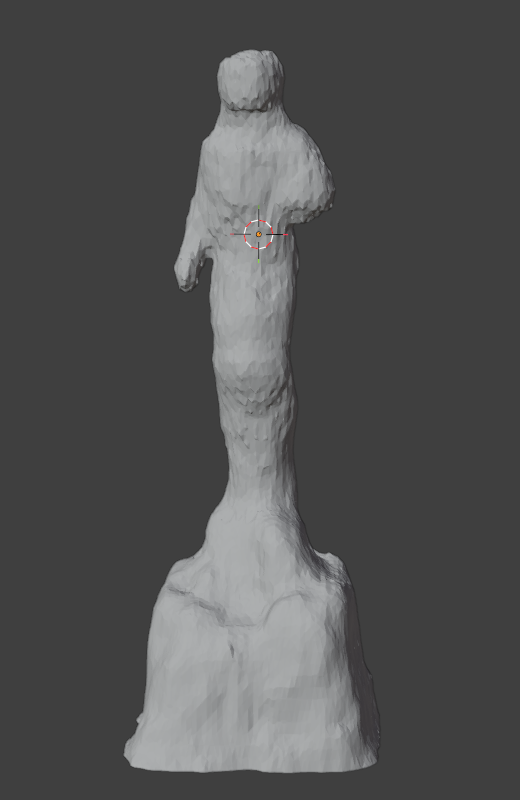
\includegraphics[width=\linewidth]{figures/task1/objectB/astronaut_mesh.png}
		\caption{Astronaut Mesh}
	\end{subfigure}
	\hfill
	\begin{subfigure}{0.25\textwidth}
		\centering
		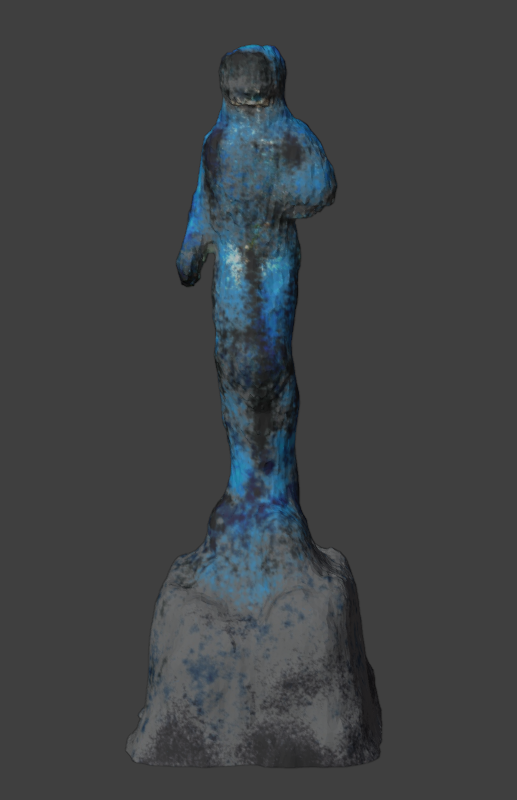
\includegraphics[width=\linewidth]{figures/task1/objectB/astronaut_color.png}
		\caption{Astronaut Color}
		\label{Astronaut Color}
	\end{subfigure}
	\hfill
	\begin{subfigure}{0.25\textwidth}
		\centering
		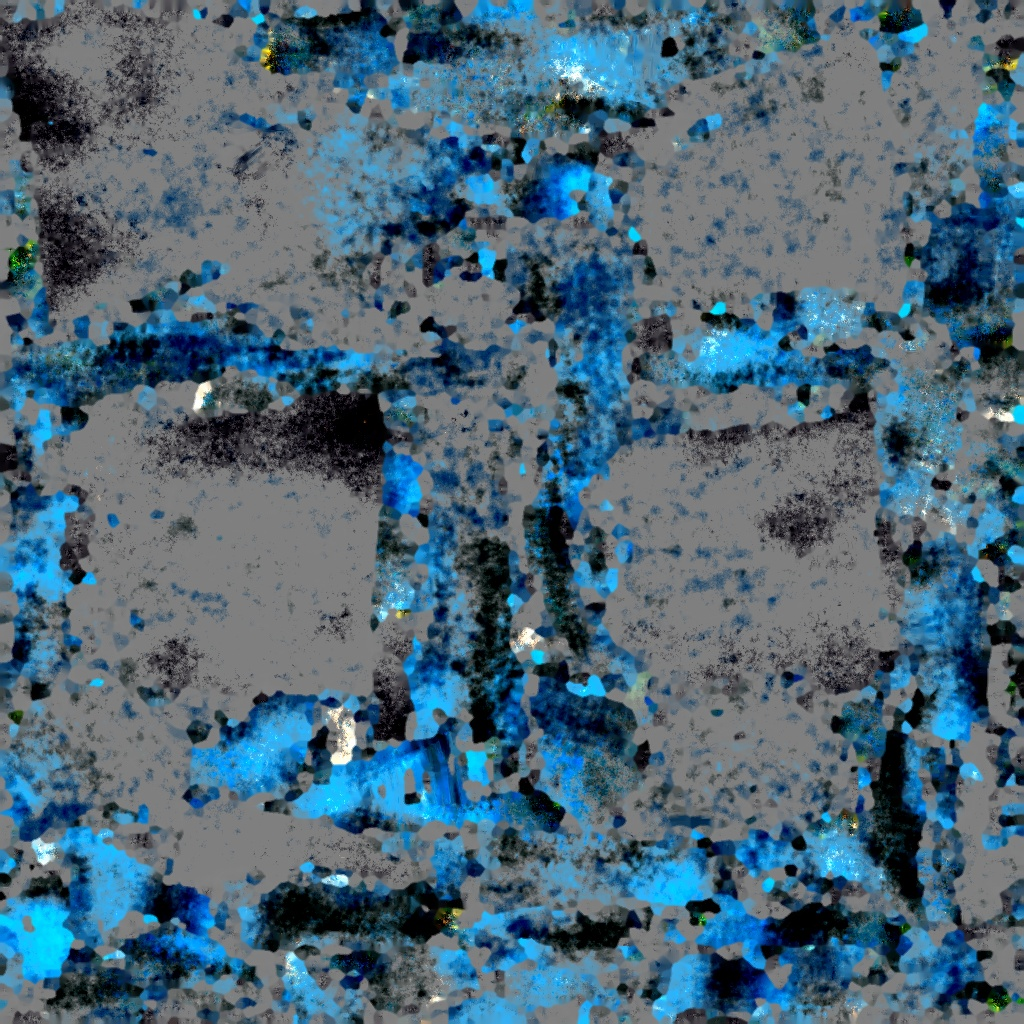
\includegraphics[width=\linewidth]{figures/task1/objectB/astronaut_texture_kd.jpg}
		\caption{Astronaut Texture}
	\end{subfigure}
	
	\vspace{0.6cm}
	
	%================ 第二组：Bunny =================
		% 第一张图（左边）
	\begin{subfigure}{0.8\textwidth}
		\centering
		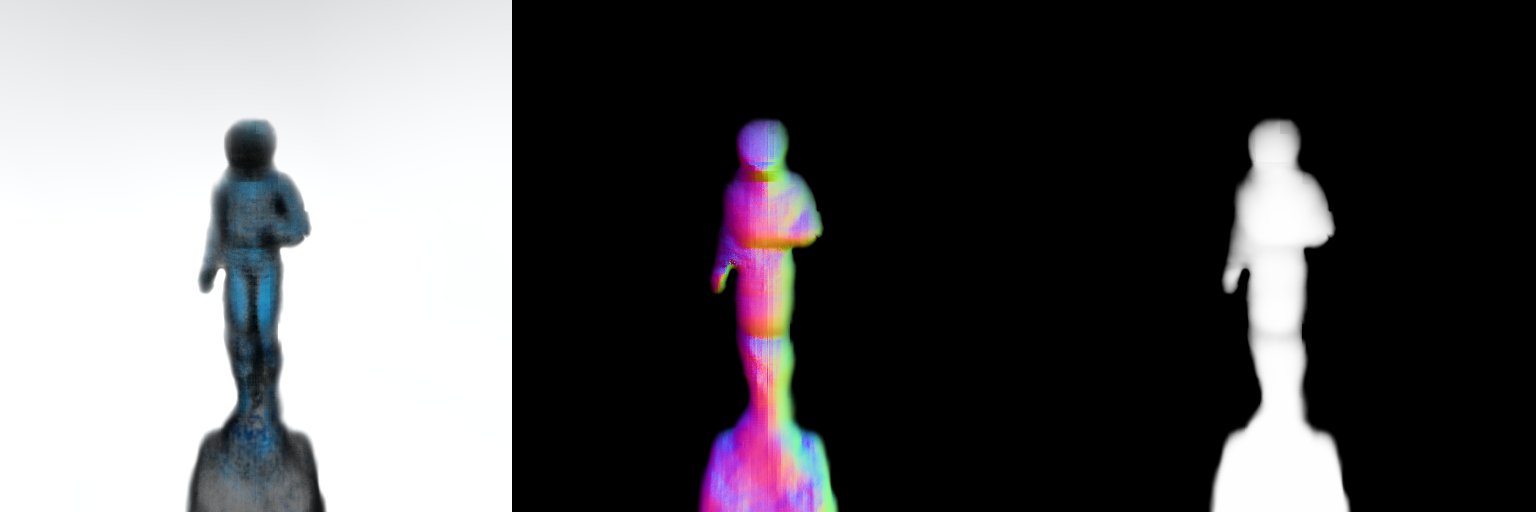
\includegraphics[width=\linewidth]{figures/task1/objectB/astronauts.png} % 替换为你的第一张图片路径
		\caption{Astronauts} % 替换为你想要的图注
	\end{subfigure}
	\hfill % 左右两张图之间的弹性间距

\end{figure}



\begin{figure}[H]
		\begin{subfigure}{0.25\textwidth}
		\centering
		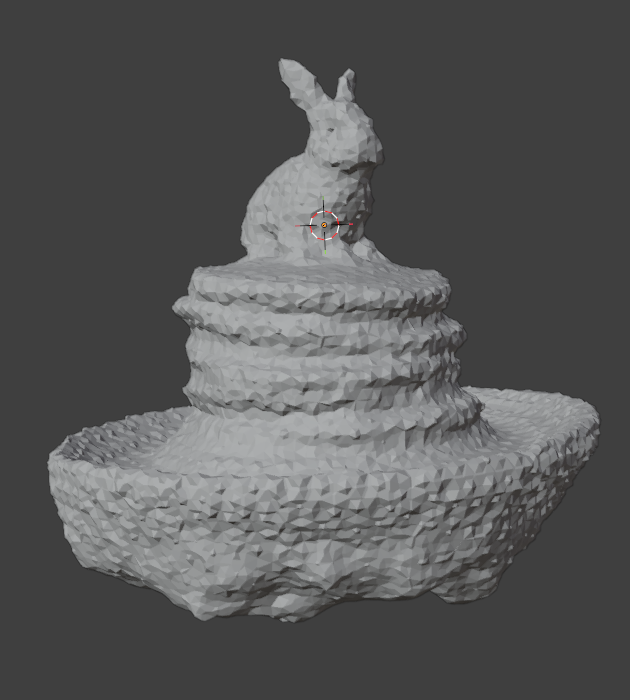
\includegraphics[width=\linewidth]{figures/task1/objectB/bunny_mesh.png}
		\caption{Bunny Mesh}
	\end{subfigure}
	\hfill
	\begin{subfigure}{0.25\textwidth}
		\centering
		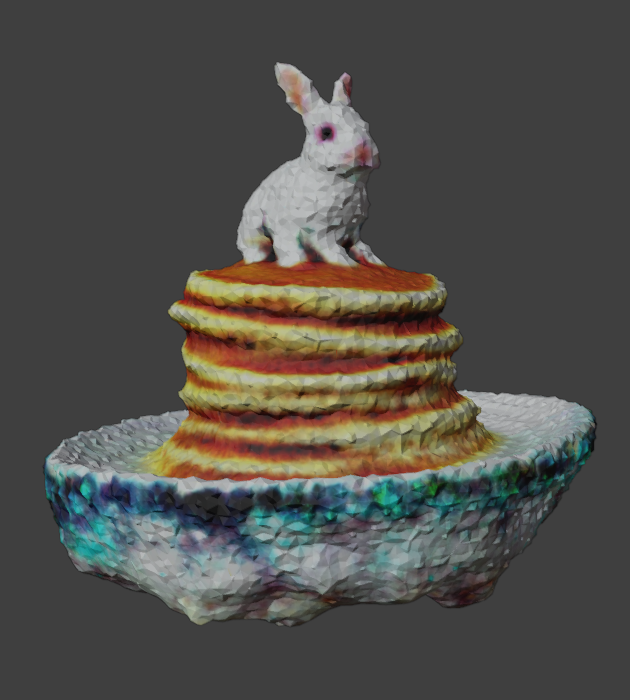
\includegraphics[width=\linewidth]{figures/task1/objectB/bunny_color.png}
		\caption{Bunny Color}
	\end{subfigure}
	\hfill
	\begin{subfigure}{0.25\textwidth}
		\centering
		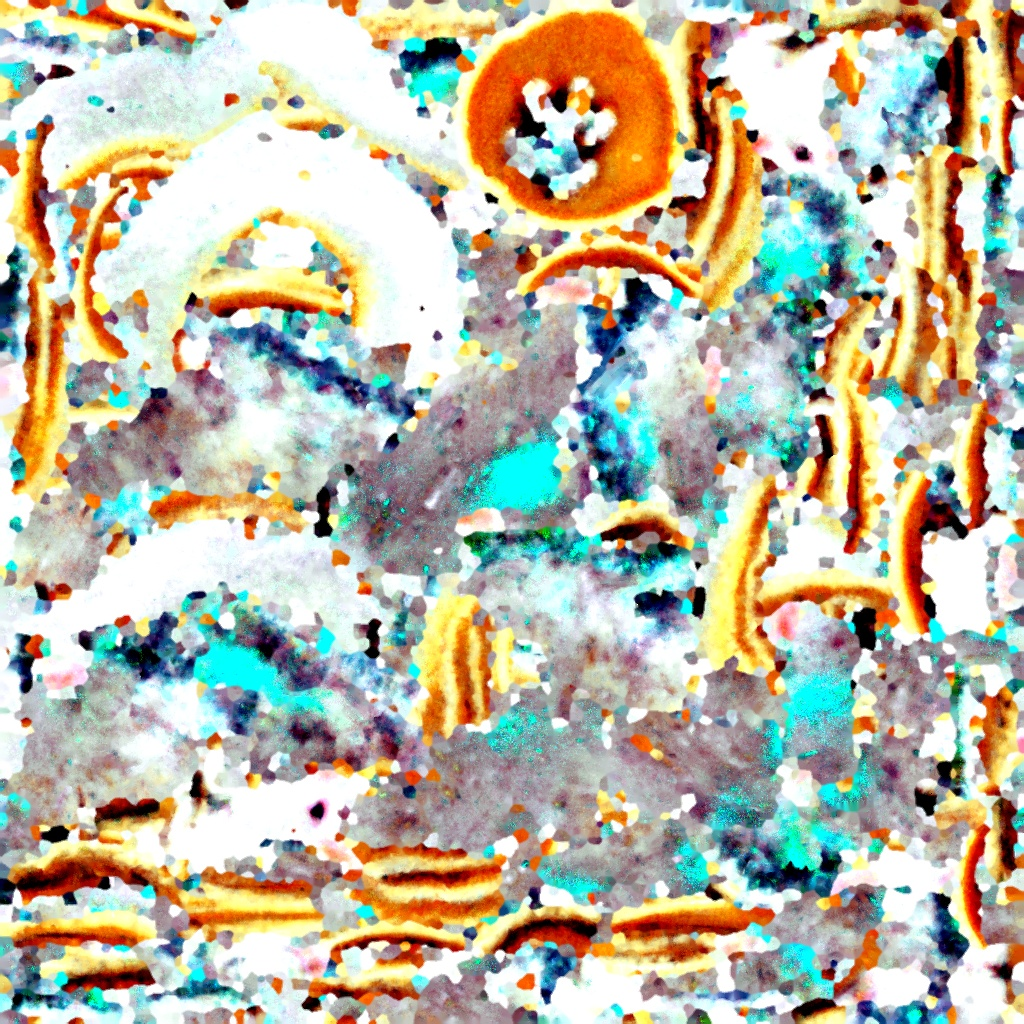
\includegraphics[width=\linewidth]{figures/task1/objectB/bunny_texture_kd.jpg}
		\caption{Bunny Texture}
	\end{subfigure}
	
	\centering
	\vspace{0.6cm}

	% 第二张图（右边）
	\begin{subfigure}{0.8\textwidth}
		\centering
		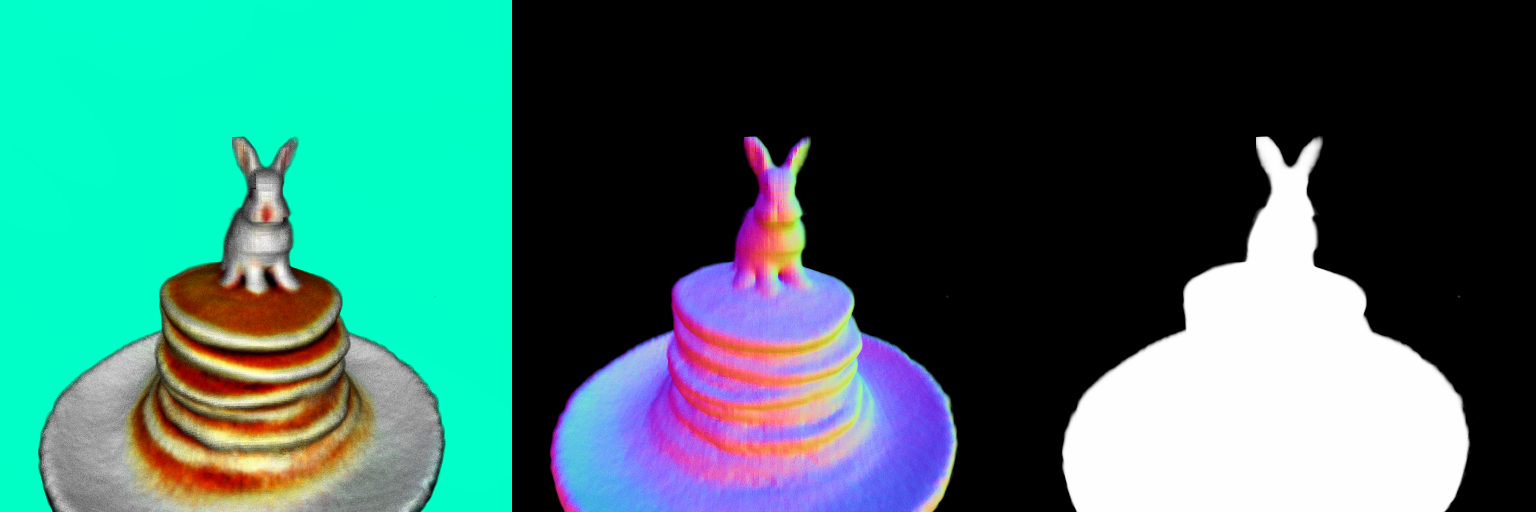
\includegraphics[width=\linewidth]{figures/task1/objectB/bunnys.png} % 替换为你的第二张图片路径
		\caption{Bunnys} % 替换为你想要的图注
	\end{subfigure}

\end{figure}


%================ Loss Functions =================
\begin{figure}[H]
	\centering
	
	% 第一行
	\begin{subfigure}{0.4\textwidth}
		\centering
		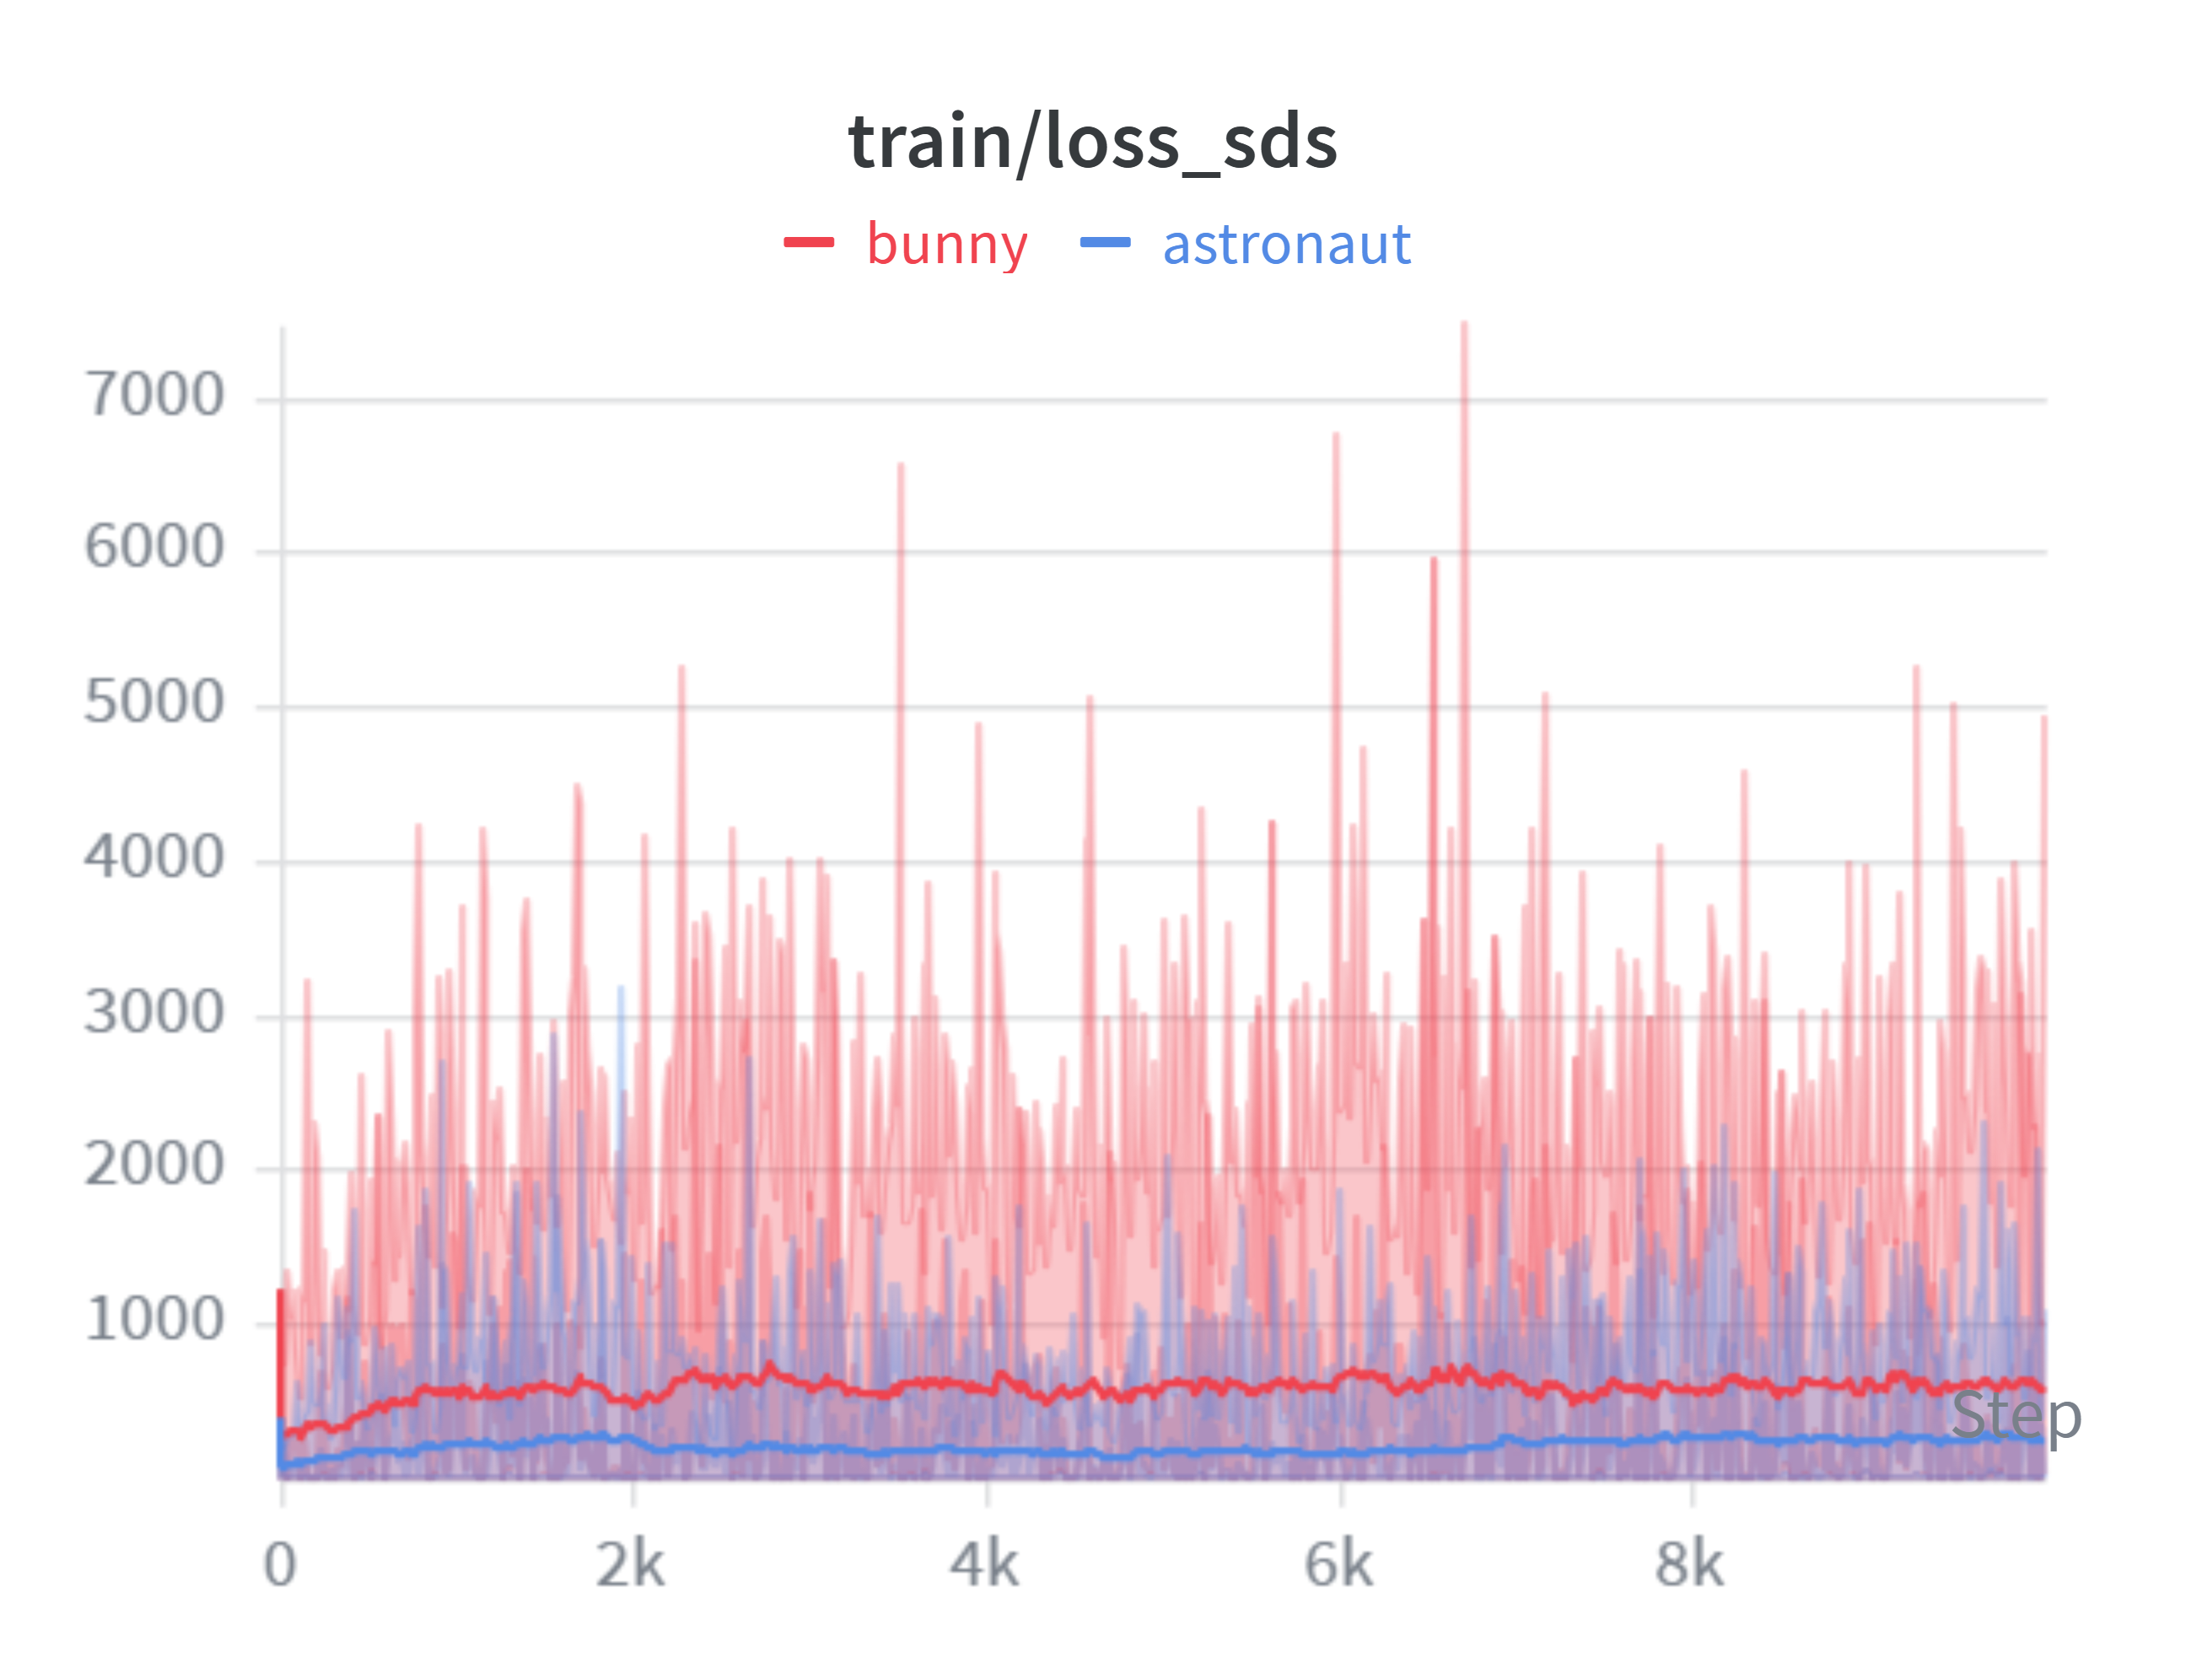
\includegraphics[width=\linewidth]{figures/task1/objectB/sds_loss.png}
		\caption{SDS Loss}
	\end{subfigure}
	\hfill
	\begin{subfigure}{0.4\textwidth}
		\centering
		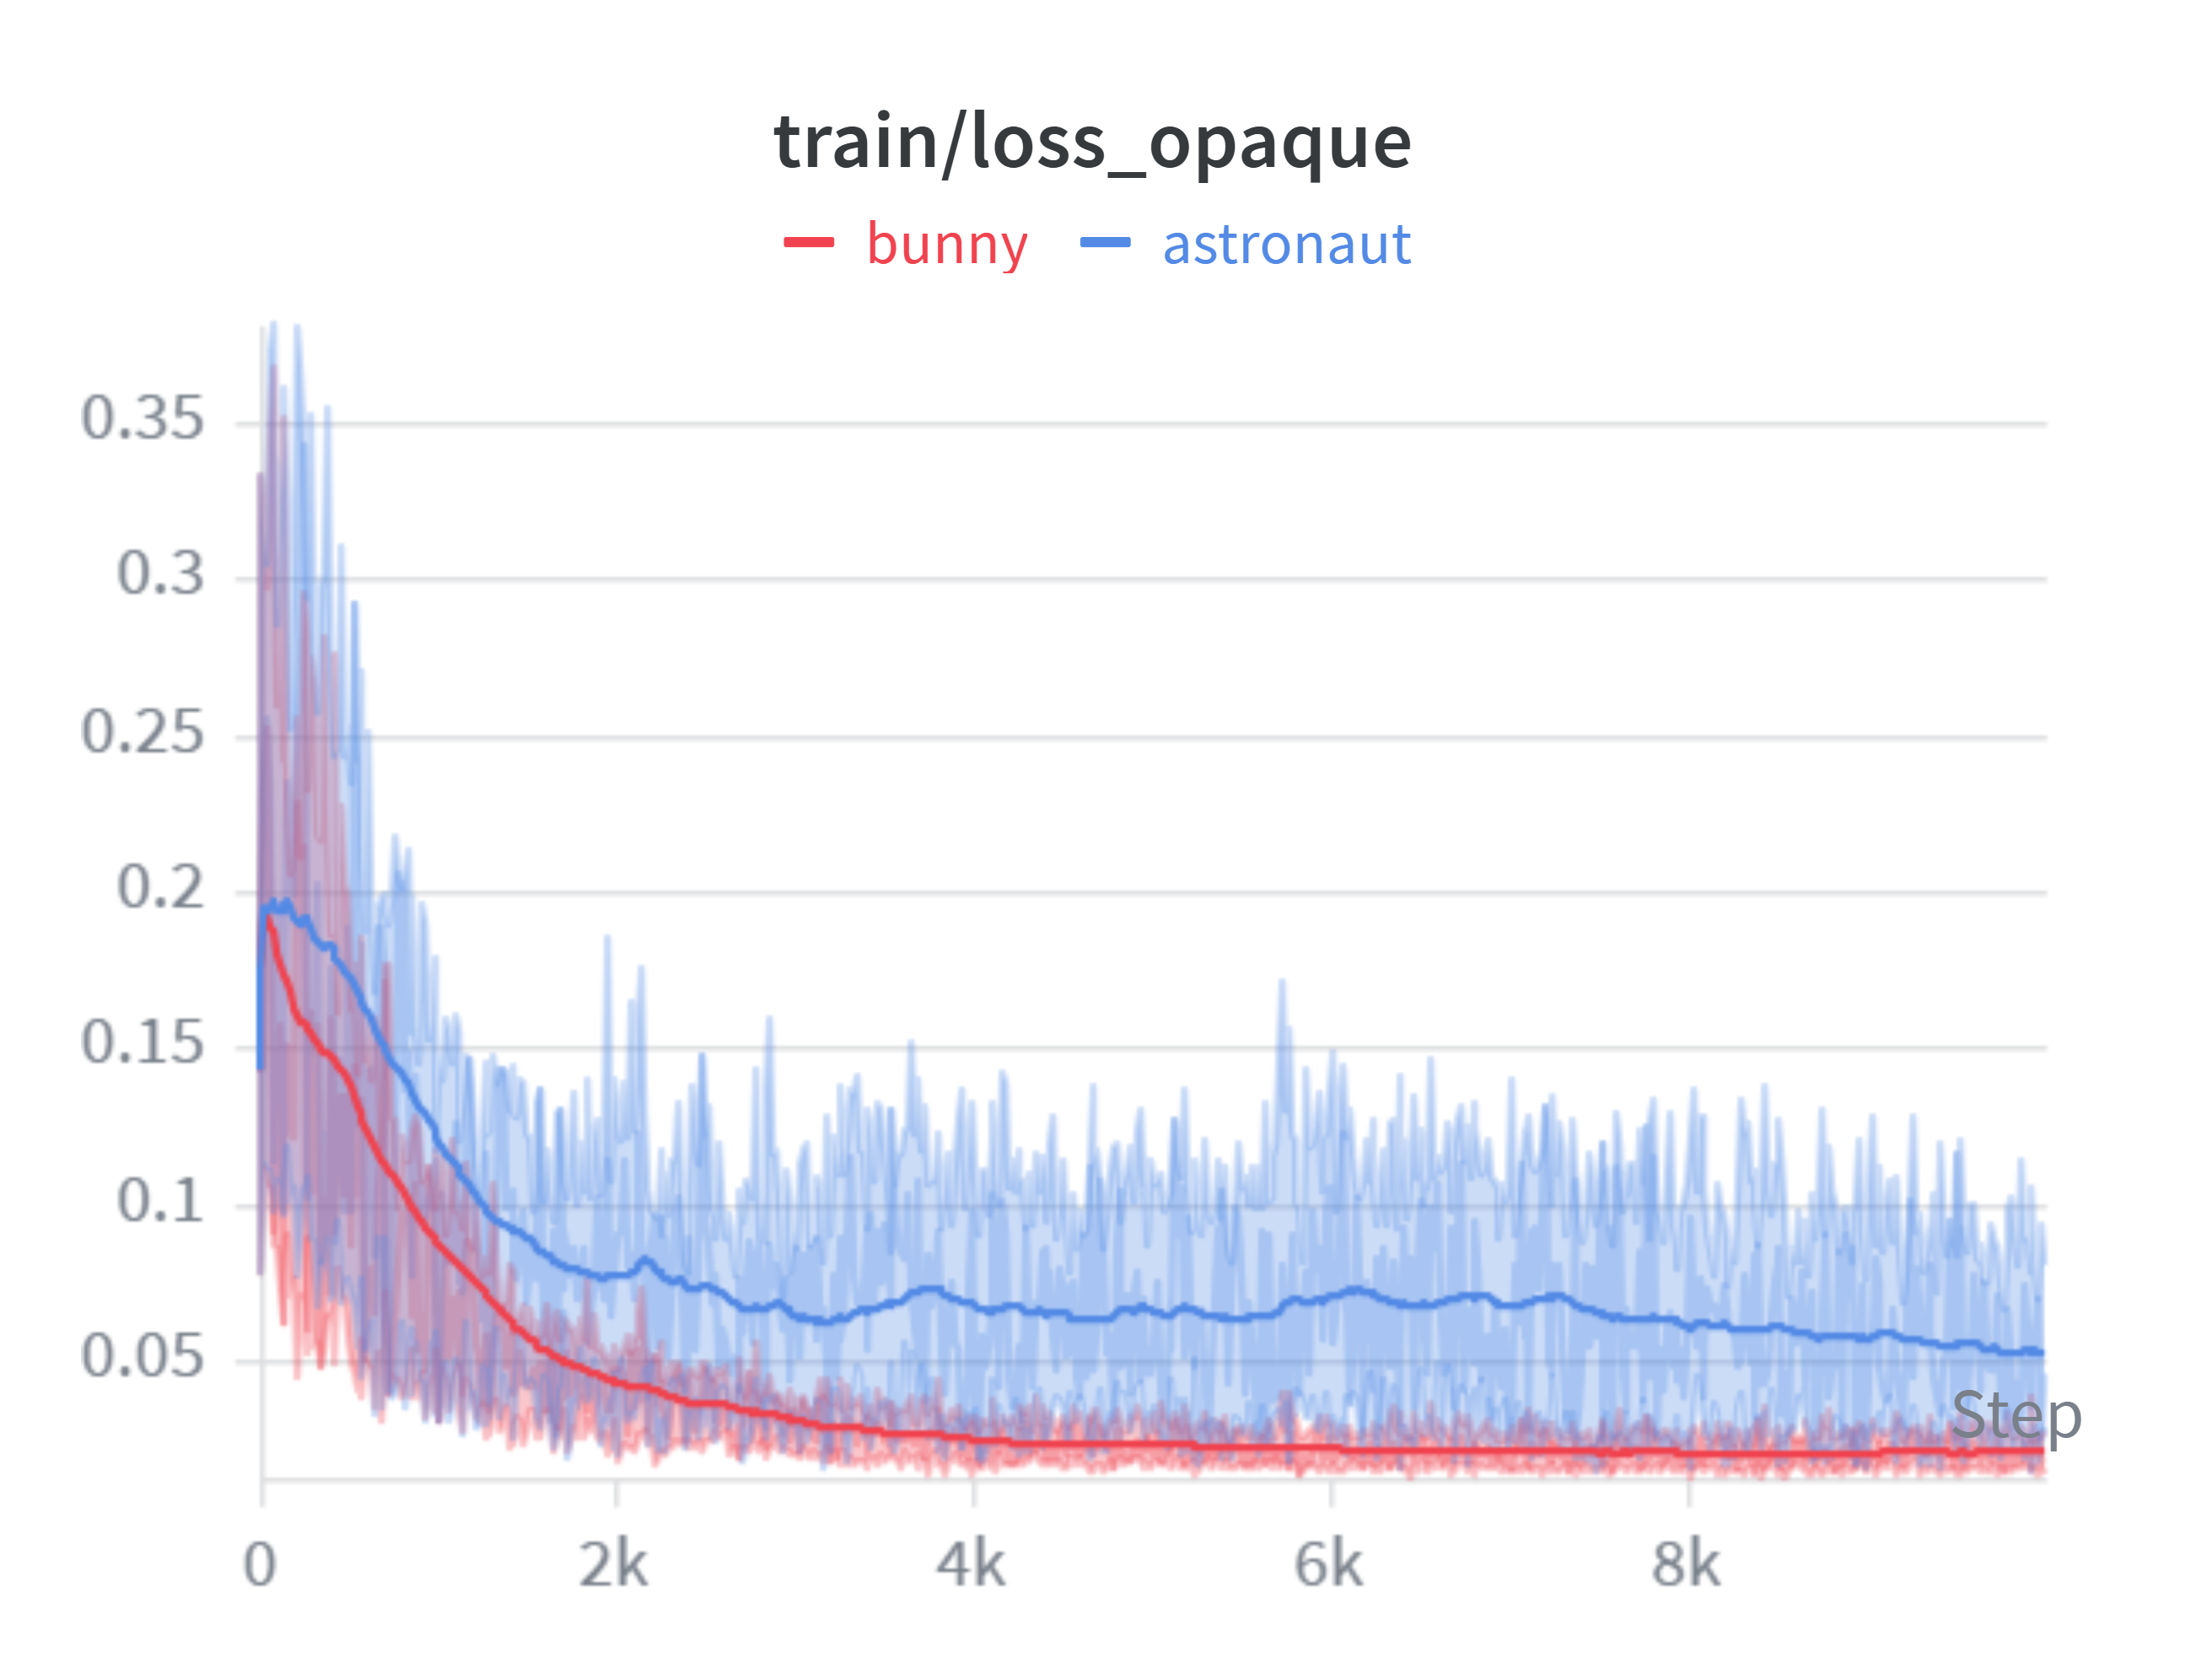
\includegraphics[width=\linewidth]{figures/task1/objectB/opaque_loss.png}
		\caption{Opaque Loss}
	\end{subfigure}
	
	\vspace{0.5cm} % 行间距，可以根据需要调整
	
	% 第二行
	\begin{subfigure}{0.4\textwidth}
		\centering
		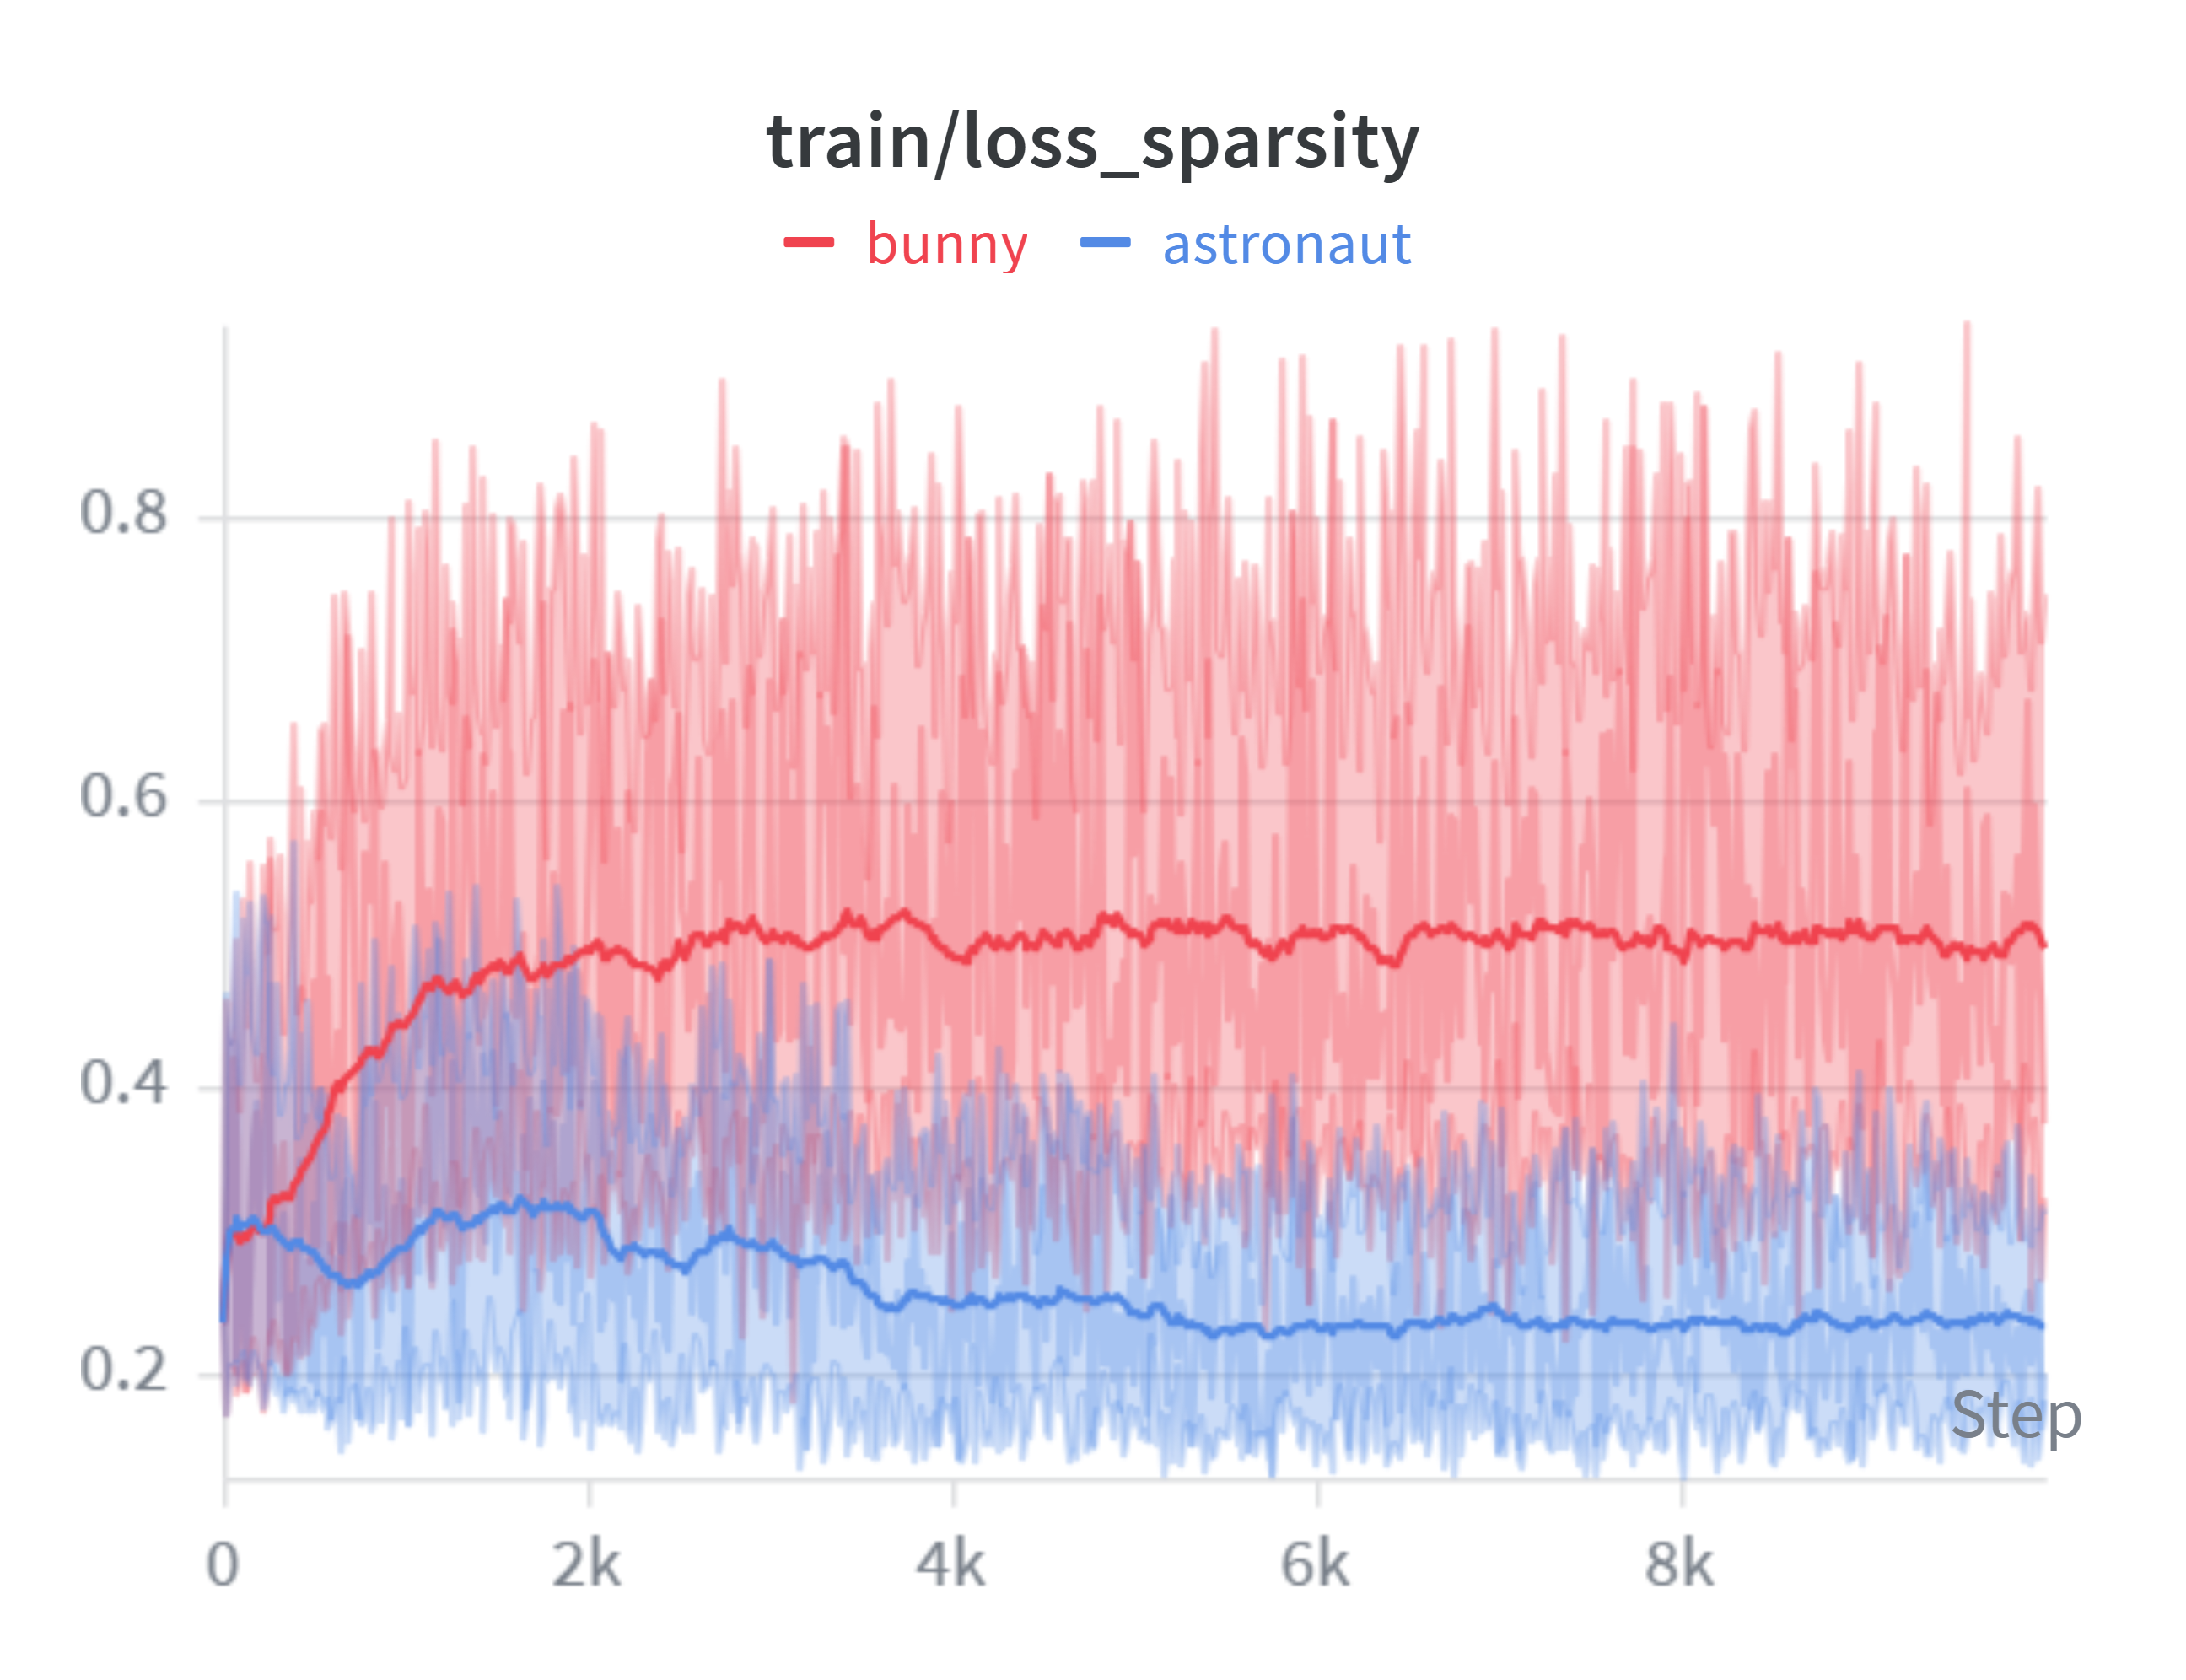
\includegraphics[width=\linewidth]{figures/task1/objectB/sparsity_loss.png}
		\caption{Sparsity Loss}
	\end{subfigure}
	\hfill
	\begin{subfigure}{0.4\textwidth}
		\centering
		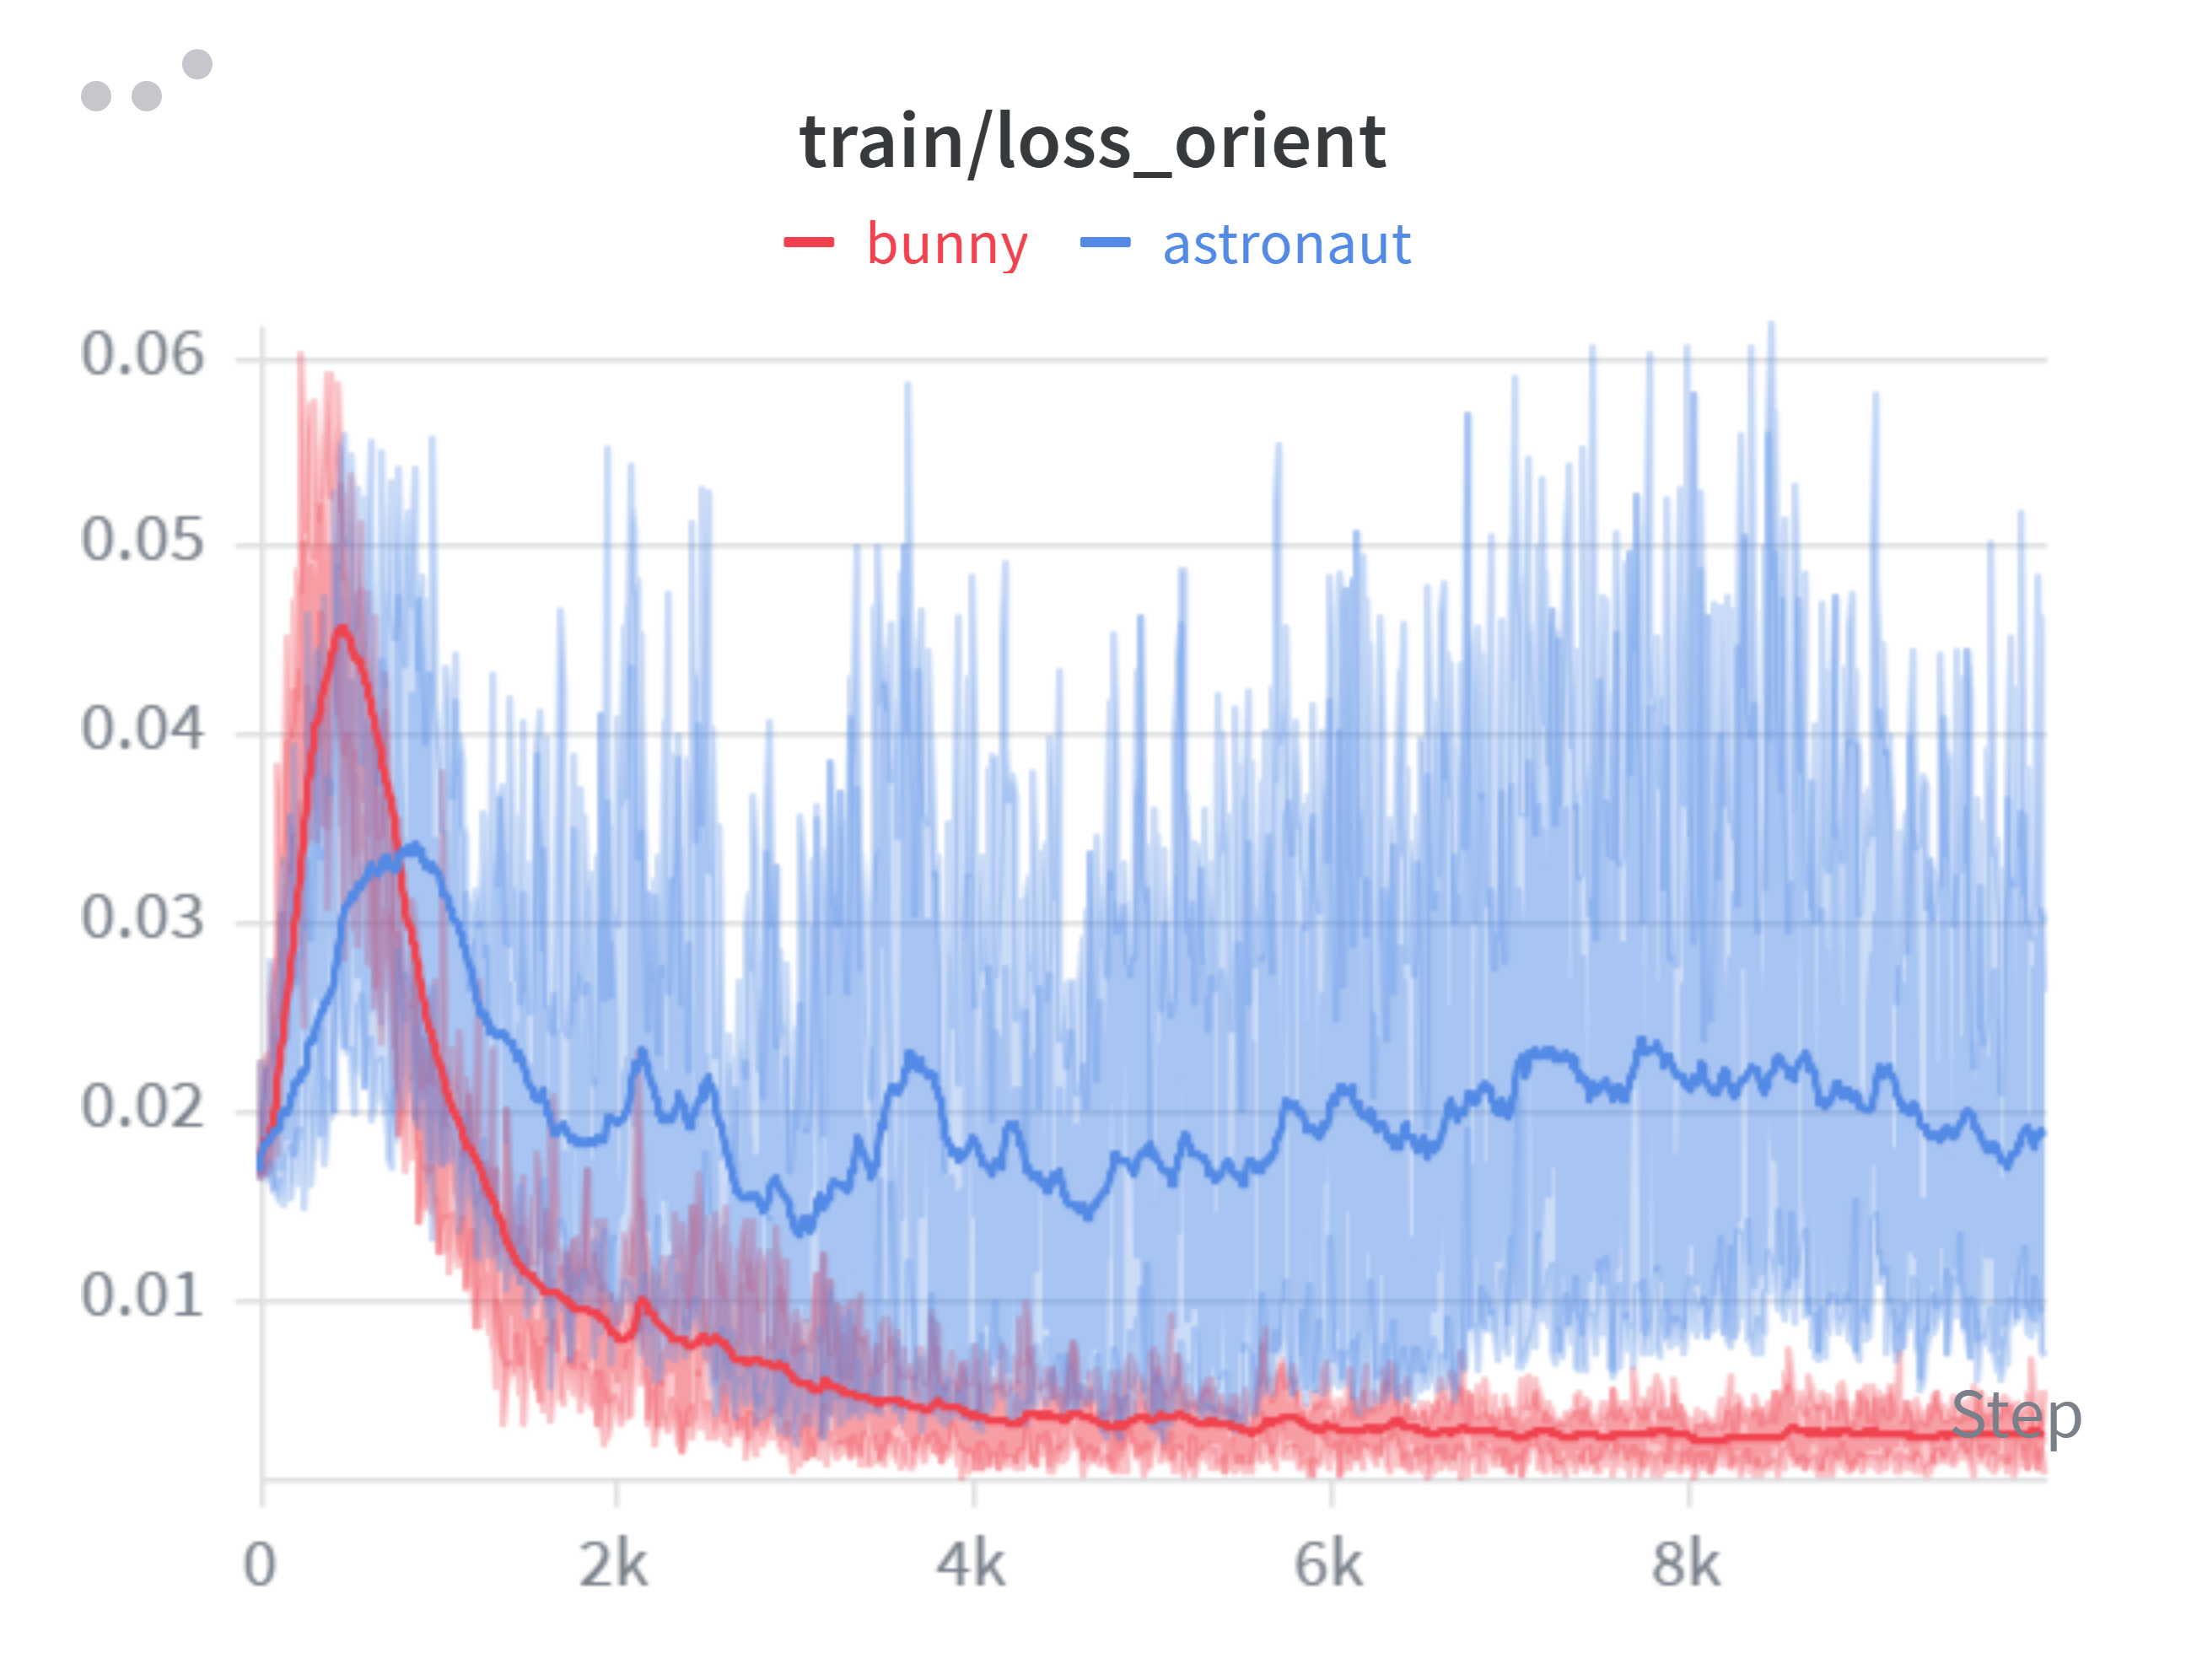
\includegraphics[width=\linewidth]{figures/task1/objectB/orient_loss.png}
		\caption{Orient Loss}
	\end{subfigure}
	
	\caption{Visualization results of generated 3D objects and training loss functions.}
	\label{fig:results_and_losses}
\end{figure}

We can see from the model visualizations that the astronaut has a relatively less smoother outfit and less appropriate color distribution, this may because that the pre-trained model doesn't have enough information compared with the bunny.

As for the training dynamics, here are our analysis:

SDS Loss exhibits extremely large magnitude values, reaching into the thousands, accompanied by very high variance and strong oscillations. Unlike typical supervised learning objectives, it does not demonstrate a smooth and monotonic decreasing trend during optimization. In 3D generative tasks, SDS Loss is derived from a pretrained diffusion model and fundamentally provides gradient directions in the parameter space rather than serving as an absolute scalar objective to be minimized to zero. Therefore, this behavior is ordinary. Comparing the two objects, the Bunny (red curve) shows significantly higher baseline values and variance than the Astronaut (blue curve), suggesting that the diffusion model provides more uncertain or higher-variance gradient guidance for the Bunny, possibly due to a more complex and unsmooth structure of the astronaut.

Opaque Loss decreases rapidly during the early stages of training and then gradually approaches a stable asymptotic plateau. This loss typically acts as a regularization term that removes floating artifacts and encourages the model to produce solid geometry. The Bunny converges very quickly and stabilizes near zero with minimal noise, whereas the Astronaut also decreases but eventually stabilizes at a relatively higher mean value (approximately 0.05 to 0.1) and retains noticeable variance in later stages. This indicates that the Astronaut presents a more challenging optimization landscape for opacity regularization.But the total structure is still clear.

Sparsity Loss increases rapidly in the early training stage before entering a highly oscillatory plateau. This reflects the constraint on spatial occupancy, encouraging empty space outside the object region. The initial increase indicates that the model is expanding its occupied volume while constructing the coarse geometry, while the subsequent plateau reflects a dynamic equilibrium between forming complete structures and maintaining spatial sparsity. The Bunny stabilizes at a relatively higher level (around 0.5), while the Astronaut stabilizes at a lower value (around 0.2). Suggesting that the Bunny occupies a more spatially extensive or volumetrically dense structure, resulting in higher sparsity penalties,which is aligned with the visualization results.

Orient Loss demonstrates a characteristic “spike-then-decay” behavior. This loss is typically used to regularize surface normals, ensuring smooth and physically consistent surface orientations while preventing jagged artifacts. The initial spike occurs when the model begins forming its coarse geometry and surface normals are highly disordered. As training progresses and the geometry becomes smoother, the loss decreases and converges. The Bunny reaches its peak around 1000 steps and then converges smoothly toward near-zero values, indicating highly optimized surface smoothness. In contrast, the Astronaut peaks slightly earlier but retains higher fluctuations and a non-negligible residual value (around 0.02), suggesting that its surface geometry is more complex.








\subsubsection{Object C}
In this section, the following picture is trained:

\begin{figure}[H]
	\centering
	
	% 第一张图（左边）
	\begin{subfigure}{0.4\textwidth}
		\centering
		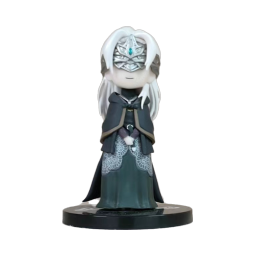
\includegraphics[width=\linewidth]{figures/task1/objectC/firekeeper_rgba.png} % 第一张图片路径
		\caption{Firekeeper(threestudio)}
	\end{subfigure}
	\hfill % 两张图之间的间距
	% 第二张图（右边）
	\begin{subfigure}{0.4\textwidth}
		\centering
		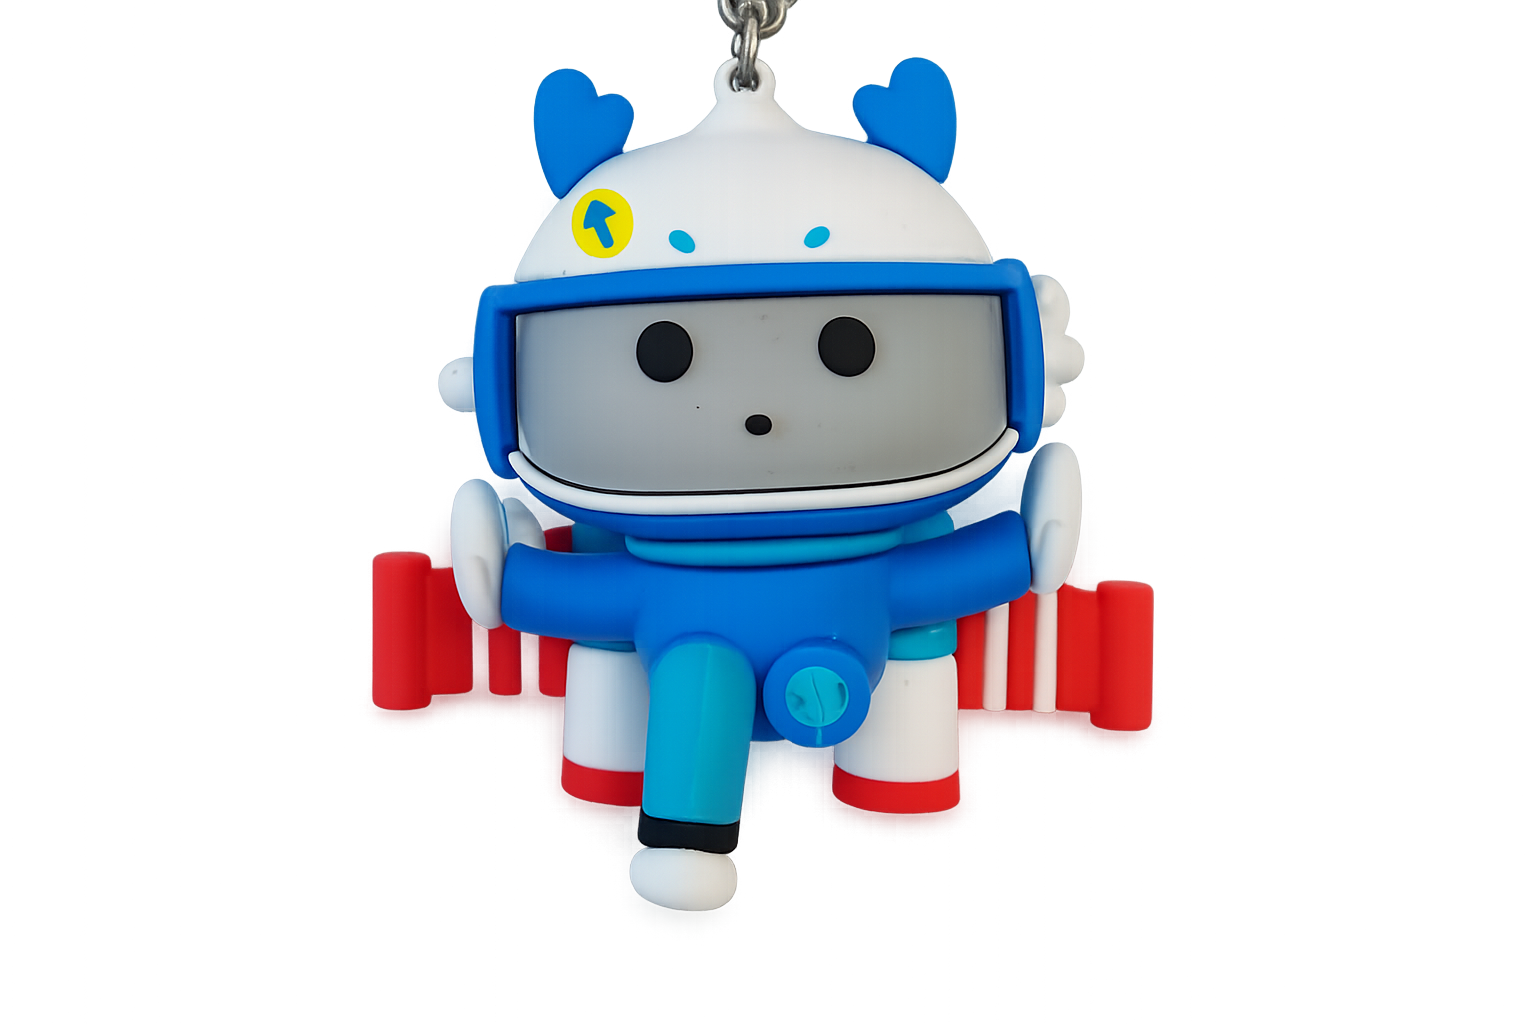
\includegraphics[width=\linewidth]{figures/task1/objectC/cute_robot_rgba.png} % 替换为你的第二张图片路径
		\caption{Cute Astronaut Robot(Ours)}
	\end{subfigure}

\end{figure}


Each training takes about \textbf{30min}(coarse)+\textbf{30min}(refine), the rendering results and training dynamics are as follow:

\begin{figure}[H]
	\centering
	
	%================ 第一组：Astronaut =================
	\begin{subfigure}{0.25\textwidth}
		\centering
		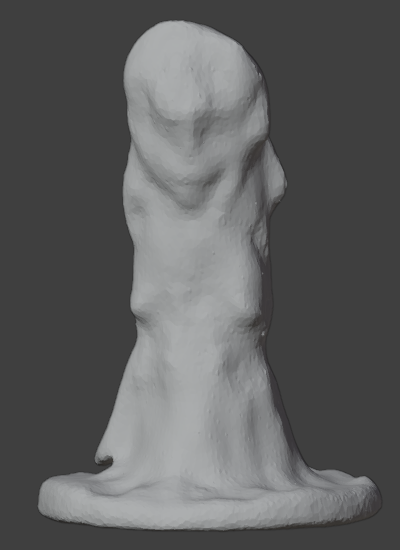
\includegraphics[width=\linewidth]{figures/task1/objectC/firekeeper_mesh.png}
		\caption{Firekeeper Mesh}
	\end{subfigure}
	\hfill
	\begin{subfigure}{0.25\textwidth}
		\centering
		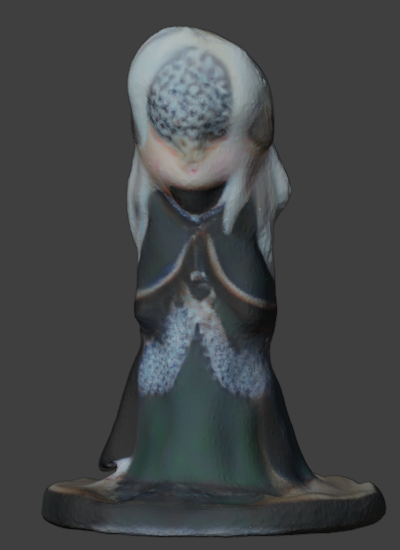
\includegraphics[width=\linewidth]{figures/task1/objectC/firekeeper_color.png}
		\caption{Firekeeper Color}
	\end{subfigure}
	\hfill
	\begin{subfigure}{0.25\textwidth}
		\centering
		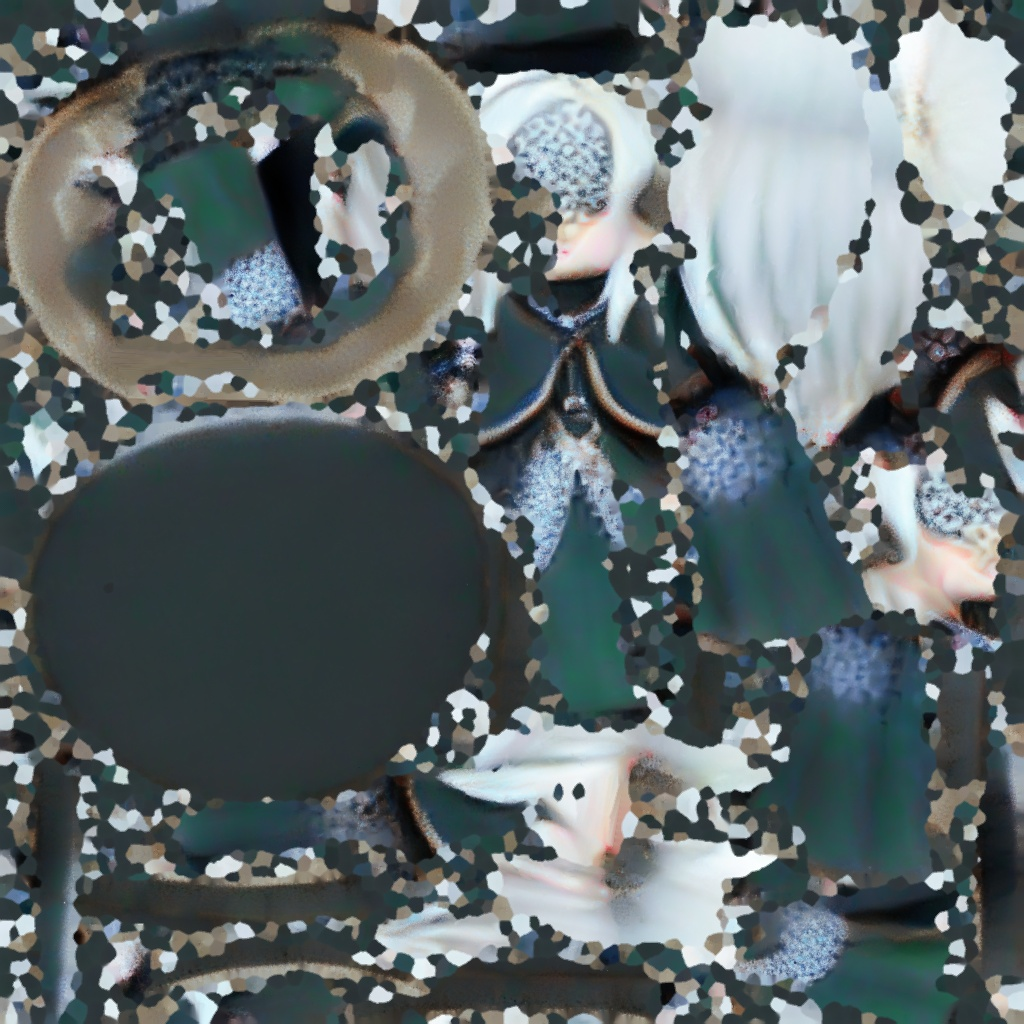
\includegraphics[width=\linewidth]{figures/task1/objectC/firekeeper_texture_kd.jpg}
		\caption{Firekeeper Texture}
	\end{subfigure}
	
	
\end{figure}




\begin{figure}[H]
	\centering
	
	% 第一张
	
\includegraphics[width=0.6\textwidth]{figures/task1/objectC/firekeeper1.png} % 替换为你的实际路径

	
	\vspace{0.3cm} % 调整图片之间的垂直间距
	
	% 第二张
	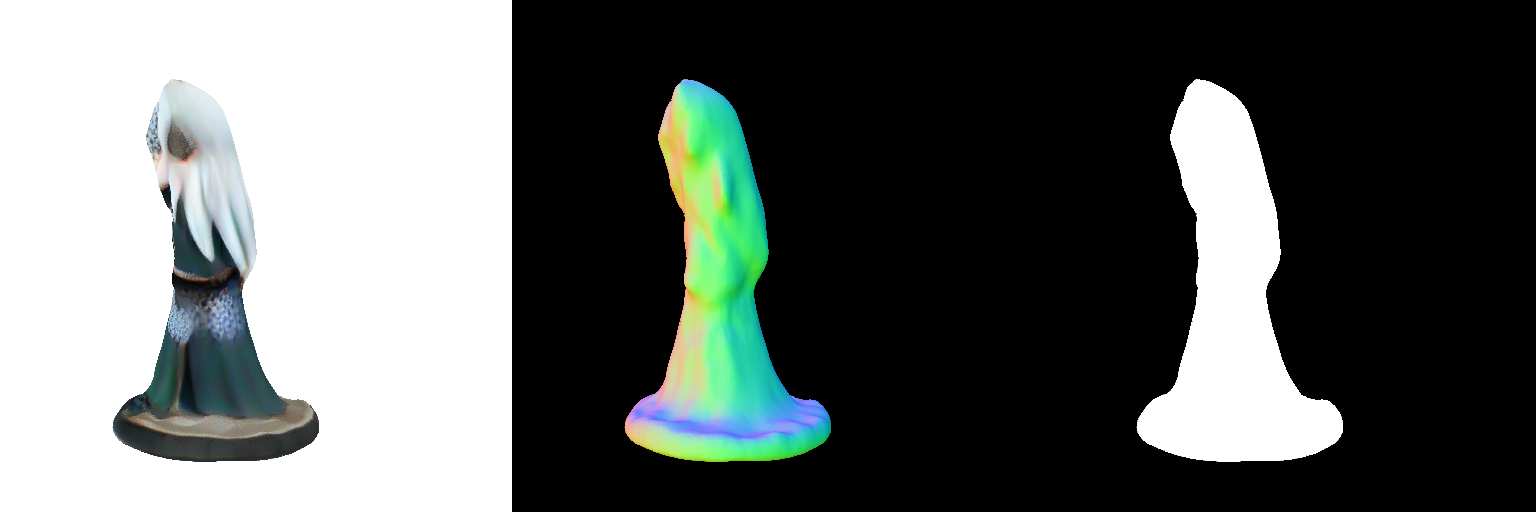
\includegraphics[width=0.6\textwidth]{figures/task1/objectC/firekeeper2.png}

	
	\vspace{0.3cm}
	
	% 第三张
	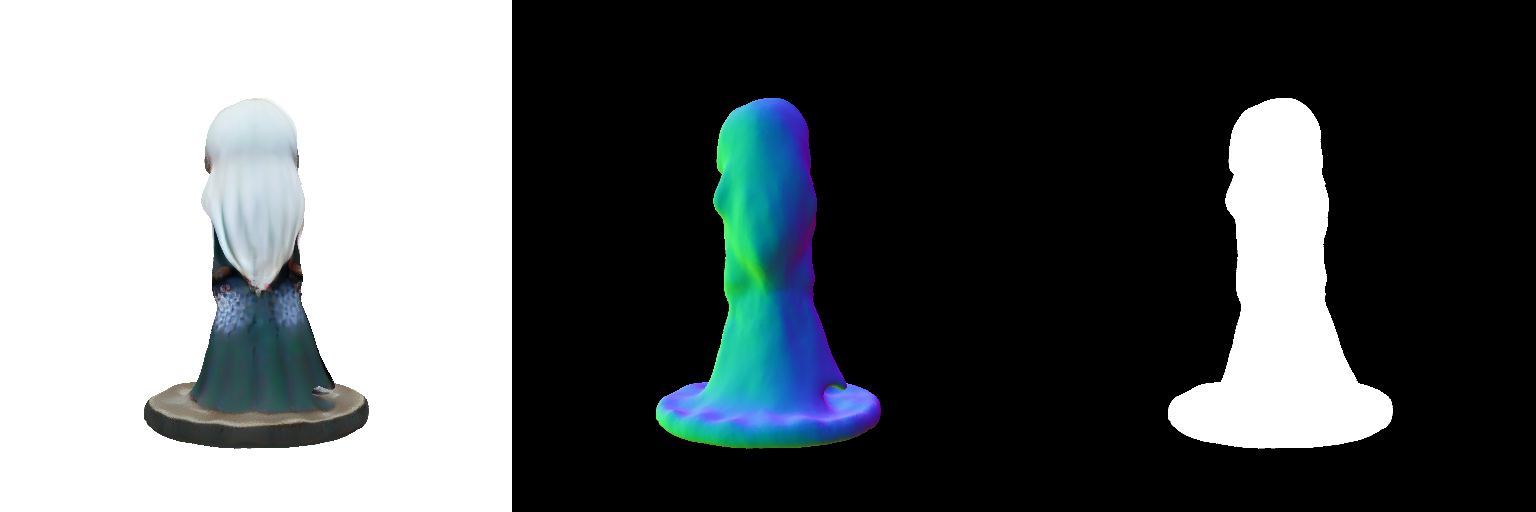
\includegraphics[width=0.6\textwidth]{figures/task1/objectC/firekeeper3.png}

	
	\vspace{0.3cm}
	
	% 第四张
	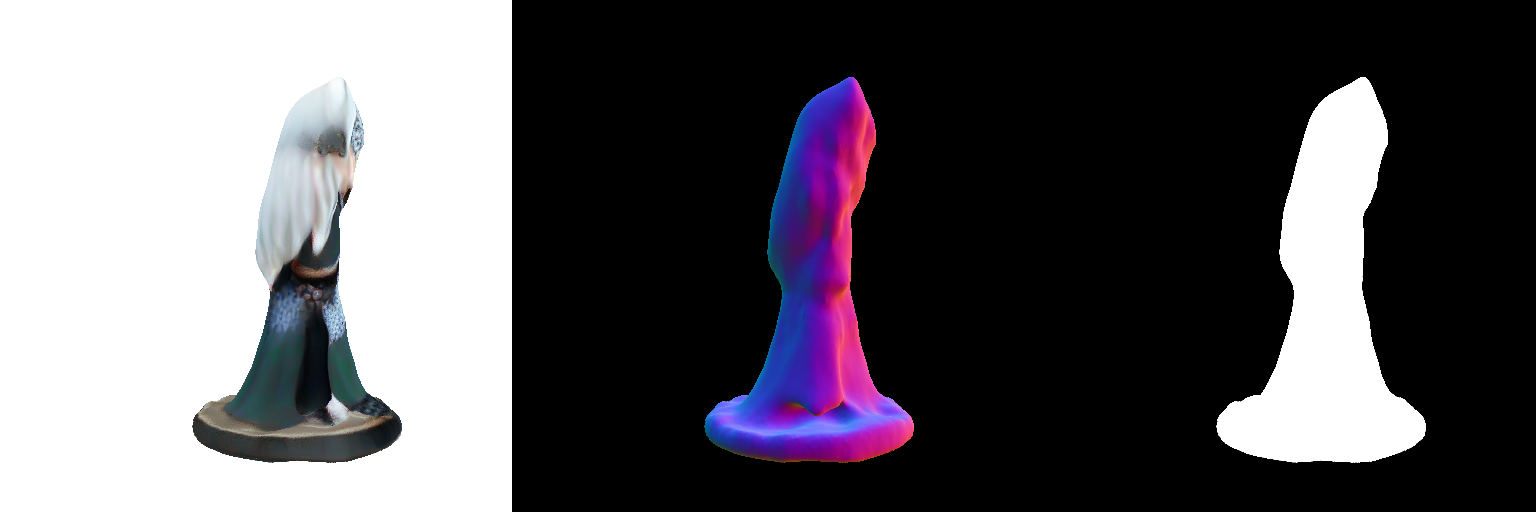
\includegraphics[width=0.6\textwidth]{figures/task1/objectC/firekeeper4.png}

	
	\caption{Different Viewpoints}
	\label{fig:firekeeper_vertical}
\end{figure}

\begin{figure}[H]
		\begin{subfigure}{0.25\textwidth}
		\centering
		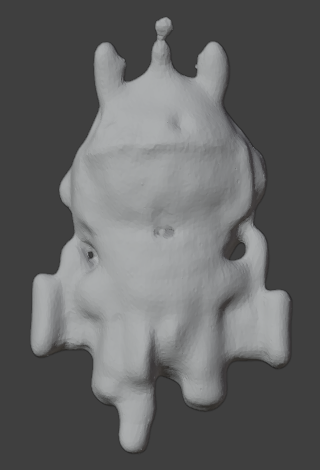
\includegraphics[width=\linewidth]{figures/task1/objectC/cute_robot_mesh.png}
		\caption{Robot Mesh}
	\end{subfigure}
	\hfill
	\begin{subfigure}{0.25\textwidth}
		\centering
		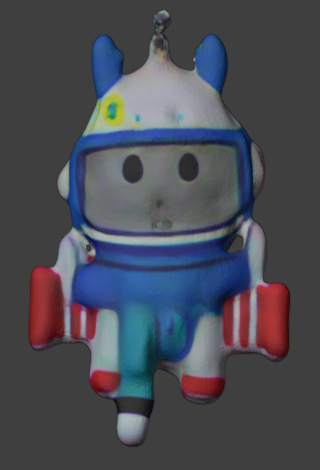
\includegraphics[width=\linewidth]{figures/task1/objectC/cute_robot_color.png}
		\caption{Robot Color}
	\end{subfigure}
	\hfill
	\begin{subfigure}{0.25\textwidth}
		\centering
		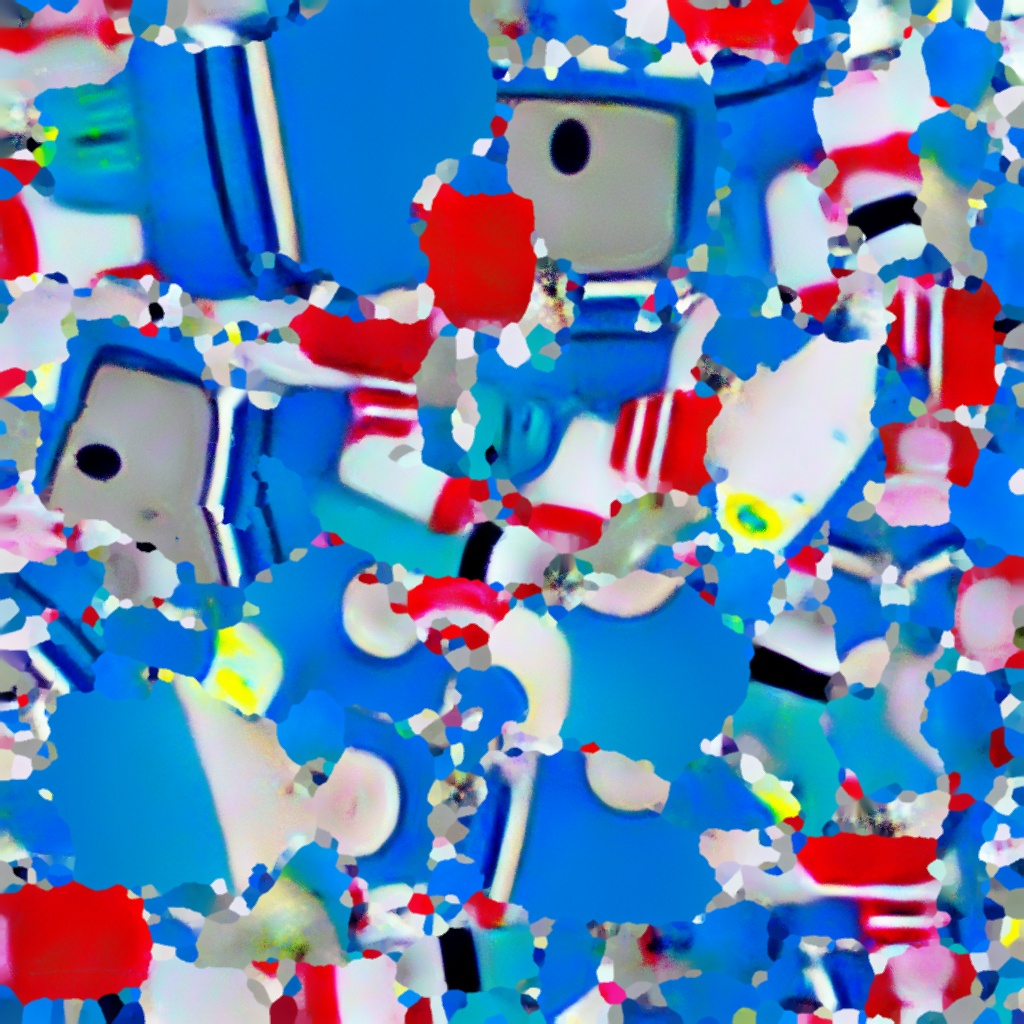
\includegraphics[width=\linewidth]{figures/task1/objectC/robot_texture_kd.jpg}
		\caption{Robot Texture}
	\end{subfigure}
\end{figure}

\begin{figure}[H]
	\centering
	
	% 第一张
	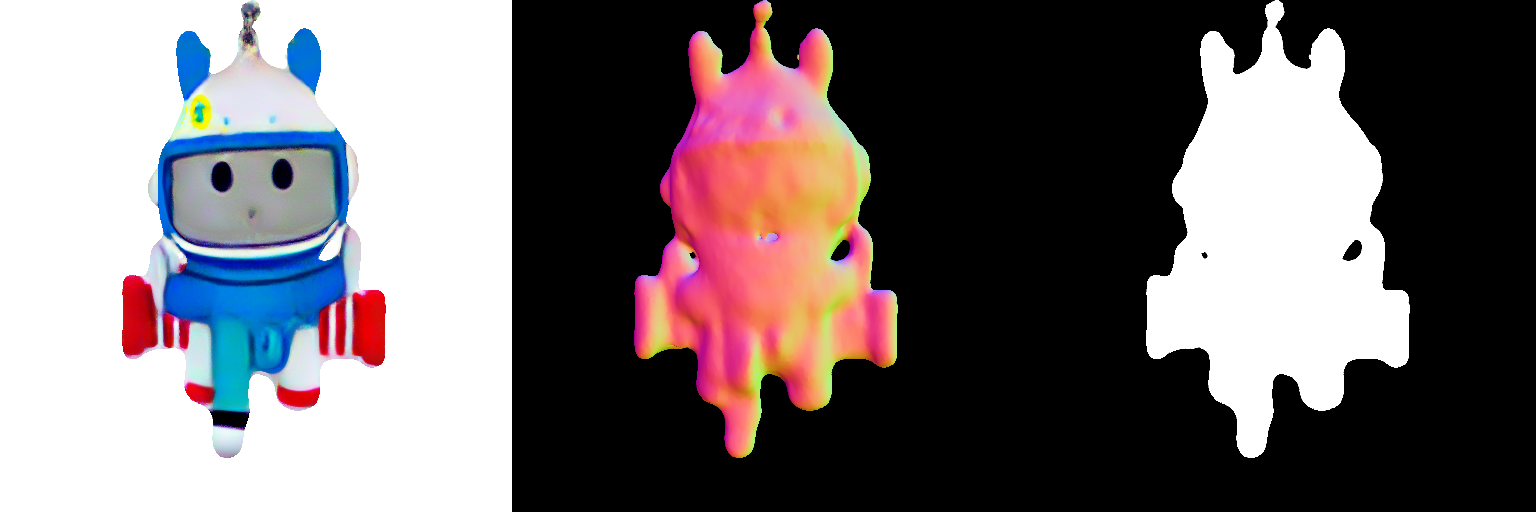
\includegraphics[width=0.6\textwidth]{figures/task1/objectC/robot1.png} % 替换为你的实际路径
	
	
	\vspace{0.3cm} % 调整图片之间的垂直间距
	
	% 第二张
	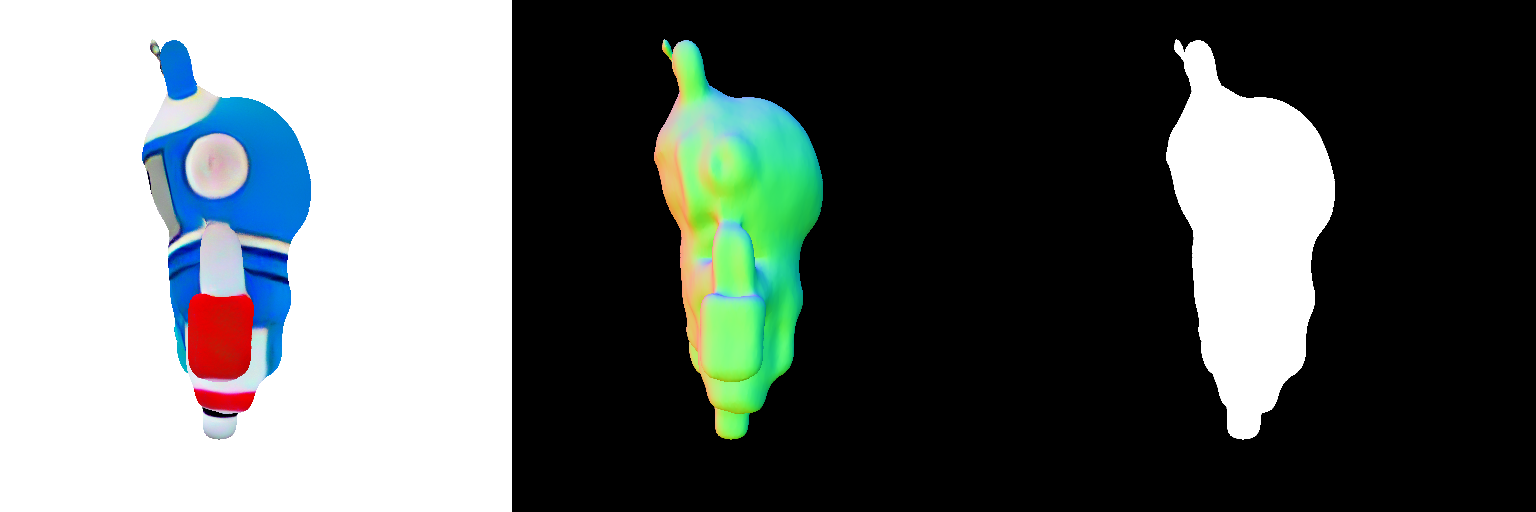
\includegraphics[width=0.6\textwidth]{figures/task1/objectC/robot2.png}
	
	
	\vspace{0.3cm}
	
	% 第三张
	
\includegraphics[width=0.6\textwidth]{figures/task1/objectC/robot3.png}
	
	
	\vspace{0.3cm}
	
	% 第四张
	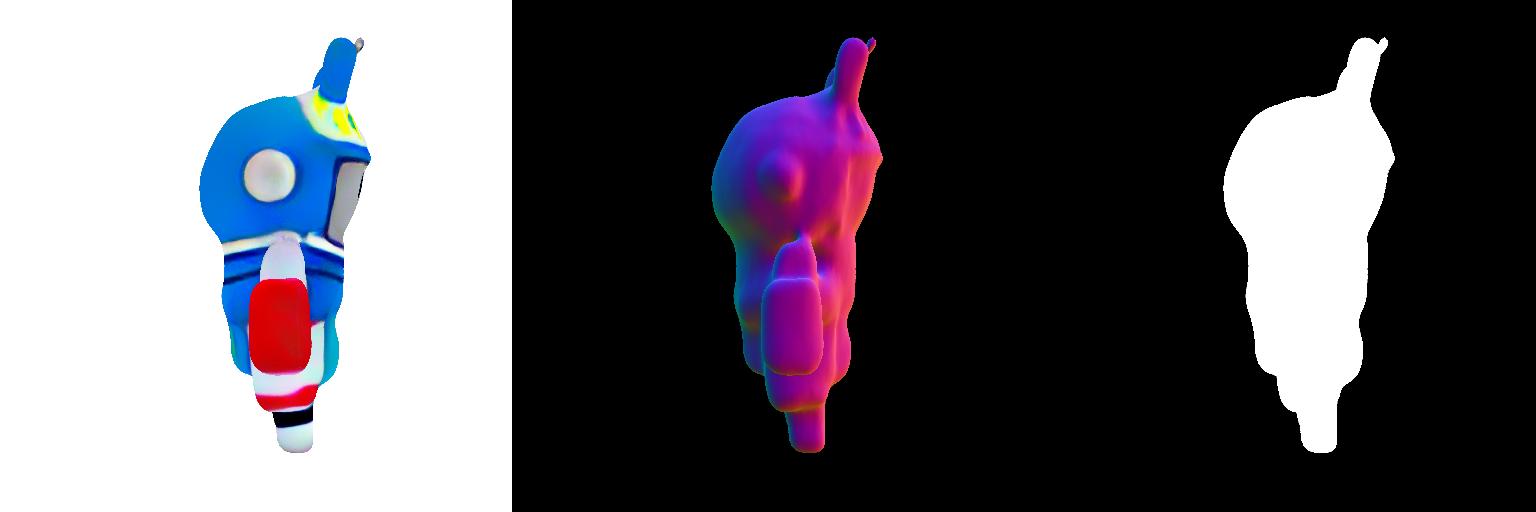
\includegraphics[width=0.6\textwidth]{figures/task1/objectC/robot4.png}
	
	
	\caption{Different Viewpoints}
	\label{fig:Robot_vertical}
\end{figure}



\begin{figure}[H]
	\centering
	
	% 第一张图（左边）
	\begin{subfigure}{0.48\textwidth}
		\centering
		
\includegraphics[width=\linewidth]{figures/task1/objectC/opaque_loss.png} % 第一张图片路径
		\caption{Firekeeper(threestudio)}
	\end{subfigure}
	\hfill % 两张图之间的间距
	% 第二张图（右边）
	\begin{subfigure}{0.48\textwidth}
		\centering
		
\includegraphics[width=\linewidth]{figures/task1/objectC/sparsity_loss.png} % 替换为你的第二张图片路径
		\caption{Cute Astronaut Robot(Ours)}
	\end{subfigure}
	
\end{figure}


\begin{figure*}[H]
	\centering
	
	%==================== 第一组：SDS Loss ====================
	\begin{subfigure}[t]{0.32\textwidth}
		\centering
		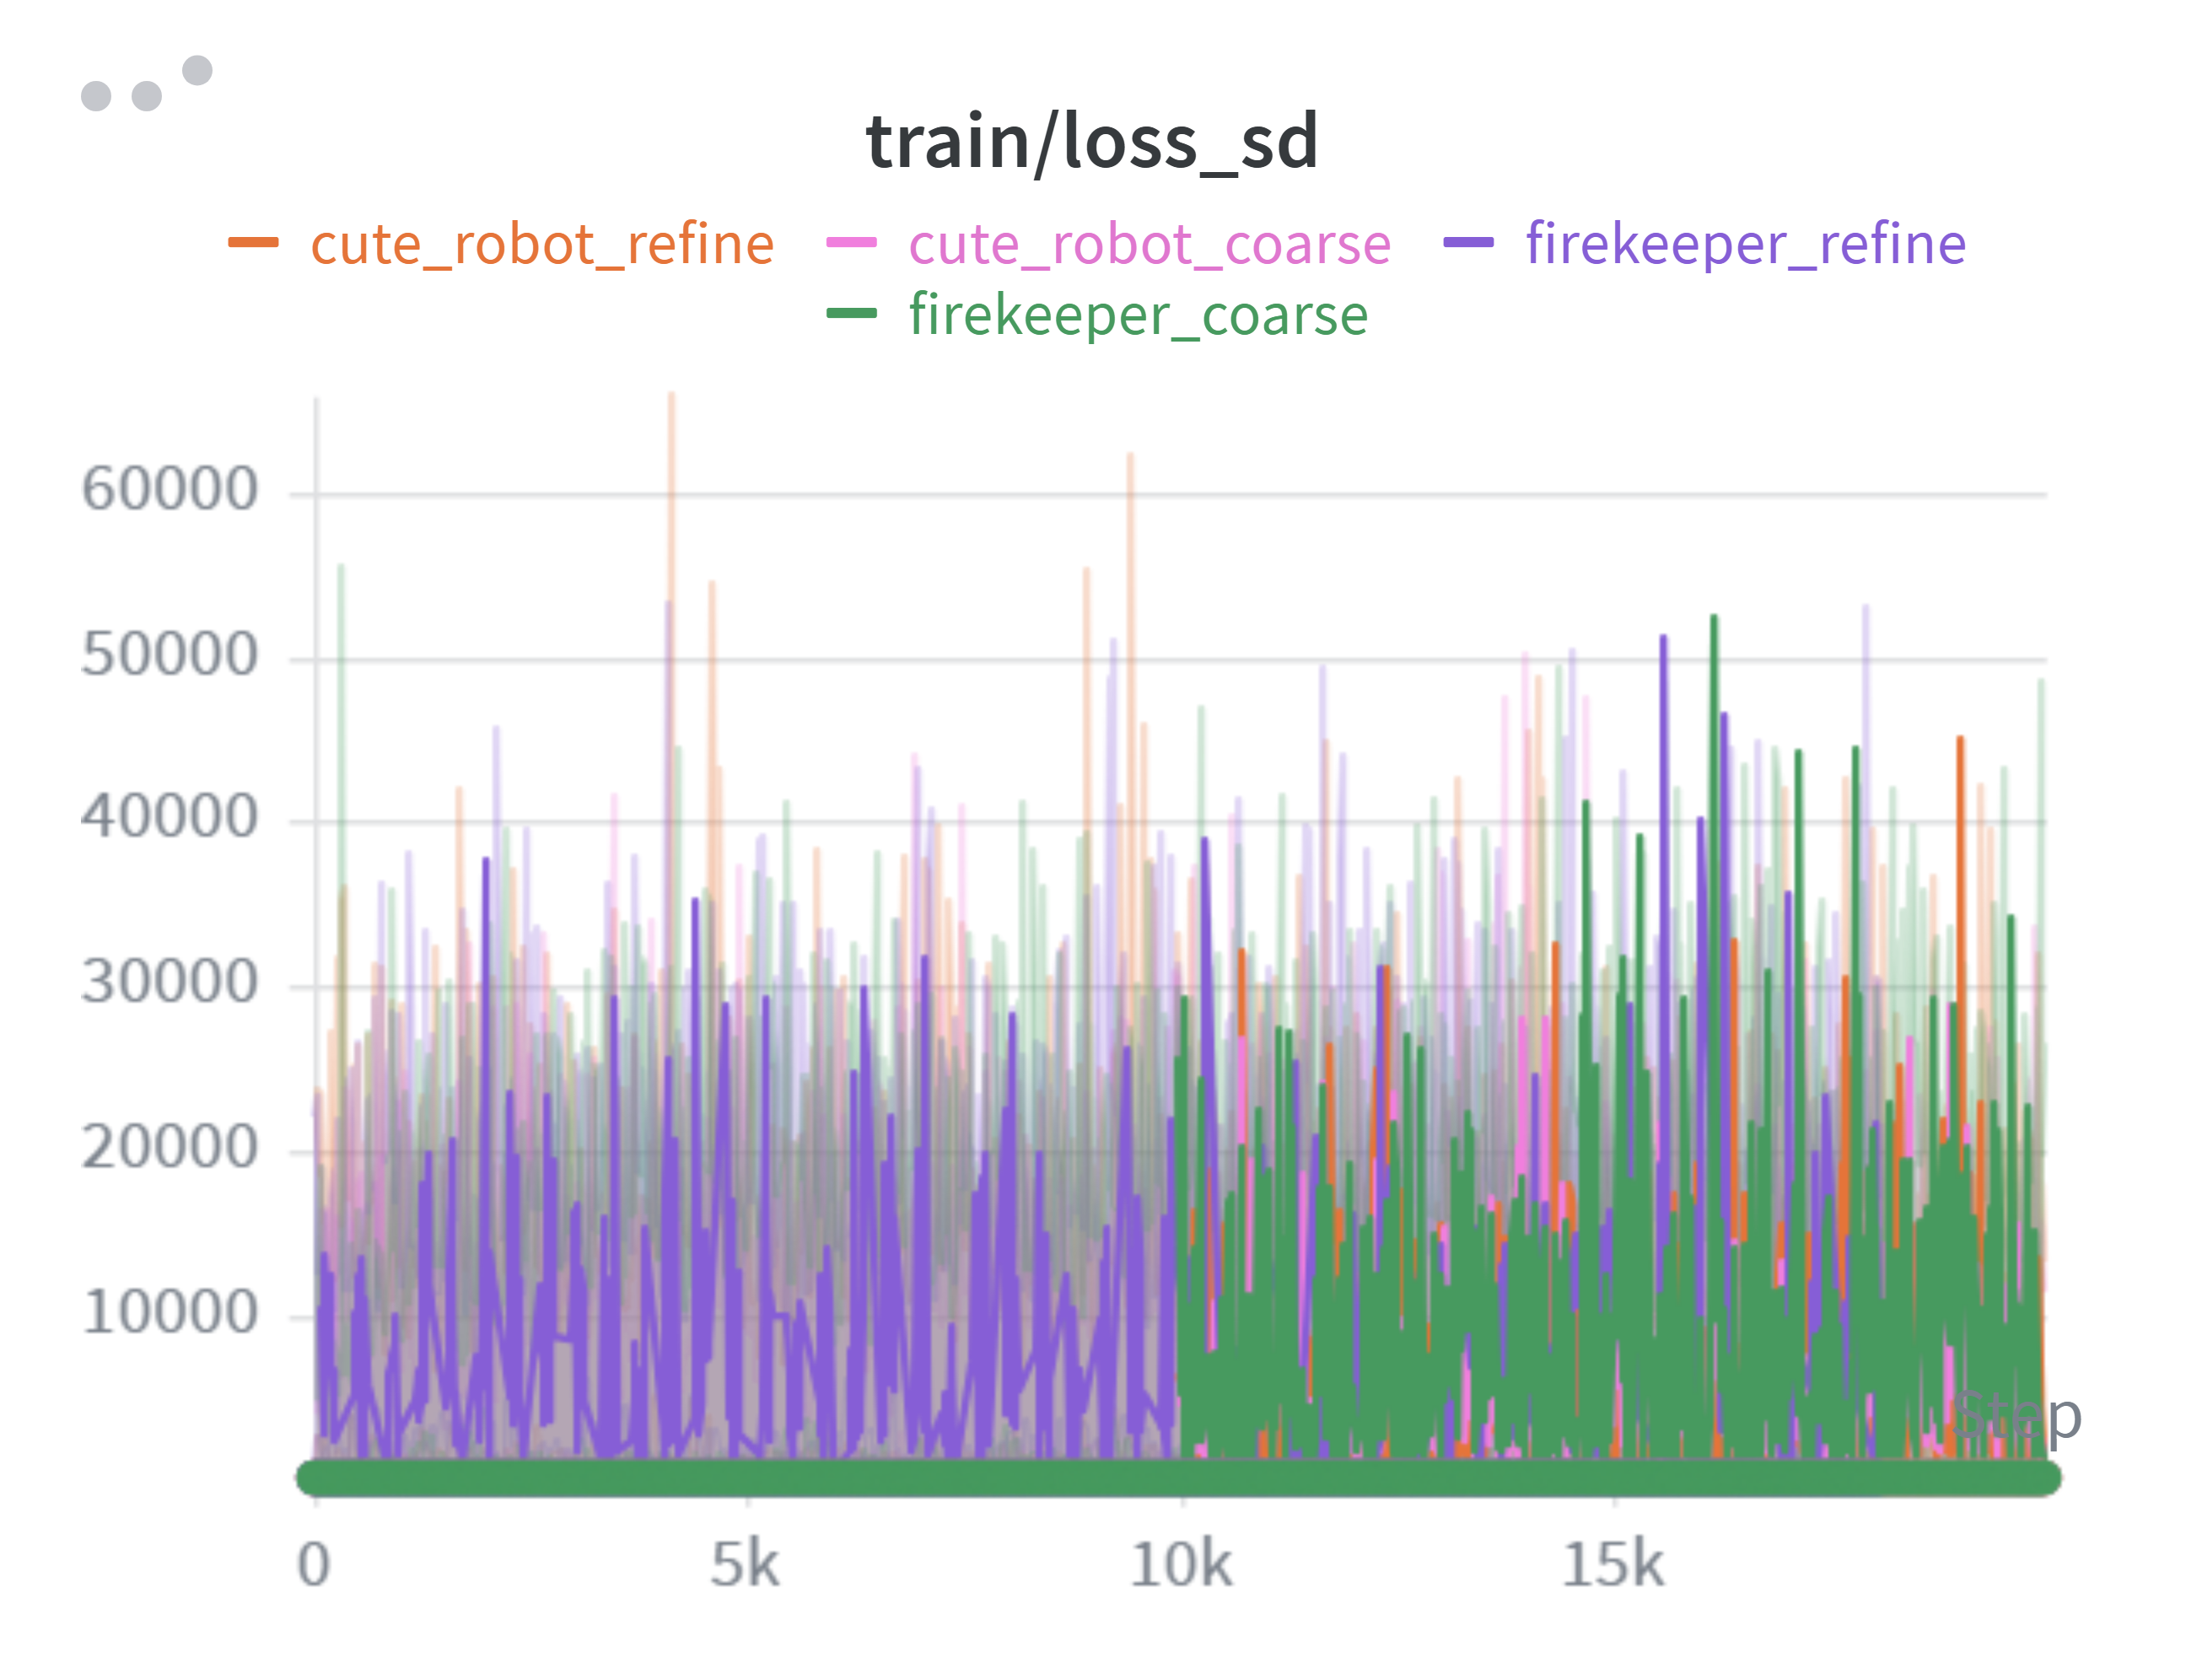
\includegraphics[width=\linewidth]{figures/task1/objectC/losses/loss_sd.png}
		\caption{SDS loss}
	\end{subfigure}
	\hfill
	\begin{subfigure}[t]{0.32\textwidth}
		\centering
		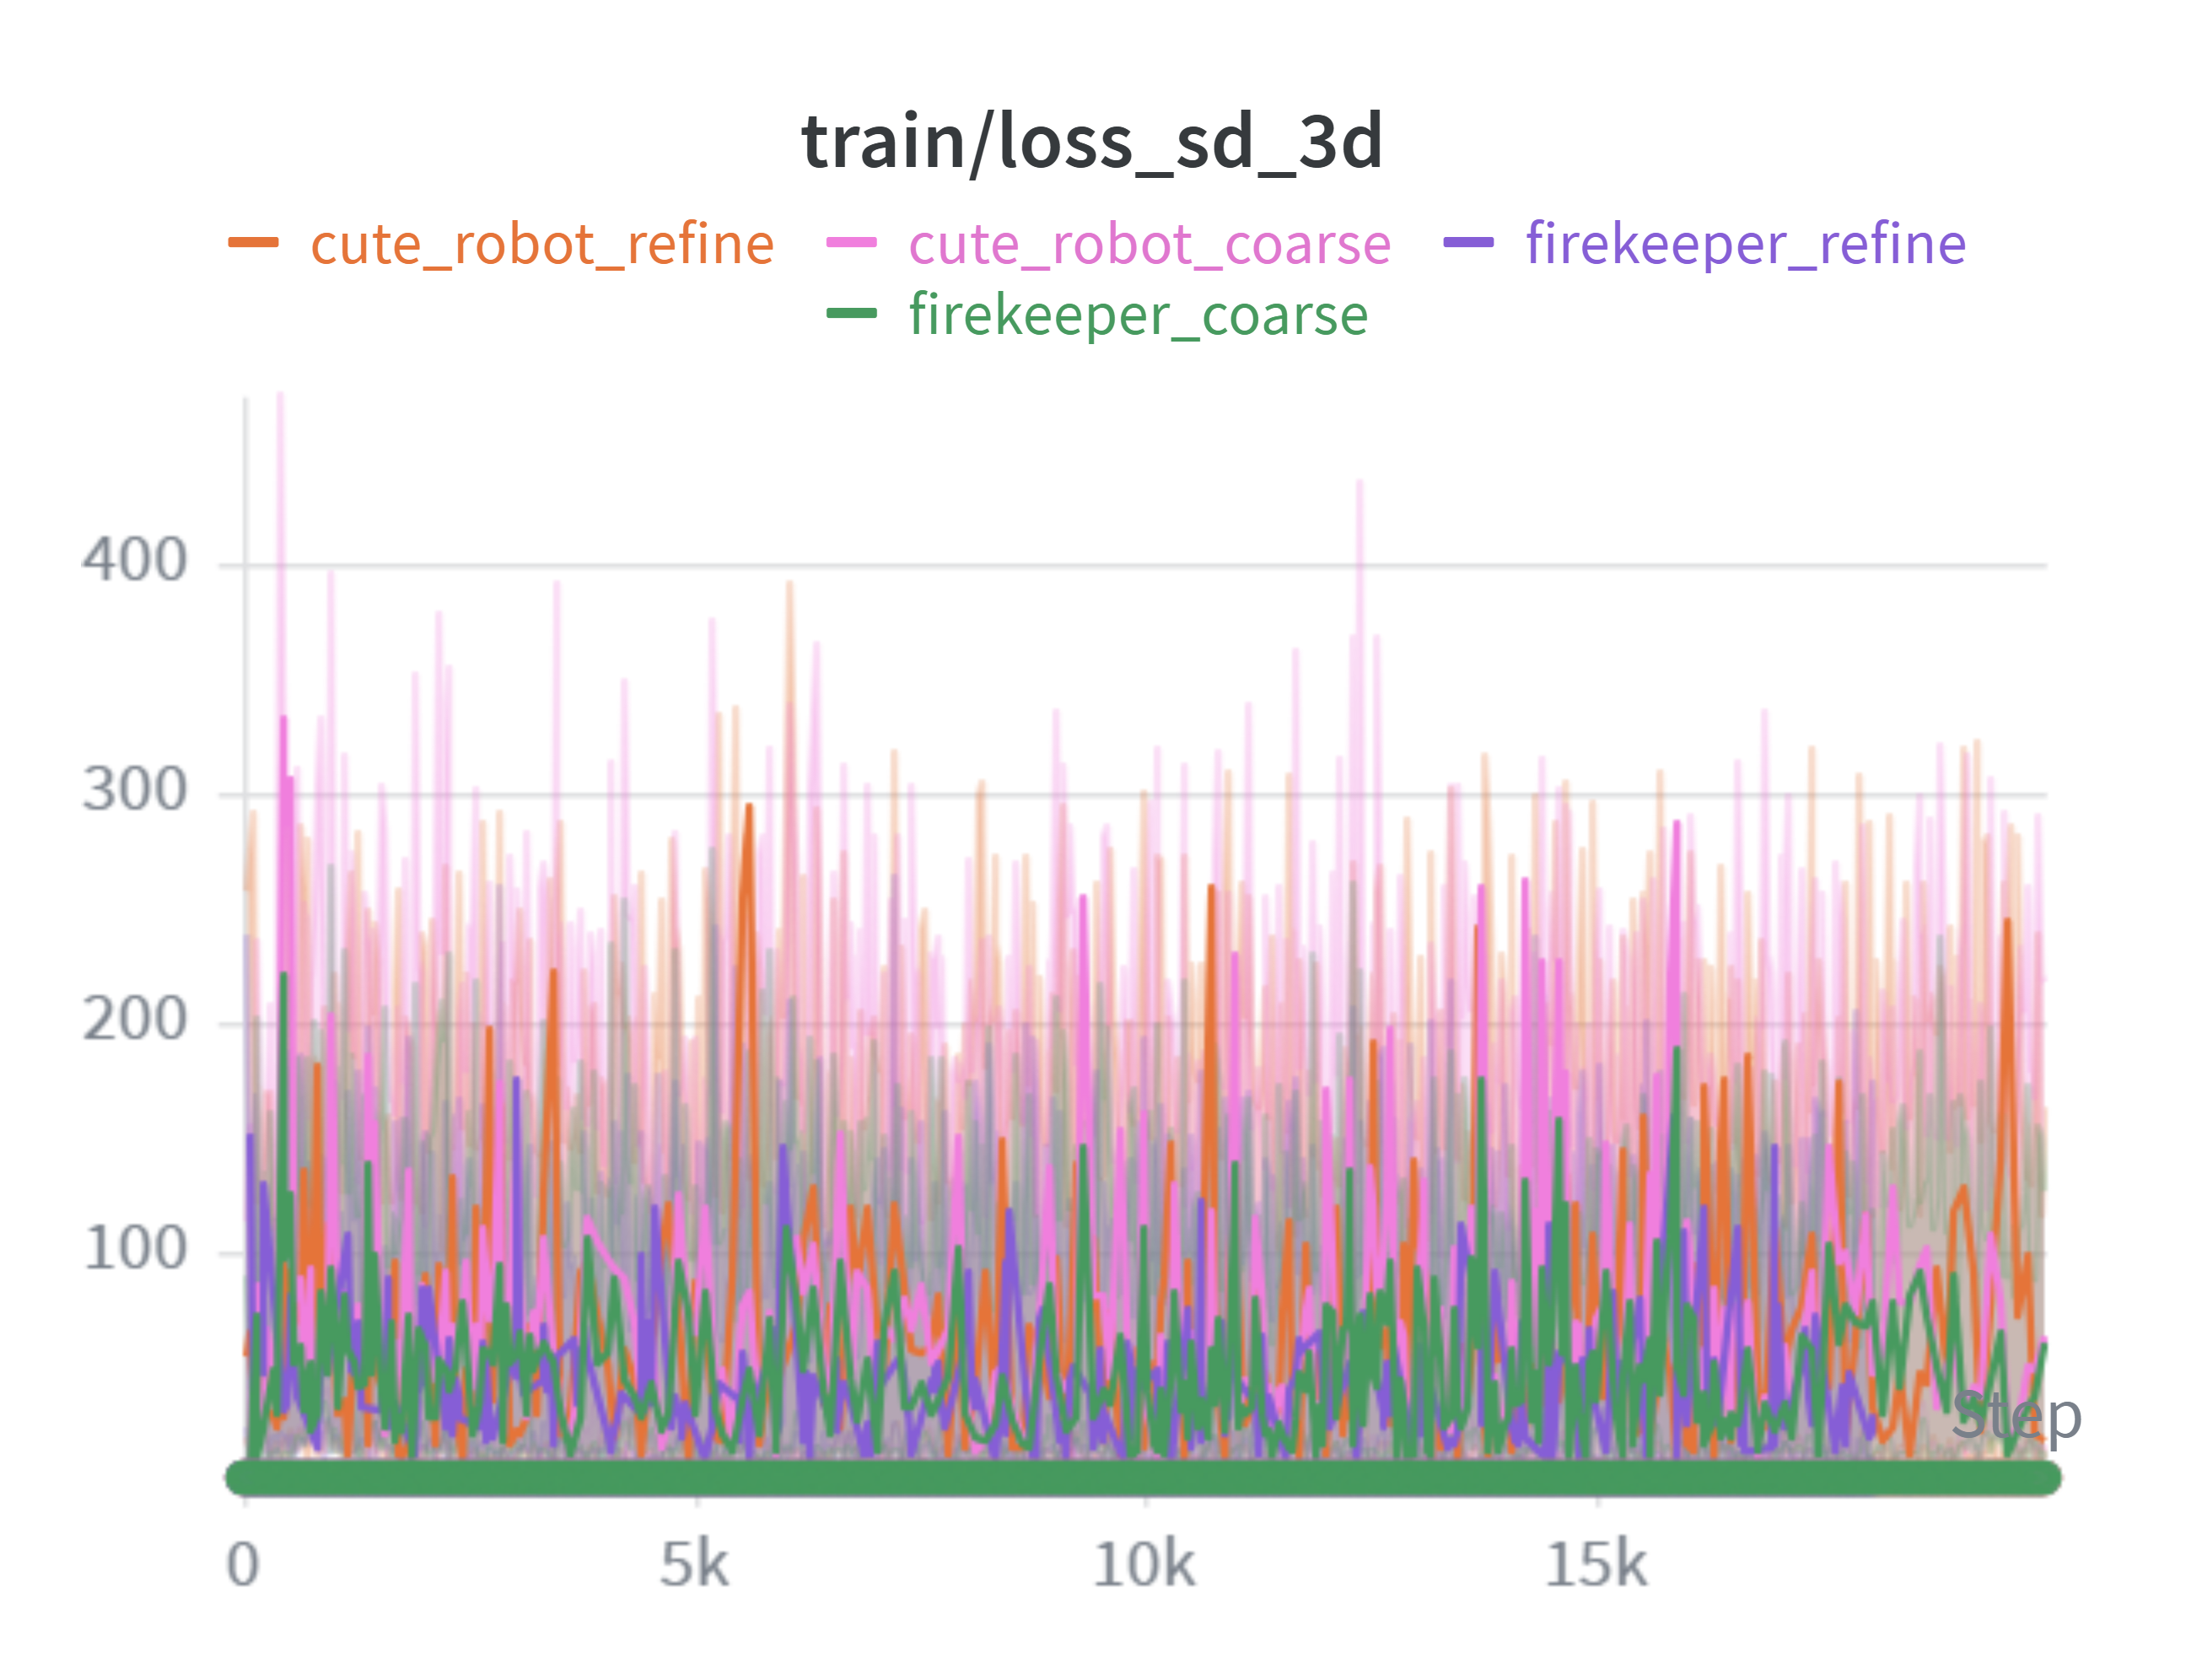
\includegraphics[width=\linewidth]{figures/task1/objectC/losses/loss_sd_3d.png}
		\caption{3D SDS loss}
	\end{subfigure}
	\hfill
	\begin{subfigure}[t]{0.32\textwidth}
		\centering
		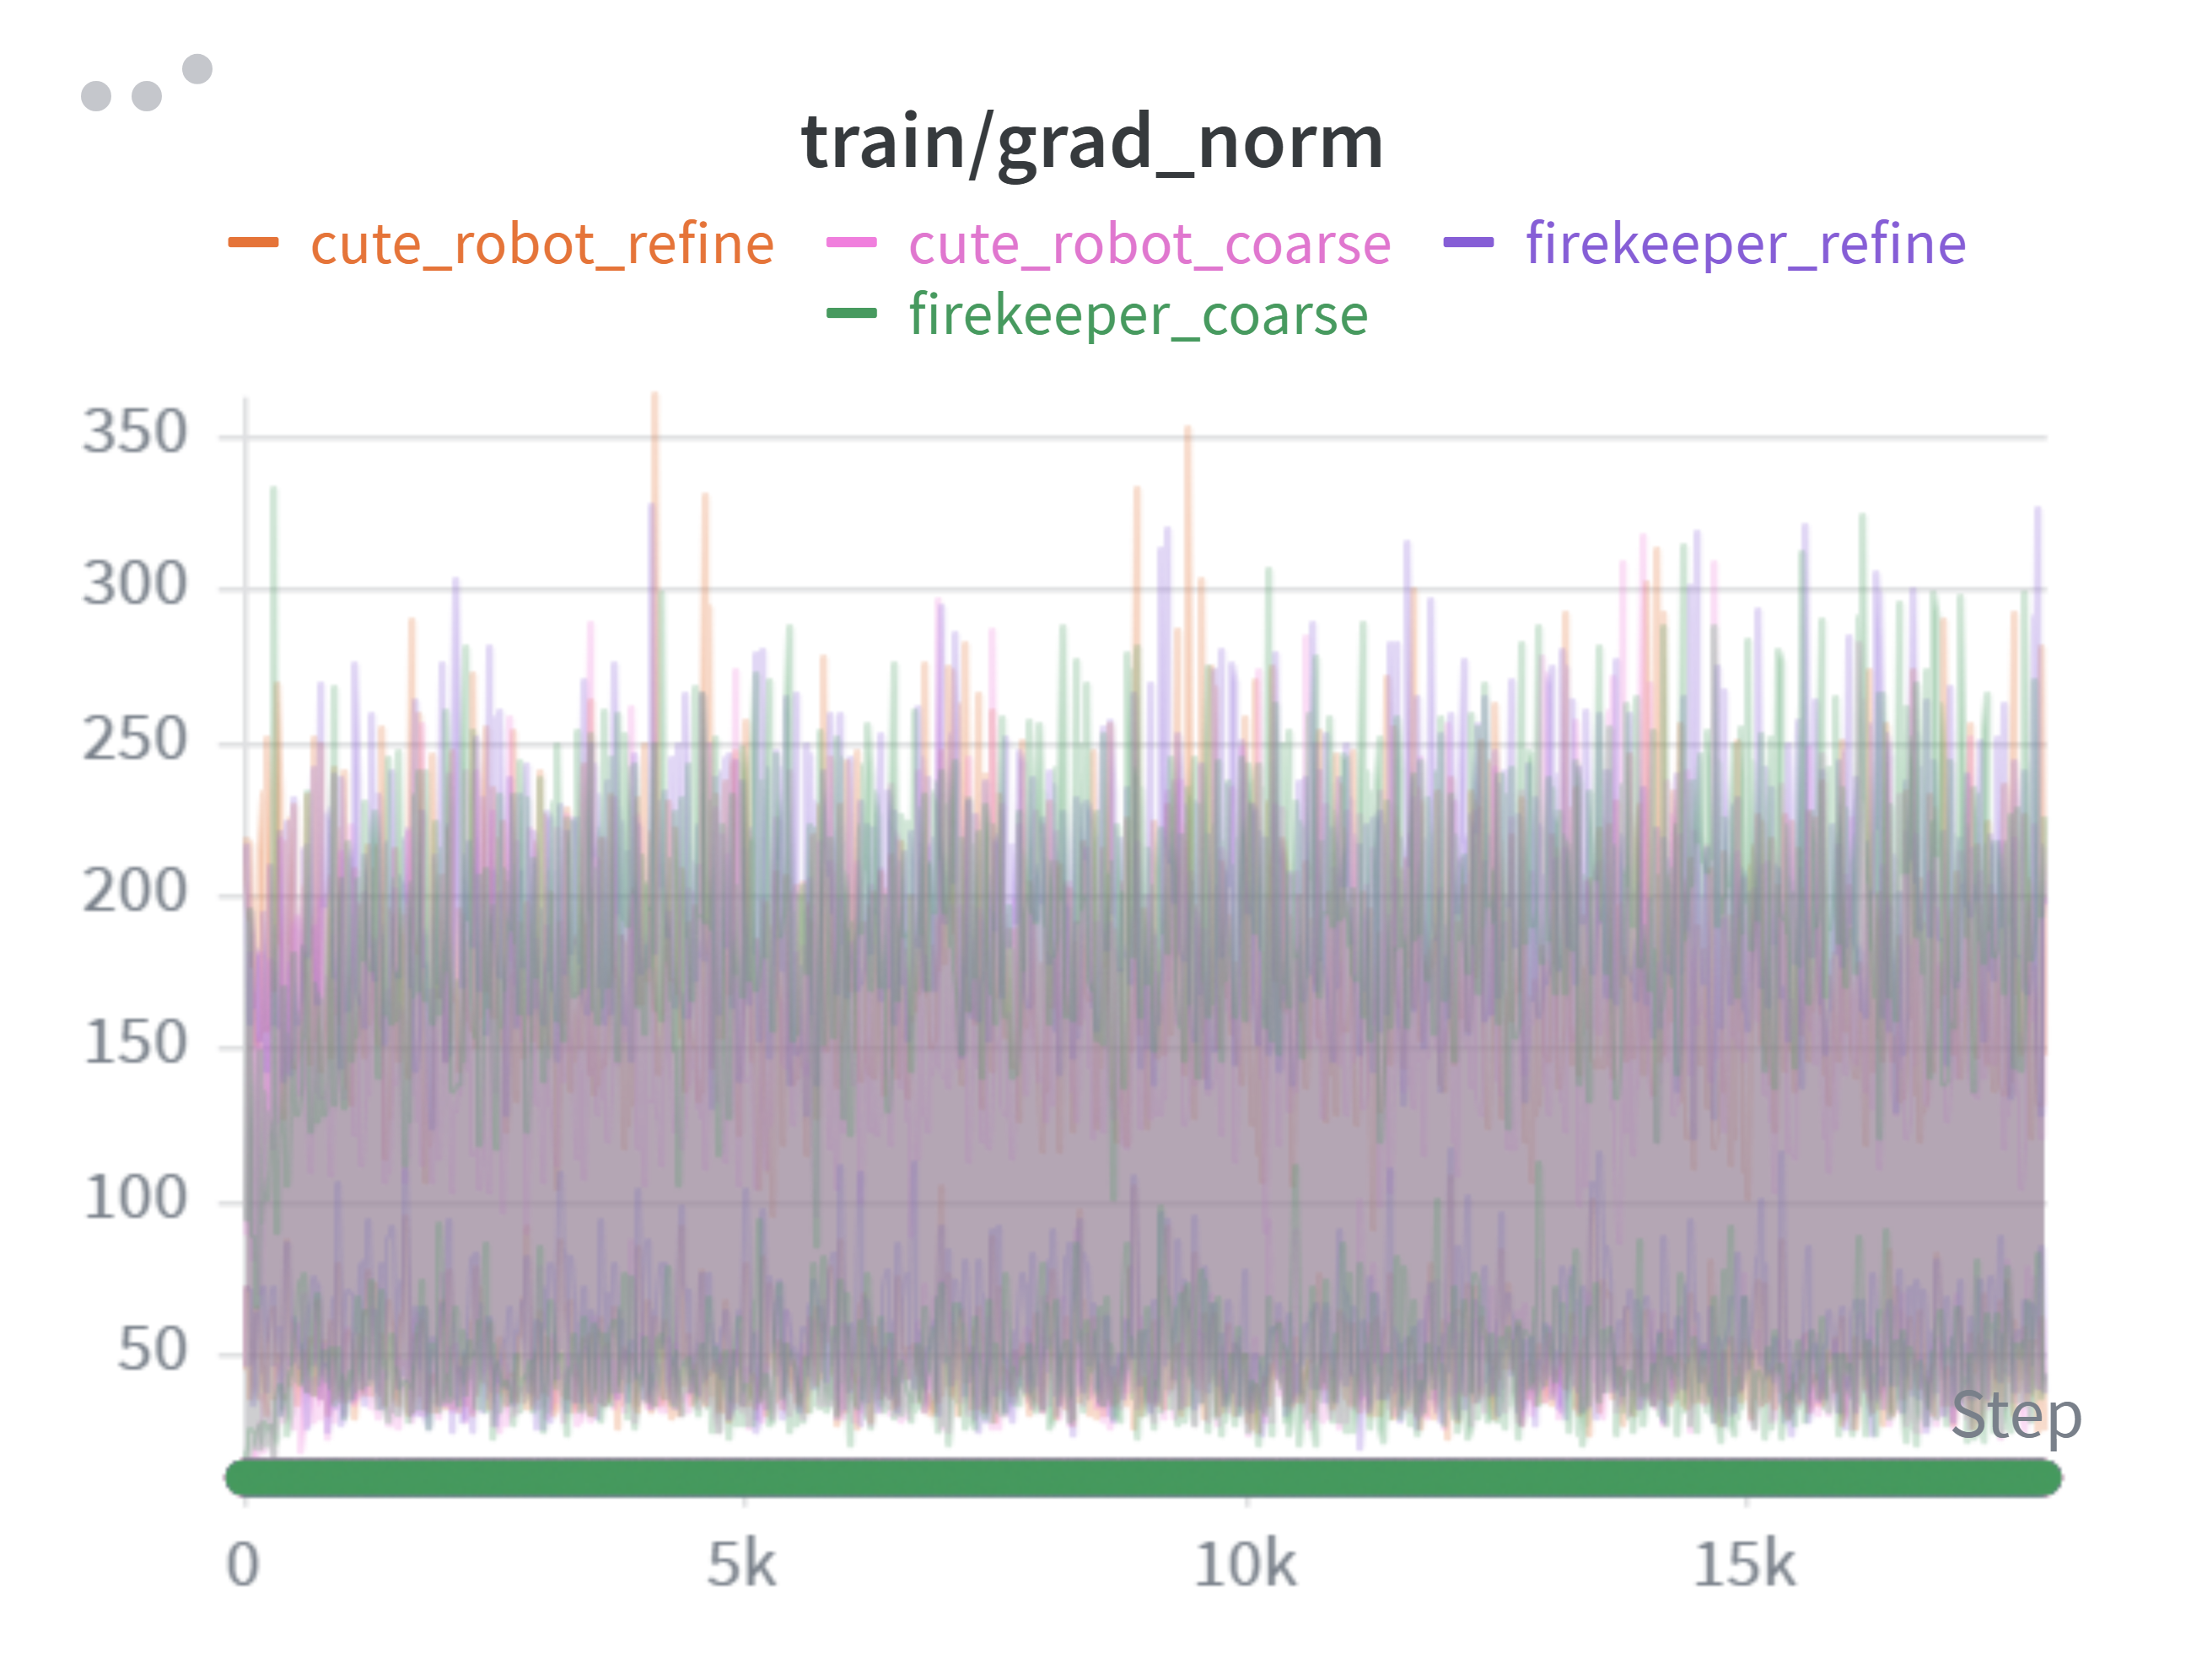
\includegraphics[width=\linewidth]{figures/task1/objectC/losses/grad_norm.png}
		\caption{Gradient norm}
	\end{subfigure}
	
	\vspace{0.5cm}
	
	%==================== 第二组：Regularization ====================
	\begin{subfigure}[t]{0.32\textwidth}
		\centering
		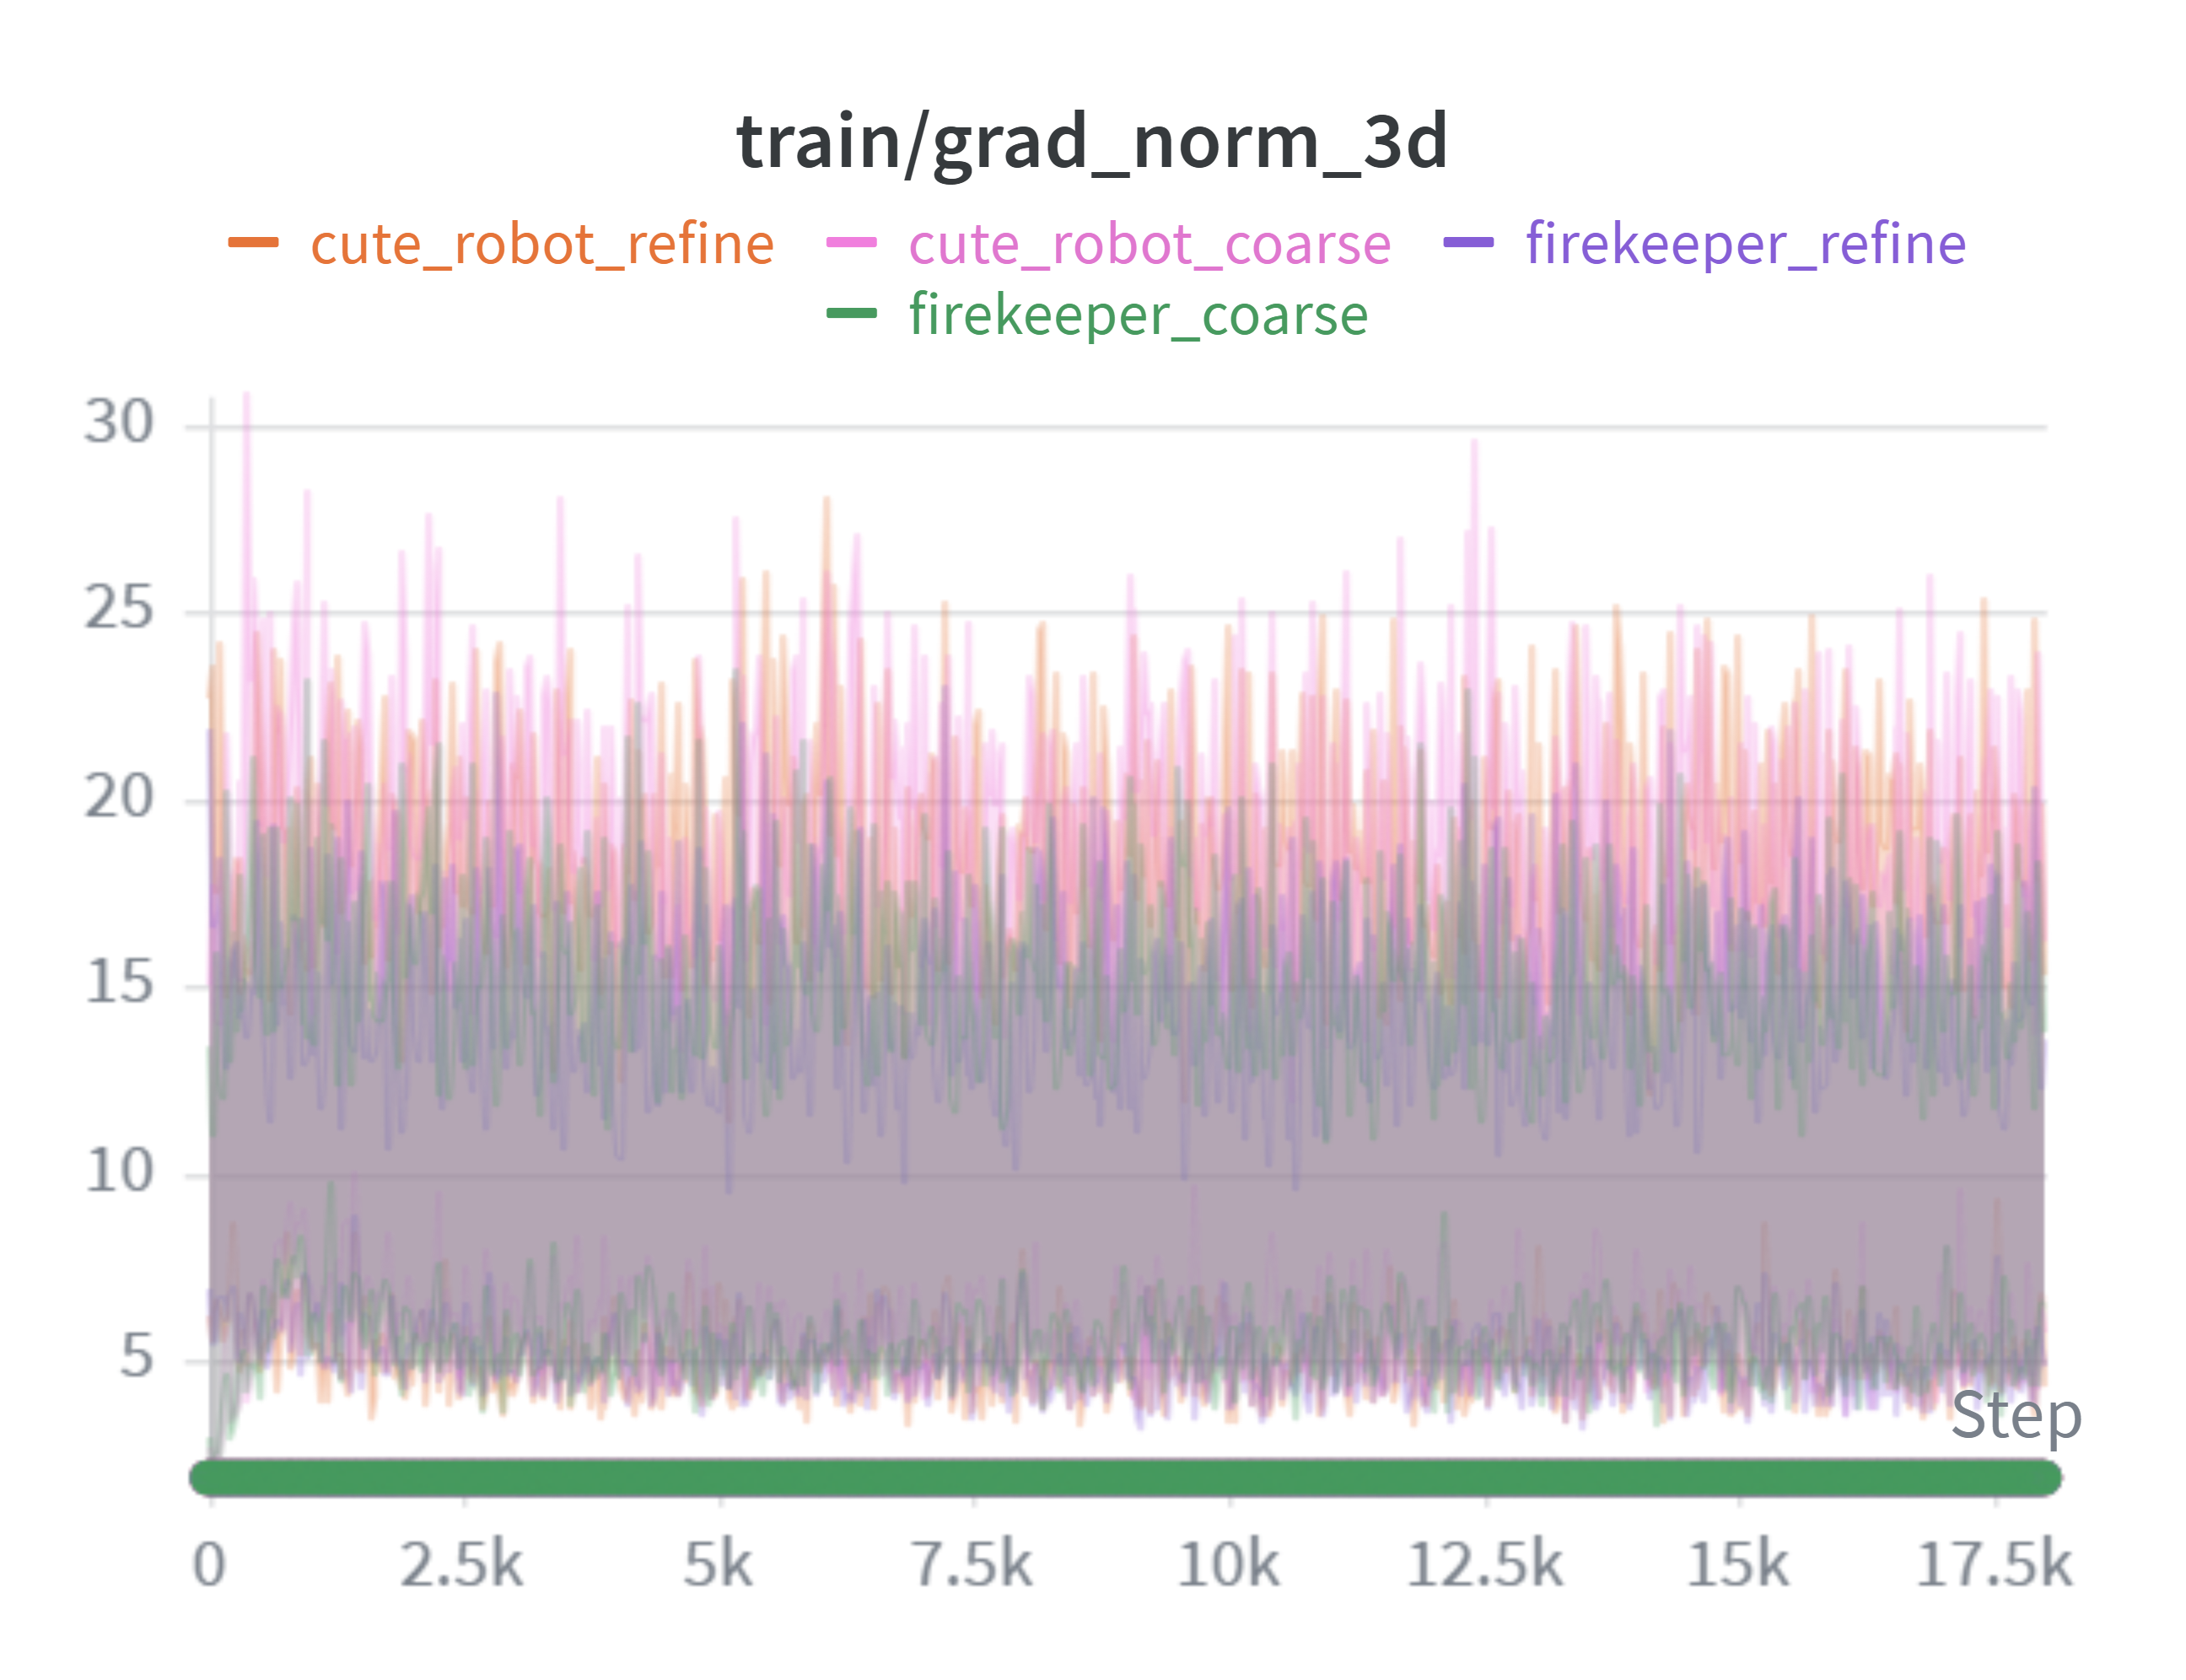
\includegraphics[width=\linewidth]{figures/task1/objectC/losses/grad_norm_3d.png}
		\caption{3D gradient norm}
	\end{subfigure}
	\hfill
	\begin{subfigure}[t]{0.32\textwidth}
		\centering
		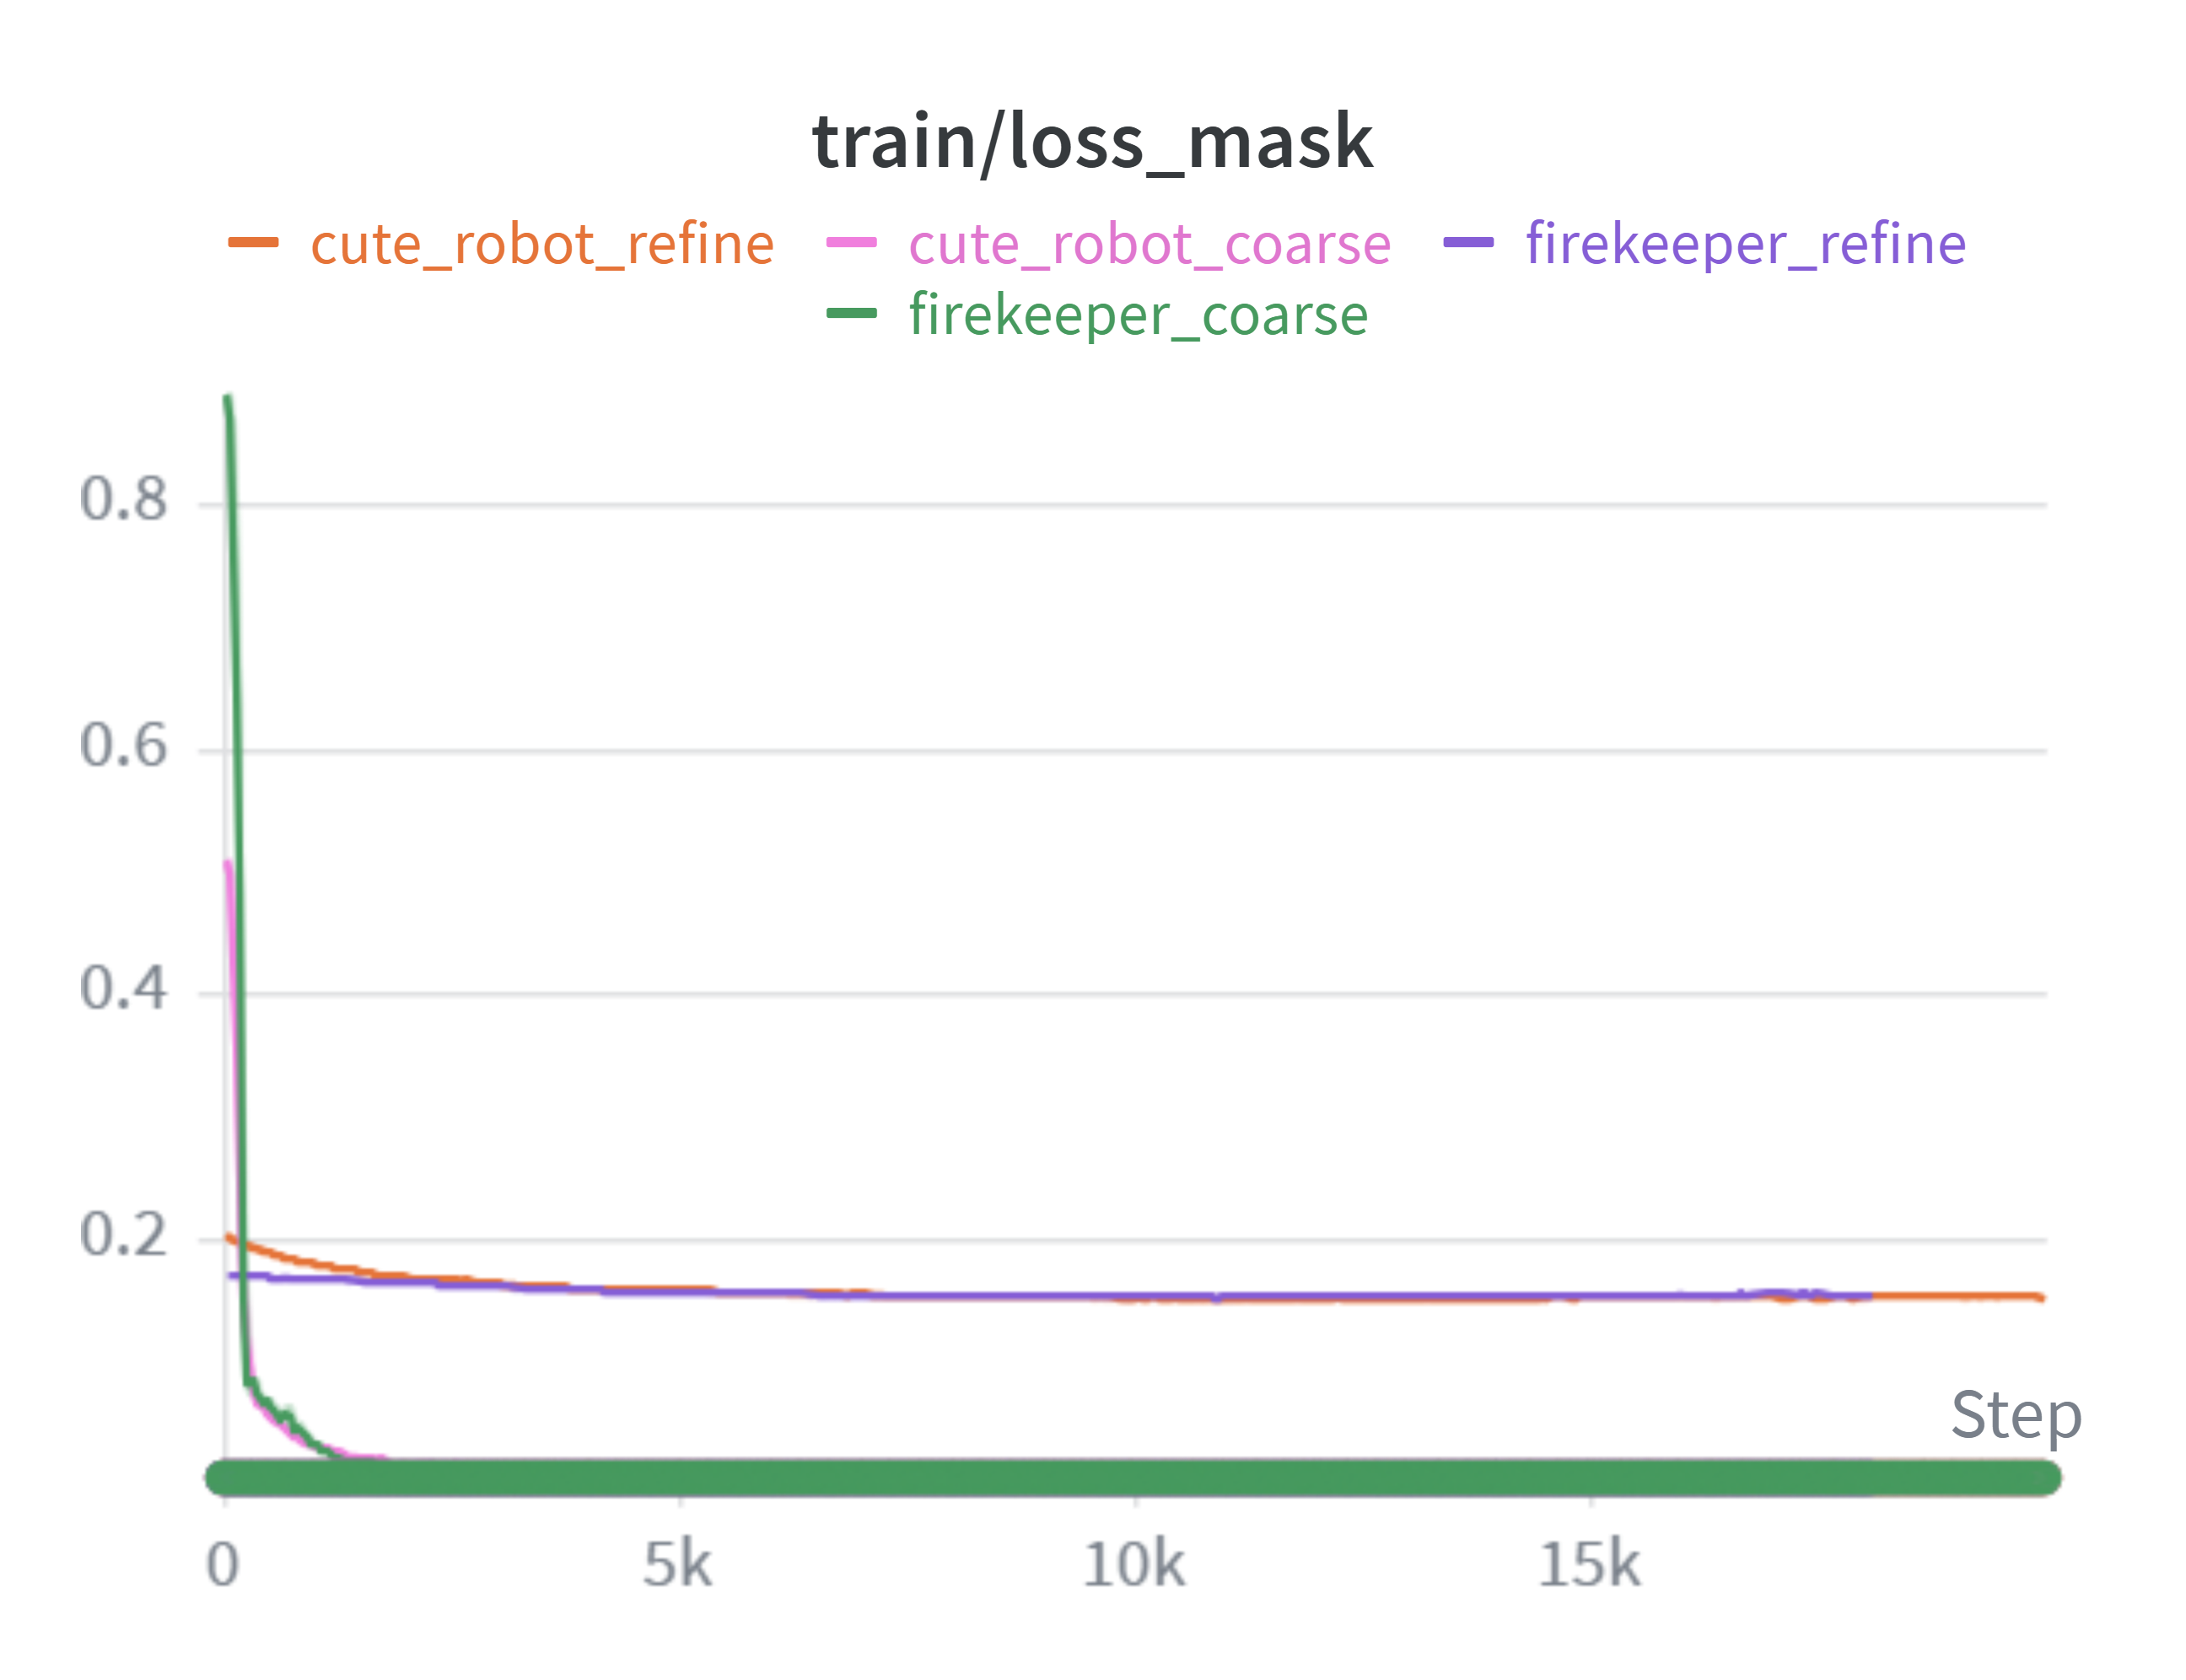
\includegraphics[width=\linewidth]{figures/task1/objectC/losses/loss_mask.png}
		\caption{Mask loss}
	\end{subfigure}
	\hfill
	\begin{subfigure}[t]{0.32\textwidth}
		\centering
		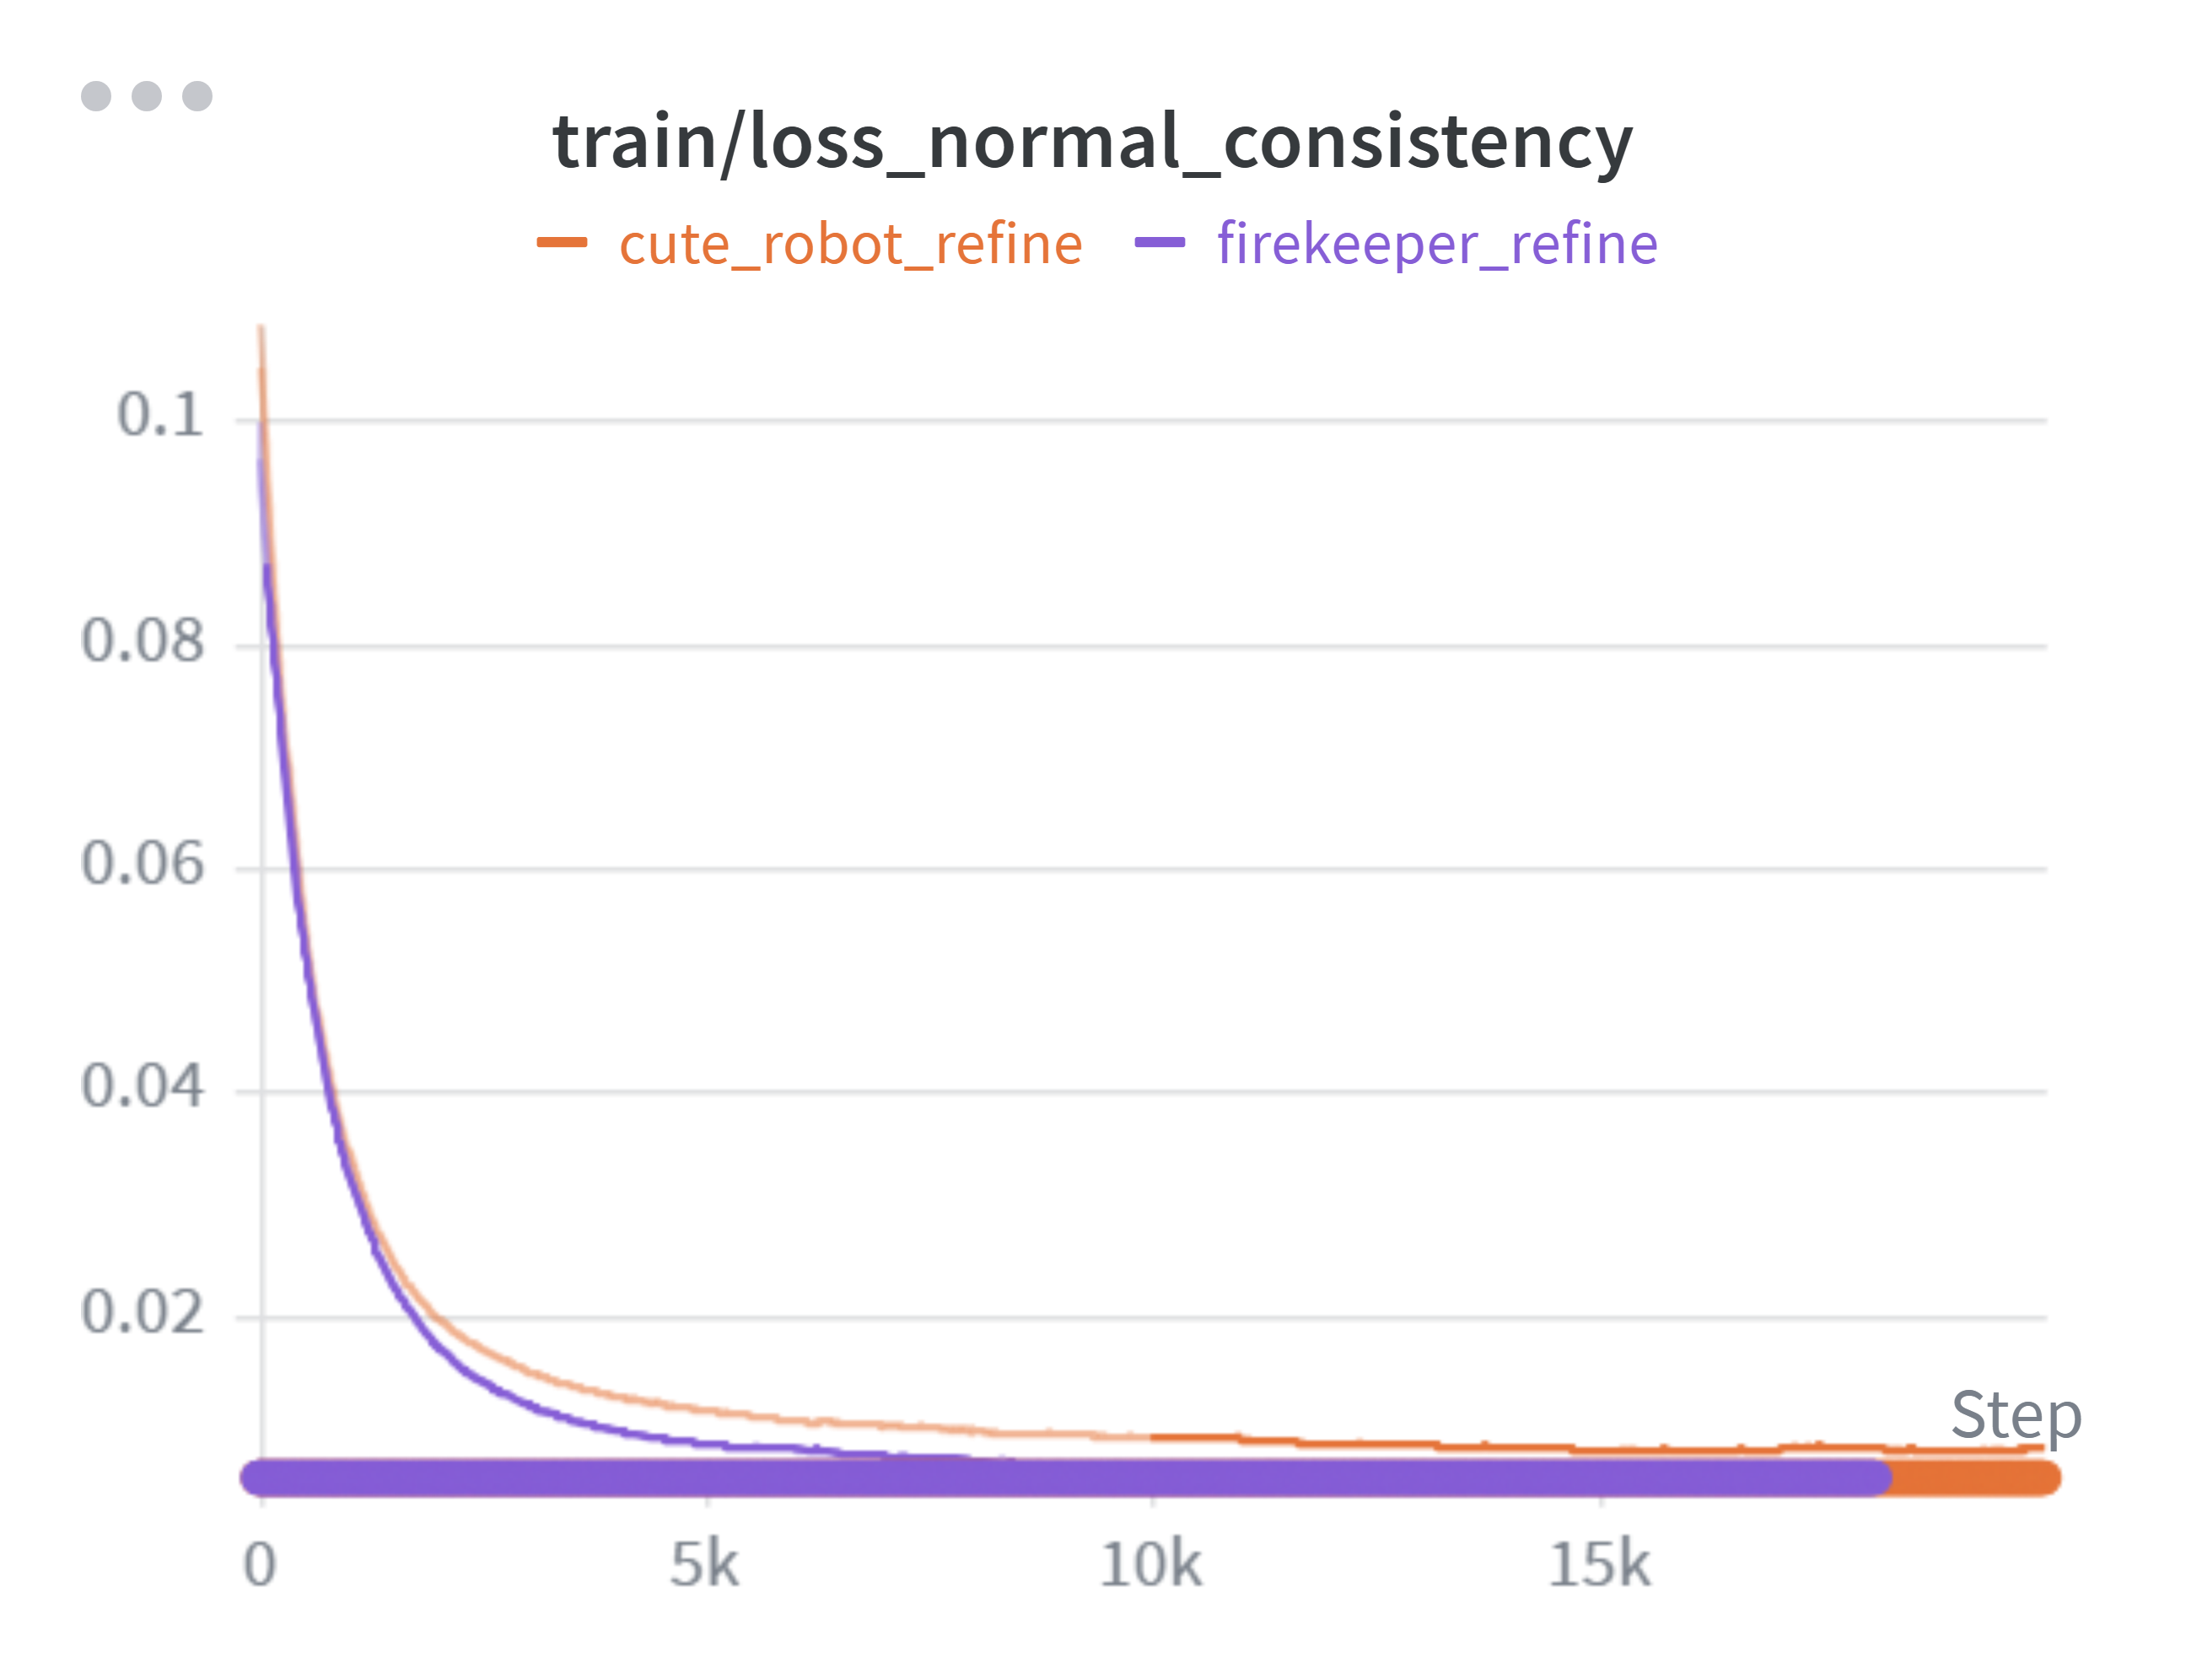
\includegraphics[width=\linewidth]{figures/task1/objectC/losses/loss_normal_consistency.png}
		\caption{Normal consistency loss}
	\end{subfigure}
	
	\vspace{0.5cm}
	
	%==================== 第三组：Reconstruction ====================
	\begin{subfigure}[t]{0.45\textwidth}
		\centering
		
\includegraphics[width=\linewidth]{figures/task1/objectC/losses/rgb_loss.png}
		\caption{RGB reconstruction loss}
	\end{subfigure}
	
	\caption{Training losses and optimization statistics for Object C.}
	\label{fig:objectC_losses}
\end{figure*}


We can see that the visualization results of both models have good and smooth shape and color distribution.

As for the training dynamics, here are our analysis:

Opaque Loss demonstrates a similar pattern as Object B, but with no obvious shakes. This may because the picture offers enough geometry features for the model so that it can easily build the rough but accurate outfit.

Sparsity Loss has a similar behavior as Object B.


The SDS Loss and 3D SDS Loss exhibit large fluctuations and high variance, which can be interpreted similarly as the SDS loss of Object B.

The gradient norm remains within a stable range overall. Although there are shakes, no persistent gradient explosion or vanishing occurs. This indicates that the training process is generally stable and the optimizer can effectively control parameter updates.

The Mask Loss decreases rapidly in the early stage of training and gradually converges to a low value, indicating that the model can quickly learn the separation between foreground and background regions, which helps improve the accuracy of geometric structures.

The Normal Consistency Loss exhibits a clear rapid decay trend, indicating that the normal consistency of the mesh surface continuously increases. This constraint effectively reduces local noise and discontinuous surfaces, making the generated results smoother.

The RGB Reconstruction Loss decreases and finally stabilizes, demonstrating that the model's texture and color reconstruction capabilities are continuously improving, and the difference between the rendered results and the target image keeps decreasing.


\subsection{Background Scene Visualization}
In this section, 185 pictures of garden(picking $\frac{1}{4}$ of the original resolution for efficiency) are trained. It takes about \textbf{1:12:42hour} to extract pose with COLMAP and \textbf{19:30min}(20000 epochs) to train.

One of the original pictures and the rendering results are as follow:
\begin{figure}[H]
	\centering
	

	\begin{subfigure}{0.25\textwidth}
		\centering
		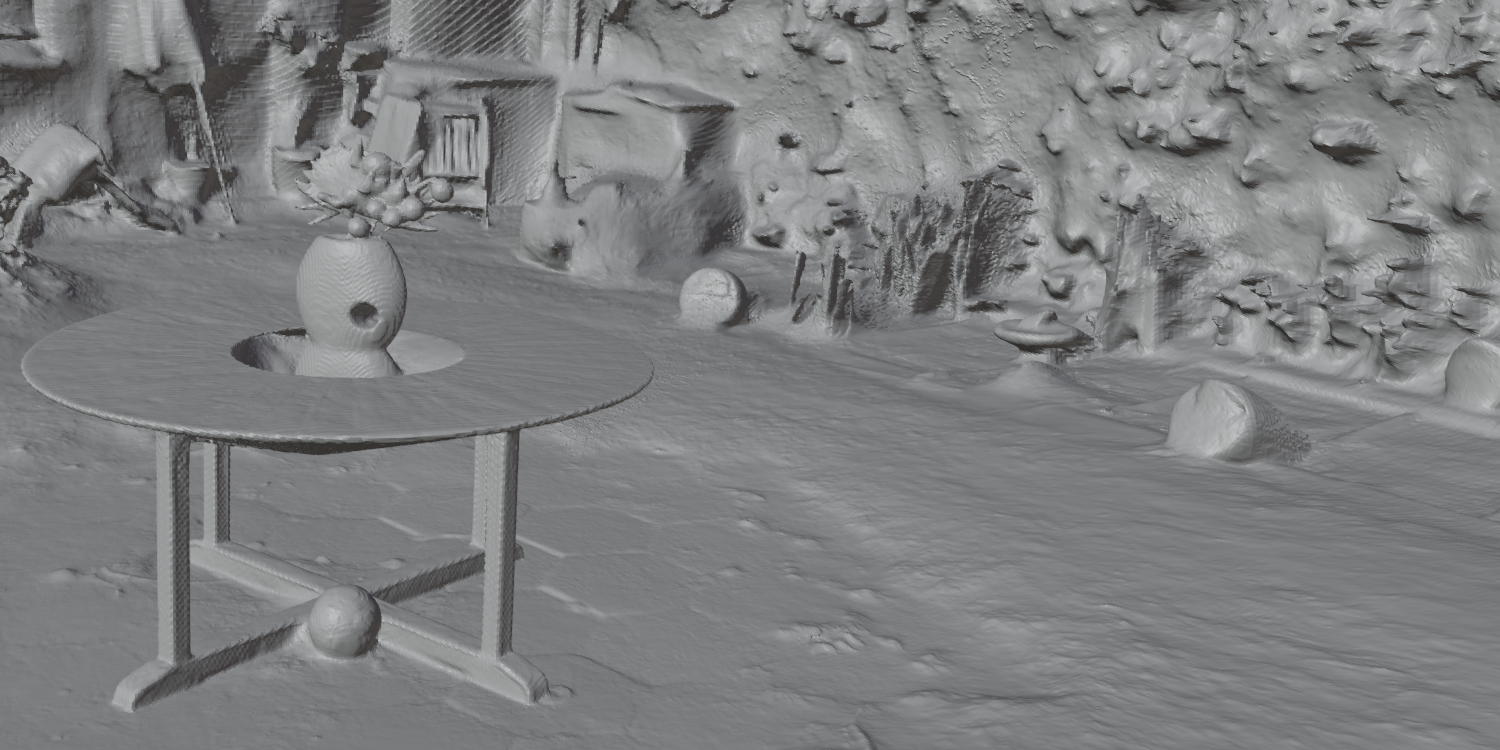
\includegraphics[width=\linewidth]{figures/task1/background/garden_mesh.png}
		\caption{Garden Mesh}
	\end{subfigure}
	\hfill
	\begin{subfigure}{0.25\textwidth}
		\centering
		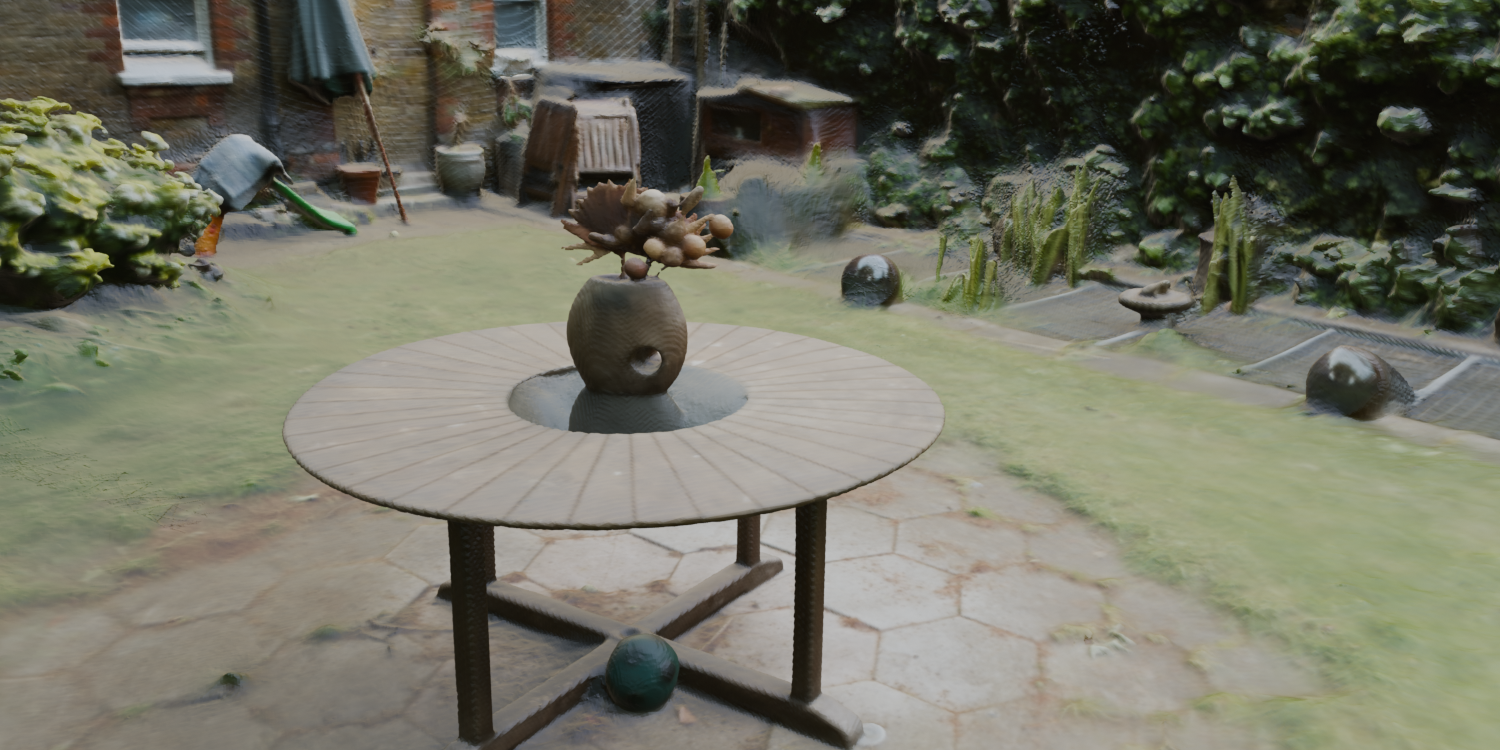
\includegraphics[width=\linewidth]{figures/task1/background/garden_color.png}
		\caption{Garden Color}
	\end{subfigure}
	\hfill
	\begin{subfigure}{0.25\textwidth}
		\centering
		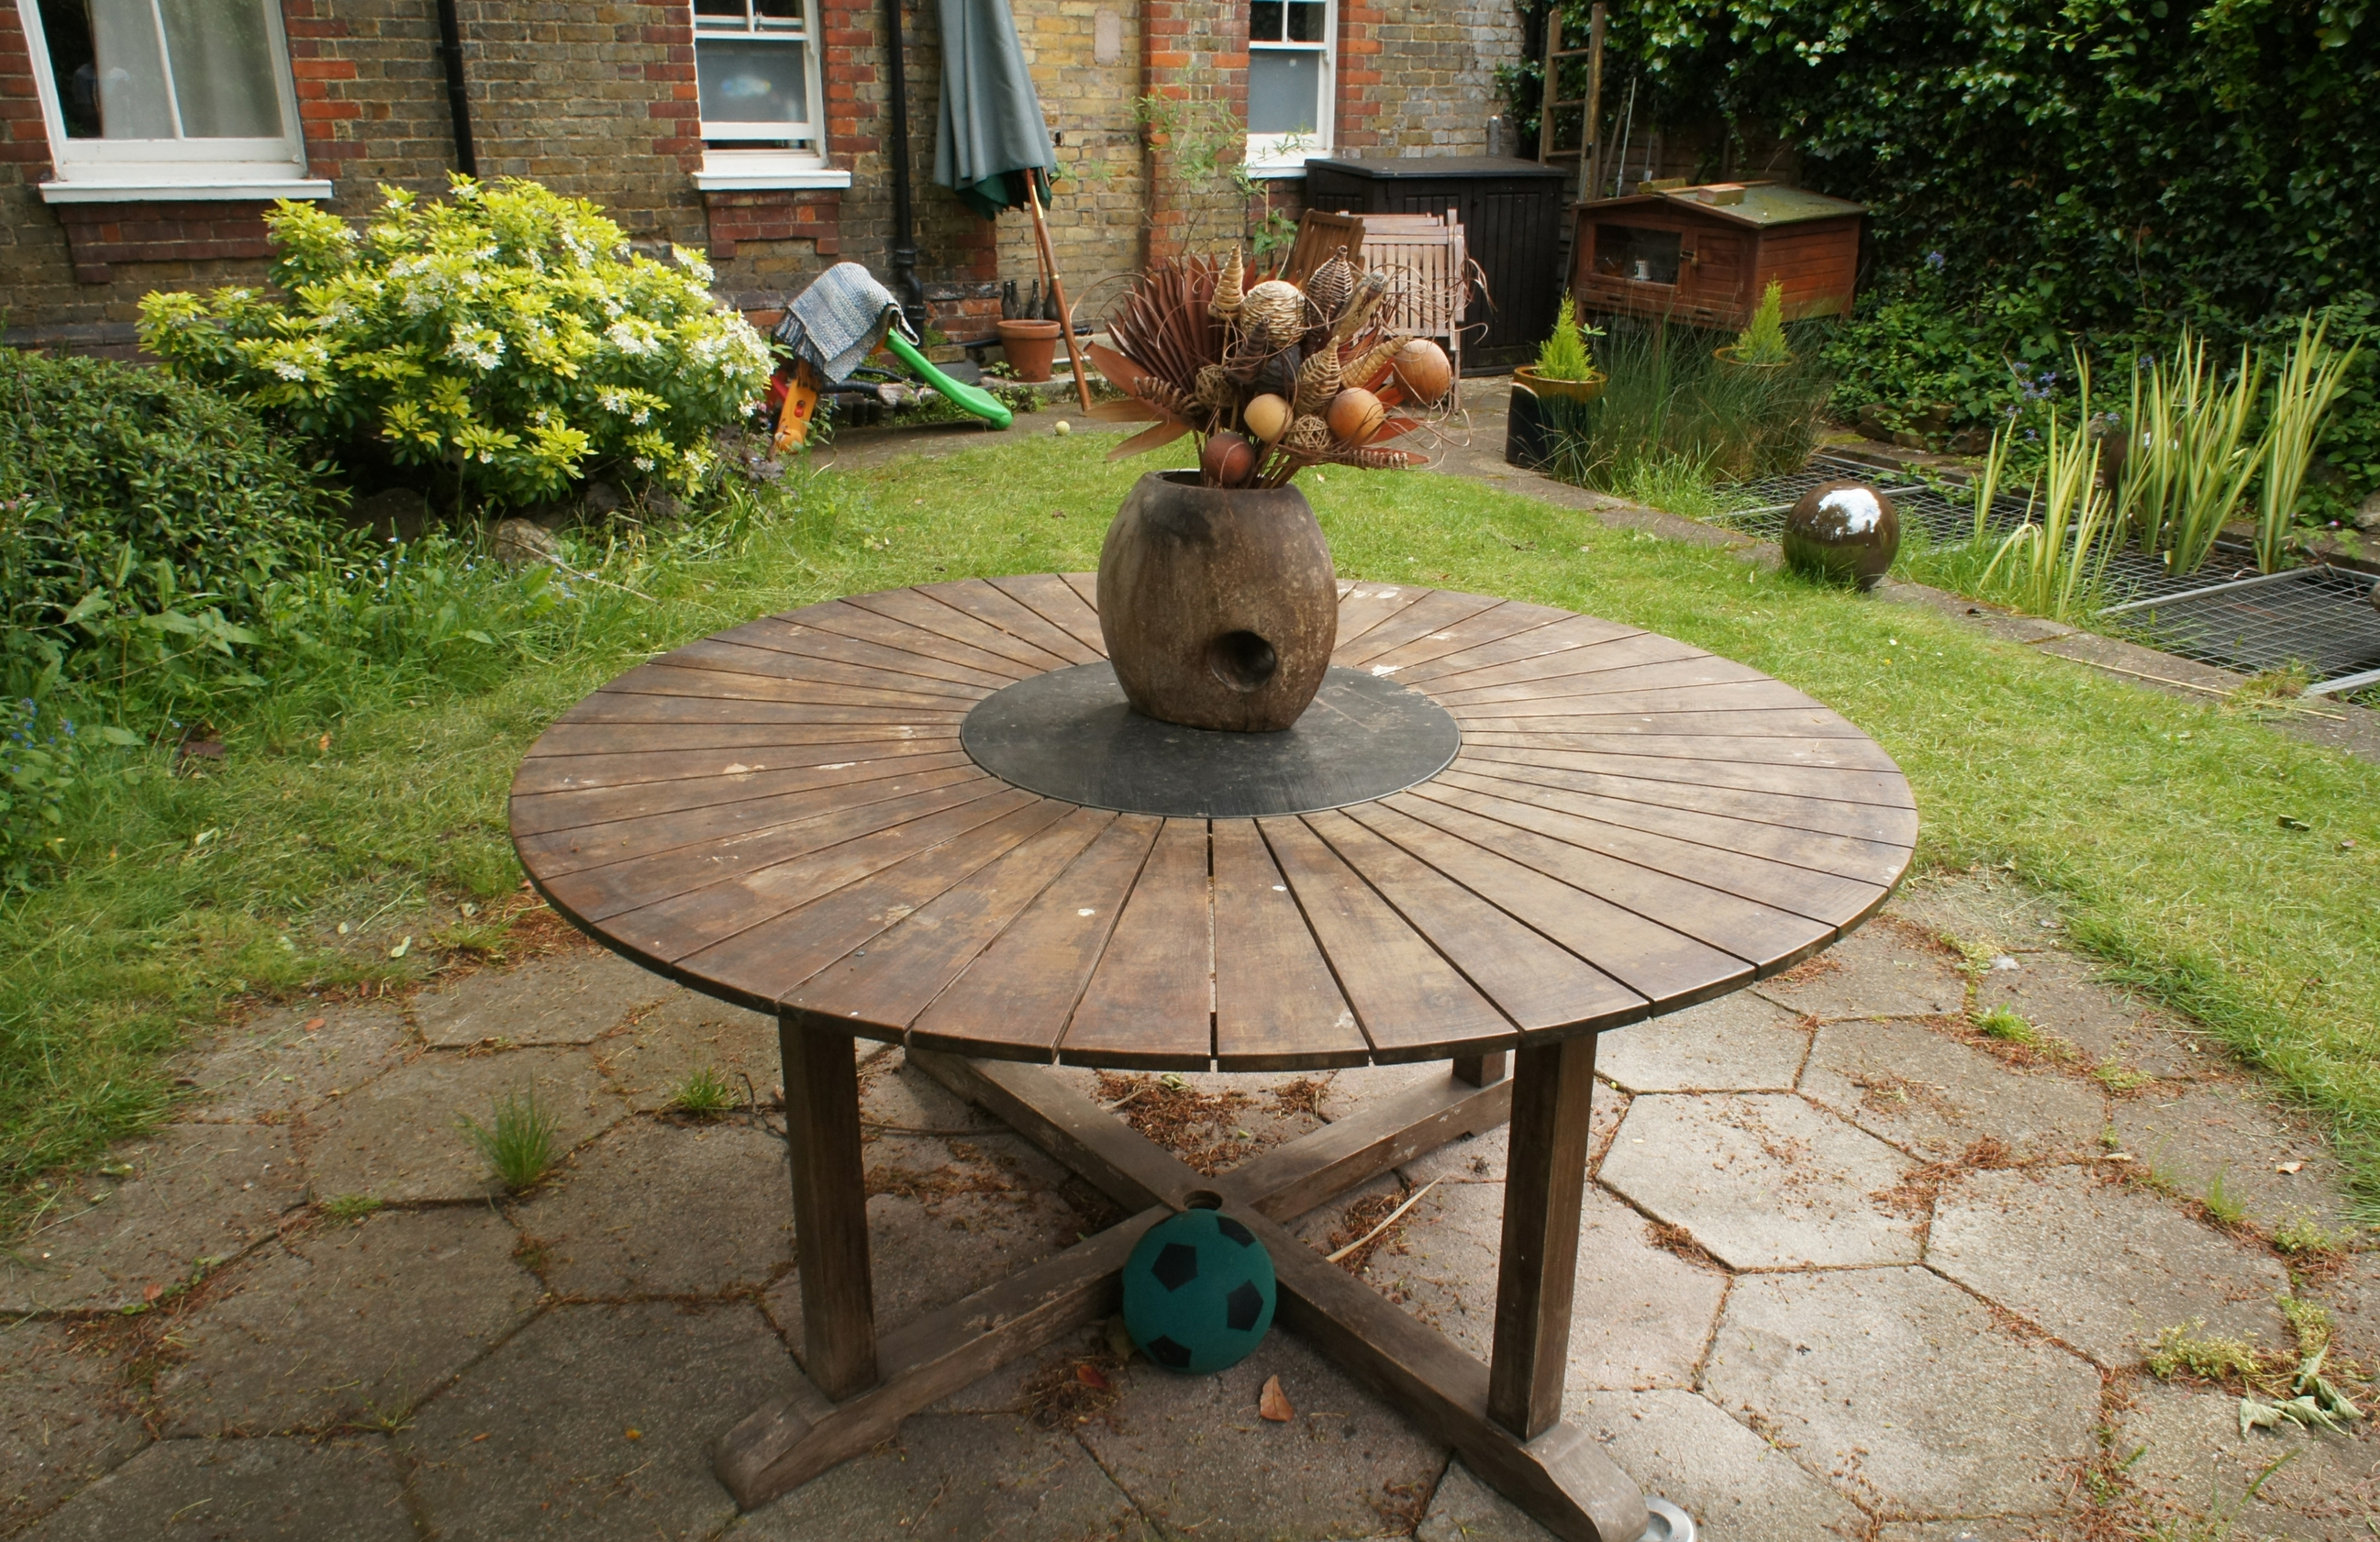
\includegraphics[width=\linewidth]{figures/task1/background/garden.jpg}
		\caption{Original Garden}
	\end{subfigure}
	
	\vspace{0.6cm}
	
	
\end{figure}
In this part, 2 meshes are exported(bounded and unbounded), where the unbounded mesh is in a form of a whole box. The box has an irregular outer shell and sky because these parts are not included in the images, while the rest of the model looks very good.


The detailed quality analysis will be shown later.



The training dynamics are as follow:

\begin{figure}[H]
	\centering
	
	% 第一行
	\begin{subfigure}{0.4\textwidth}
		\centering
		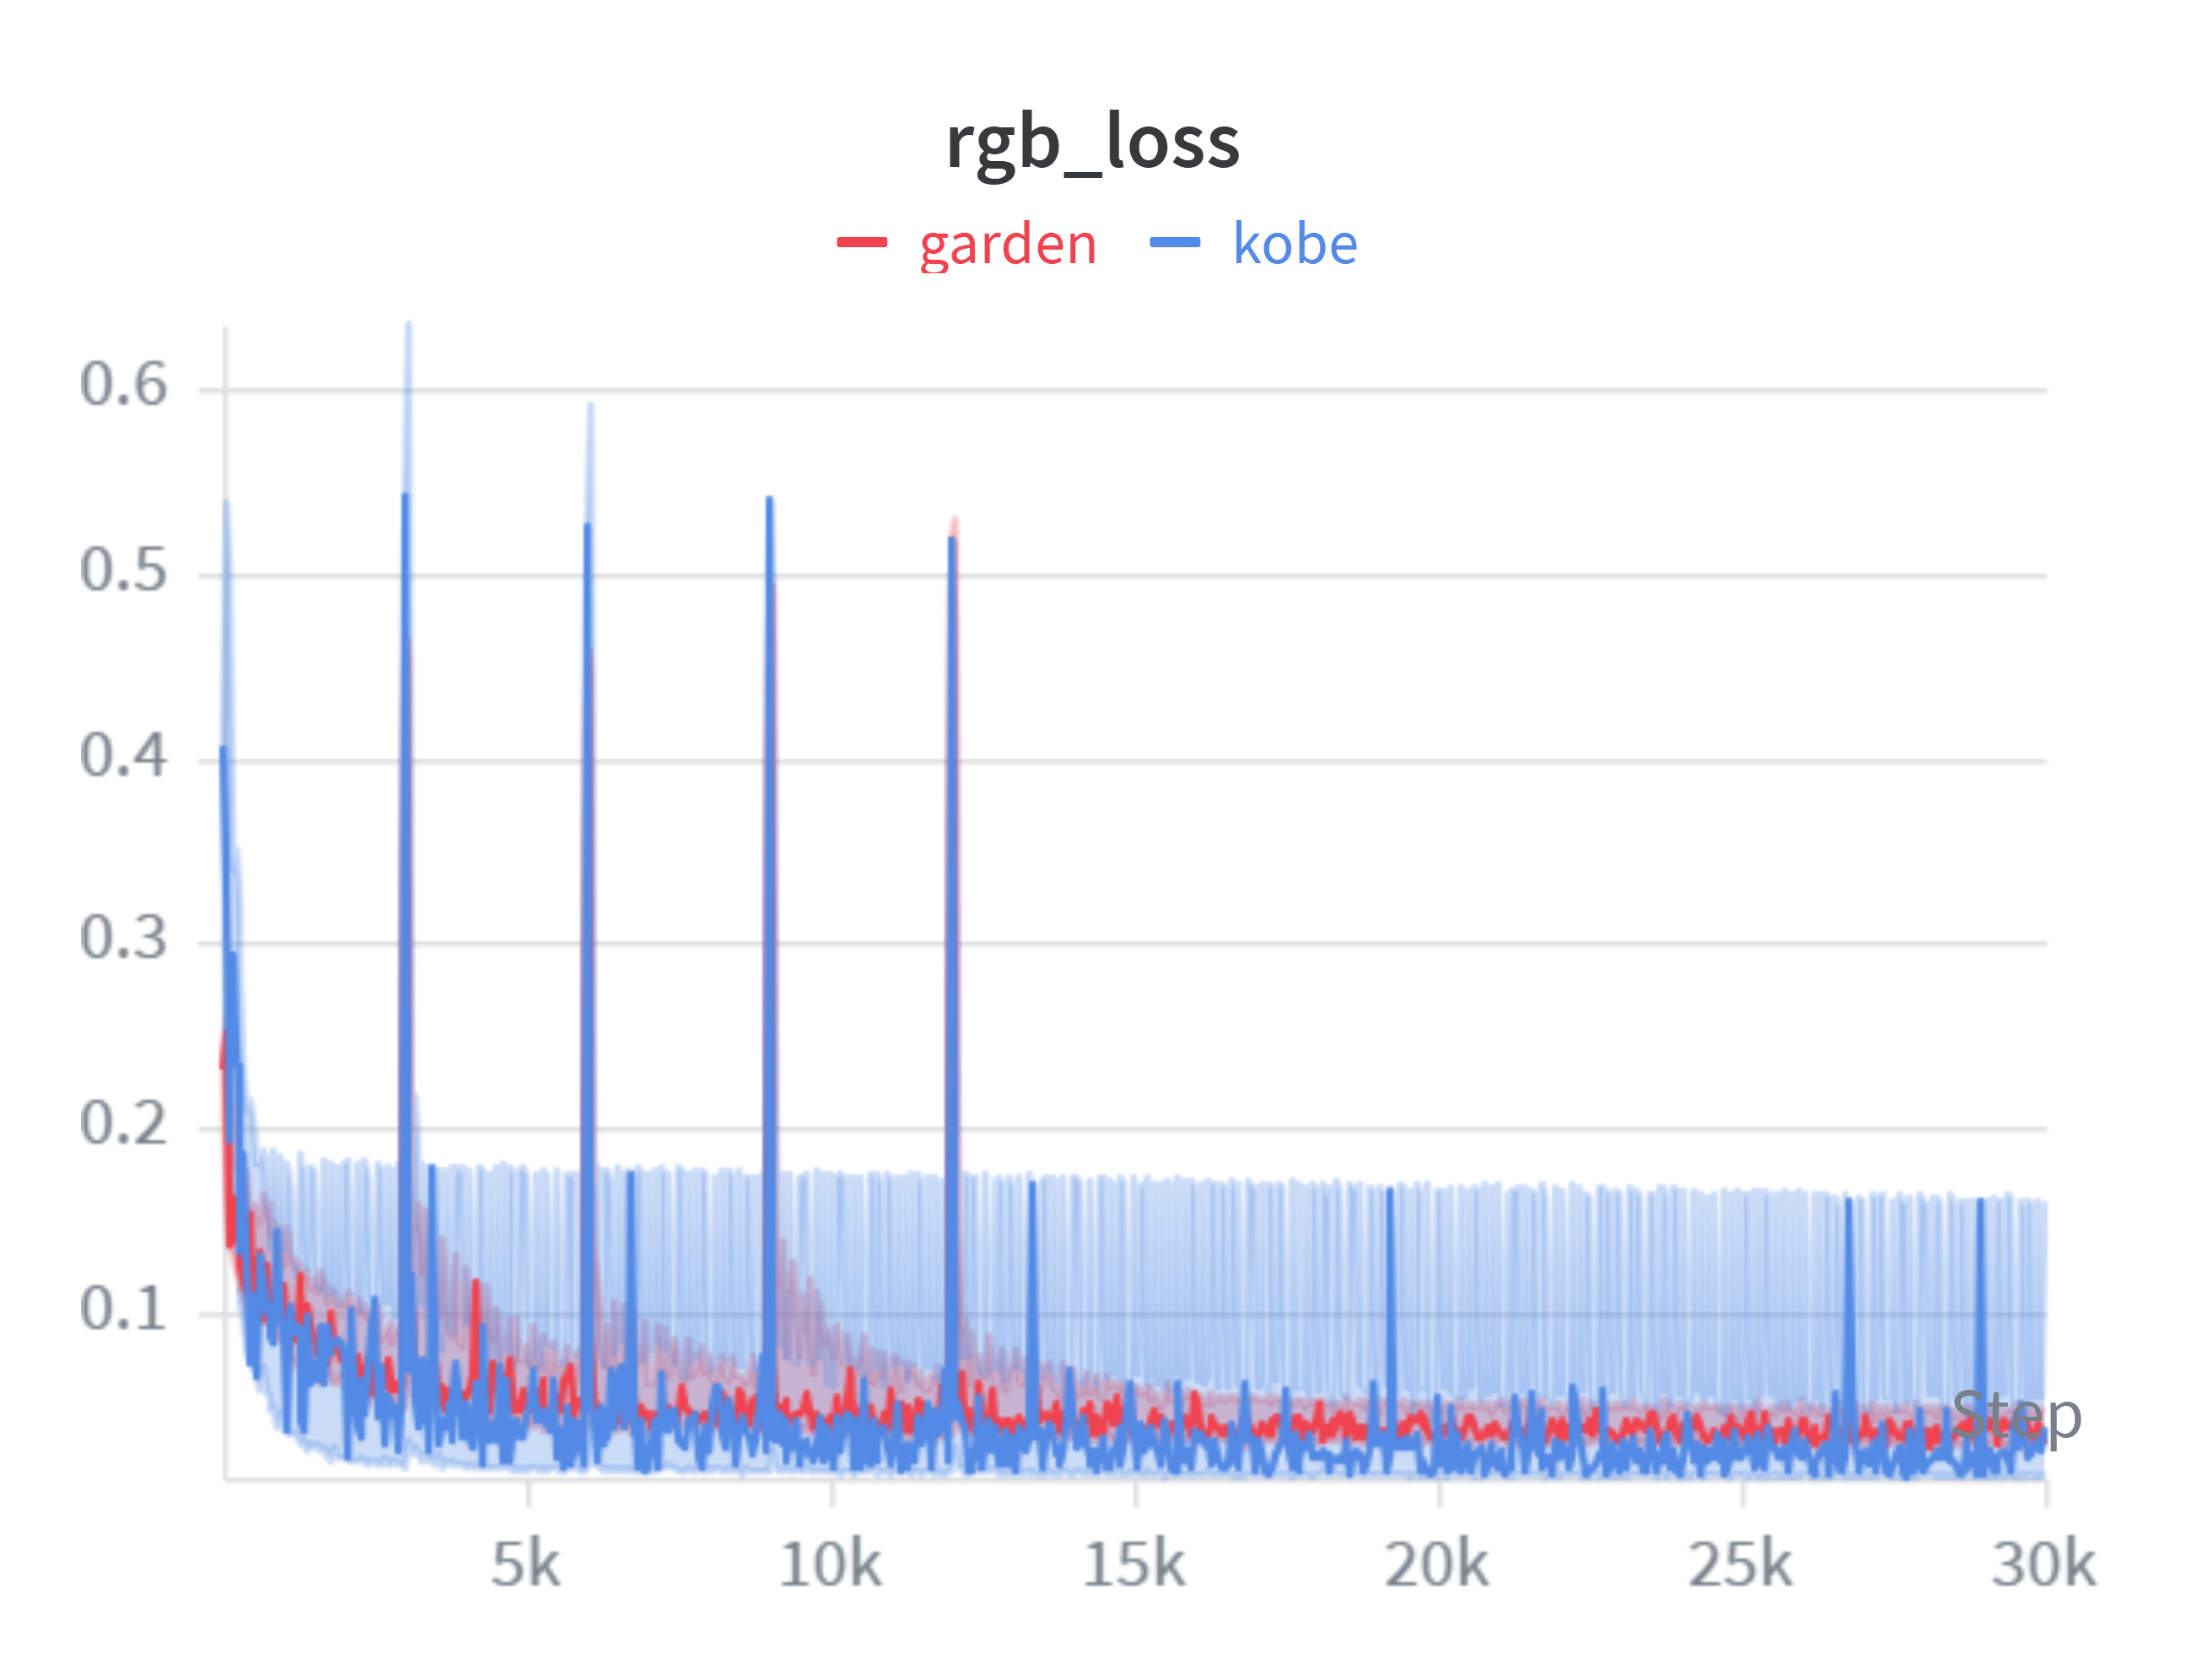
\includegraphics[width=\linewidth]{figures/task1/background/rgb_loss.png}
		\caption{RGB Loss}
	\end{subfigure}
	\hfill
	\begin{subfigure}{0.4\textwidth}
		\centering
		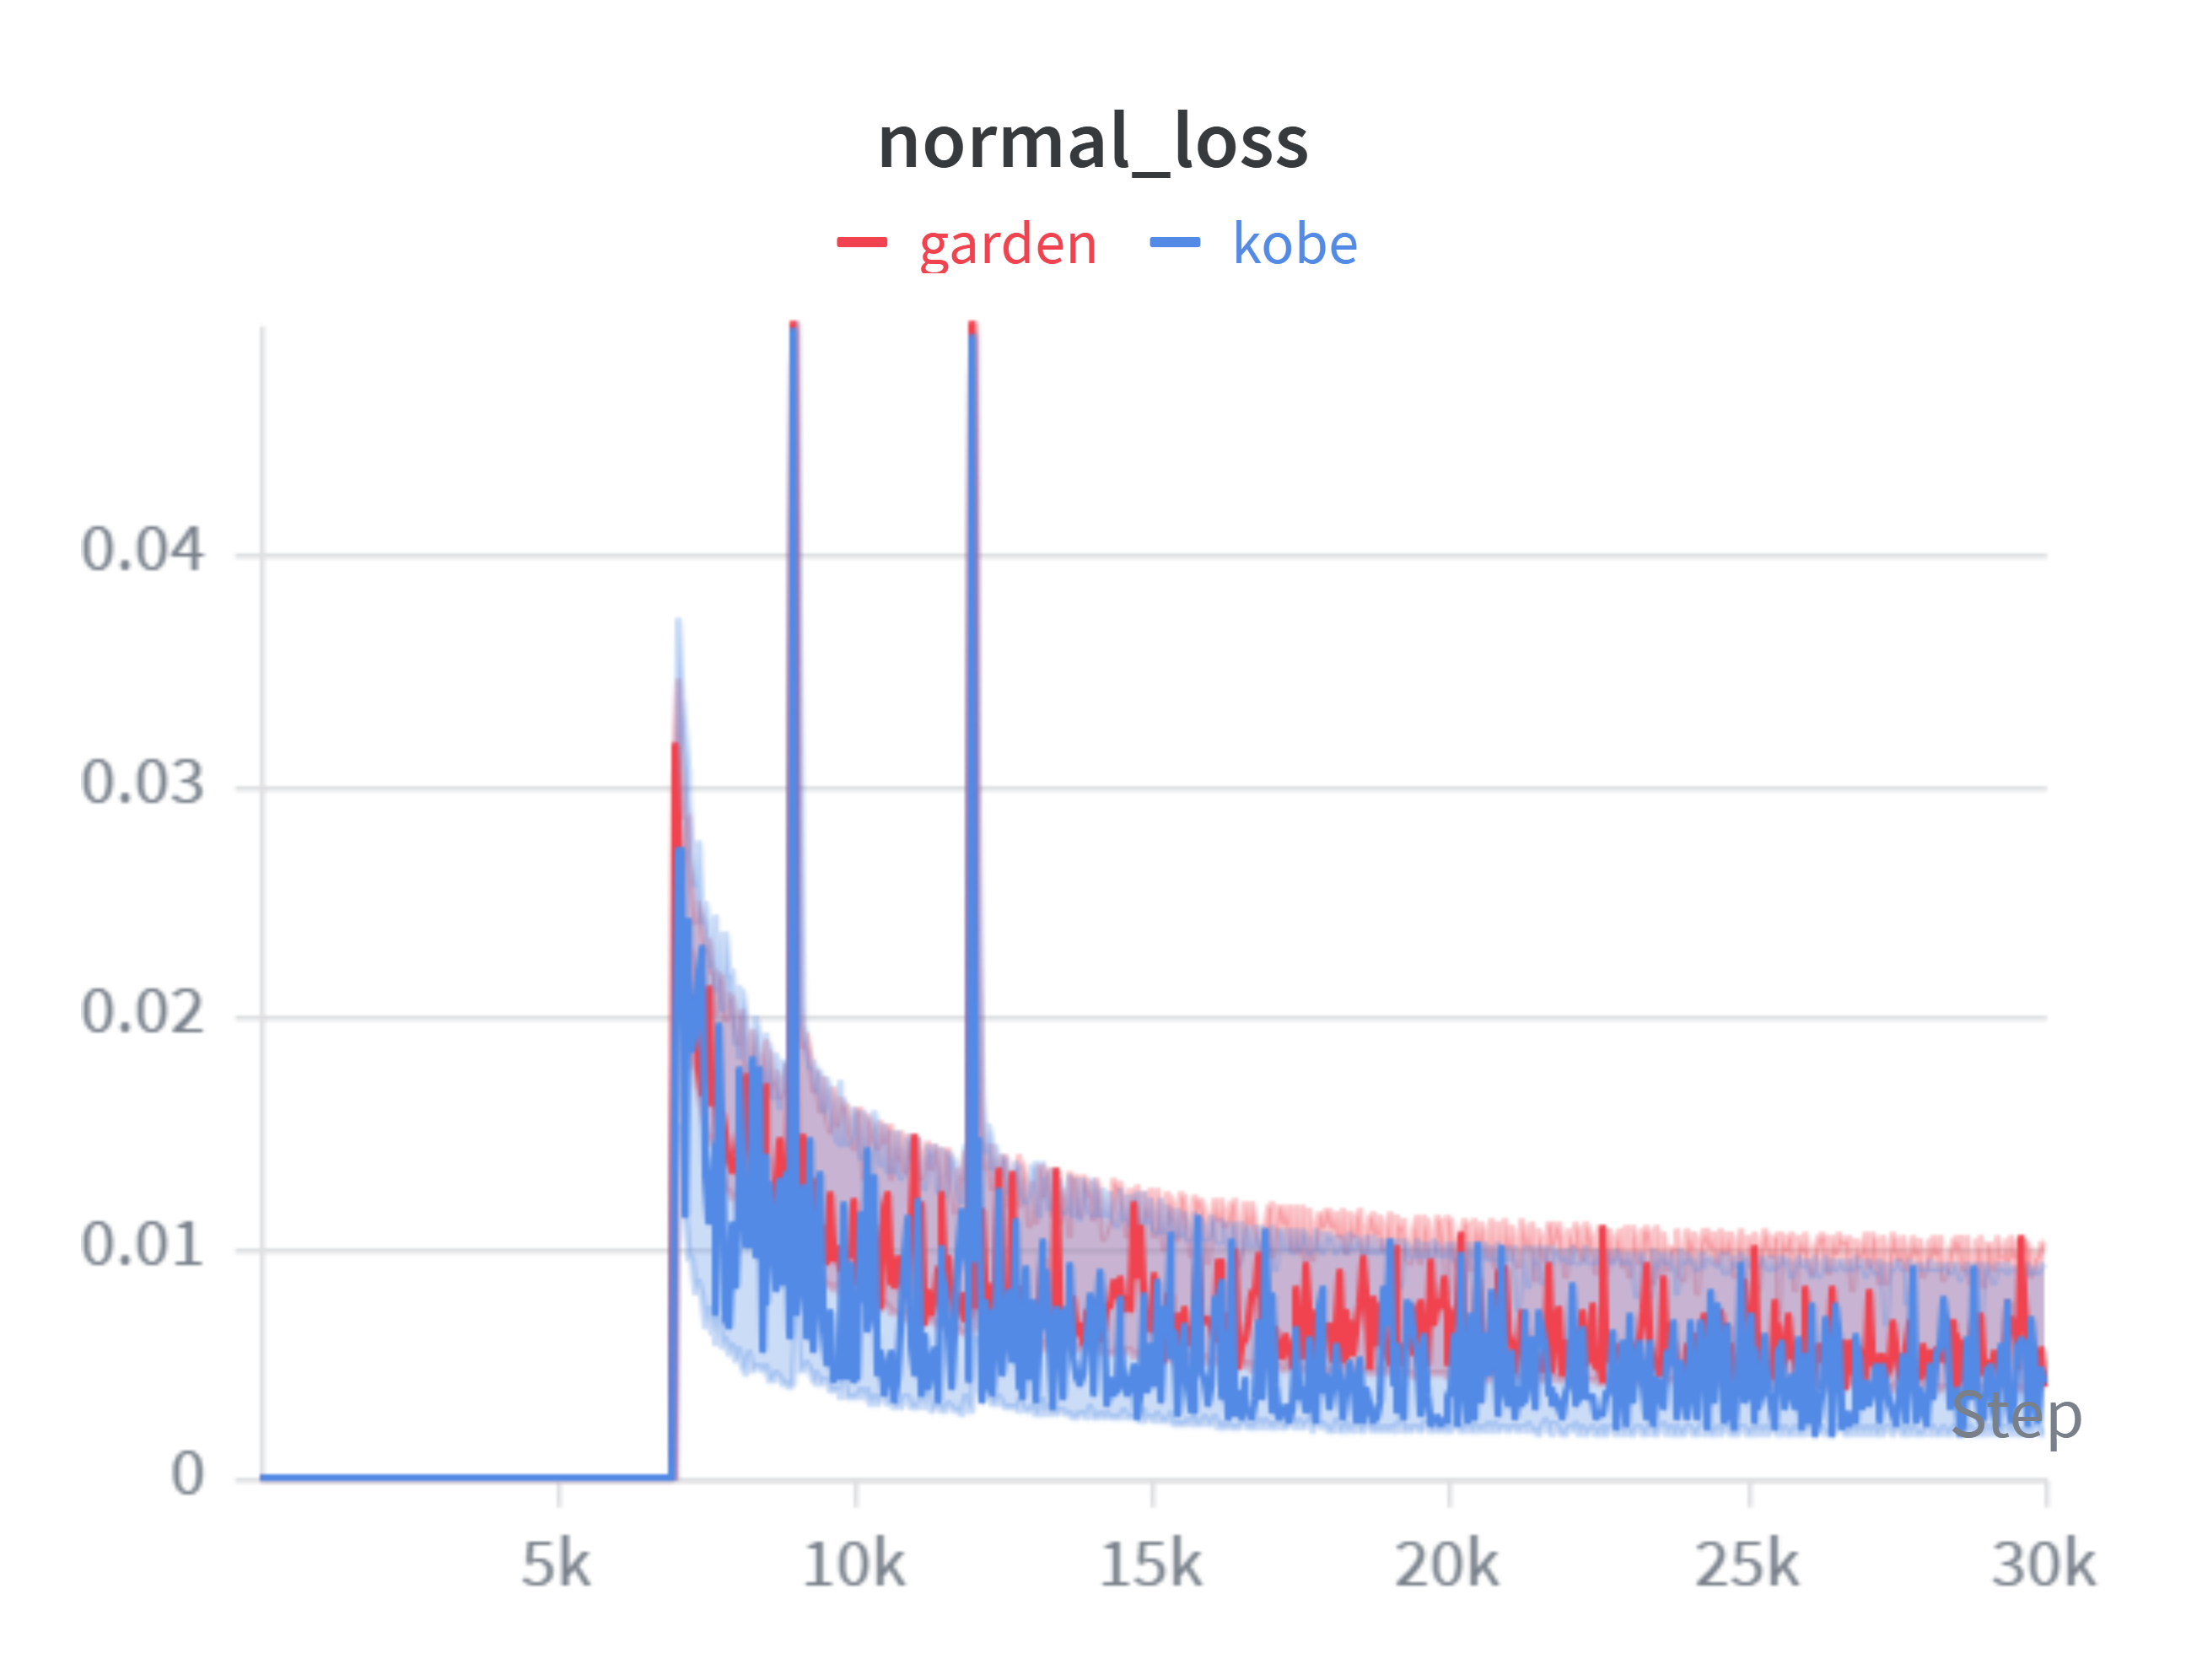
\includegraphics[width=\linewidth]{figures/task1/background/normal_loss.png}
		\caption{Normal Loss}
	\end{subfigure}

	
	\caption{Training Dynamics}
	\label{fig:2DGS Dynamics}

\end{figure}

Both loss curves generally show a downward trend, and the red curve (Garden) is more stable and has fewer peaks than the blue curve (Kobe). This is likely because the Garden has 185 images, twice the dataset of Kobe, thus capturing color and normal information more accurately. Also, Garden captures way more feature points after COLMAP as is shown in Figure~\ref{figure:Feature Points}





\subsection{Quality Accessment}
In this part, all the 3D resources' quality are compared from different perspectives.
\subsubsection{Quantitative indicators}
\begin{table}[H]
	\centering
	\caption{Quantitative Evaluation of Reconstructed Objects and Background}
	\begin{tabular}{c|c|c|c|c}
		\hline
		\textbf{Object} & \textbf{PSNR $\uparrow$} & \textbf{SSIM $\uparrow$} & \textbf{LPIPS $\downarrow$} & \textbf{Training Time(min)} \\
		\hline
		A-Kobe   & 30.94 & 0.9569 & 0.2245 & 55 \\
		\hline
		B-Astronaut & - & - & - & 20 \\
		B-Bunny  & - & - & - &  20\\
		\hline
		C-Firekeeper & 11.669 & 0.1588 & 0.5905 &  60\\
		C-Robot & 8.5543 & 0.5913 & 0.4767 &  60\\
		\hline
		BG-Garden & 30.31 & 0.9080 & 0.1242 & 92 \\
		\hline
	\end{tabular}
	\label{tab:quantitative_results}
\end{table}

In this section, PSNR(Peak Signal-to-Noise Ratio),SSIM(Structural Similarity Inde),LPIPS(Learned Perceptual Ima`ge Patch Similarity) are introduced to access the quality of models. Specifically, Object Bs have no ground truth picture, so we didn't access them this way. \textbf{Also, Object Cs have only 1 picture and the rendering image is manually generated by us, so the accessment is not accurate and can only be taken for reference.}

We can see that Object A and Background Garden have obsessive advantages over Object Cs in geometry accuracy and  mesh details.


For the training time, Object B is the fastest, Object Cs all takes about an hour.
Specifically, Object A(COLMAP+2DGS) is variable.


Considering the training dynamic of Figure~\ref{figure:Feature Points}. We can see that the Garden has 128395 points compared with 5829 points of Kobe at the beginning of the training. This is because of the huge and high resolution dataset of Garden,which helps capture massive amounts of points during the COLMAP part. This takes time(1:12:42hour), but allows faster 2DGS(19:30min). 
\begin{figure}[h]
	\centering
	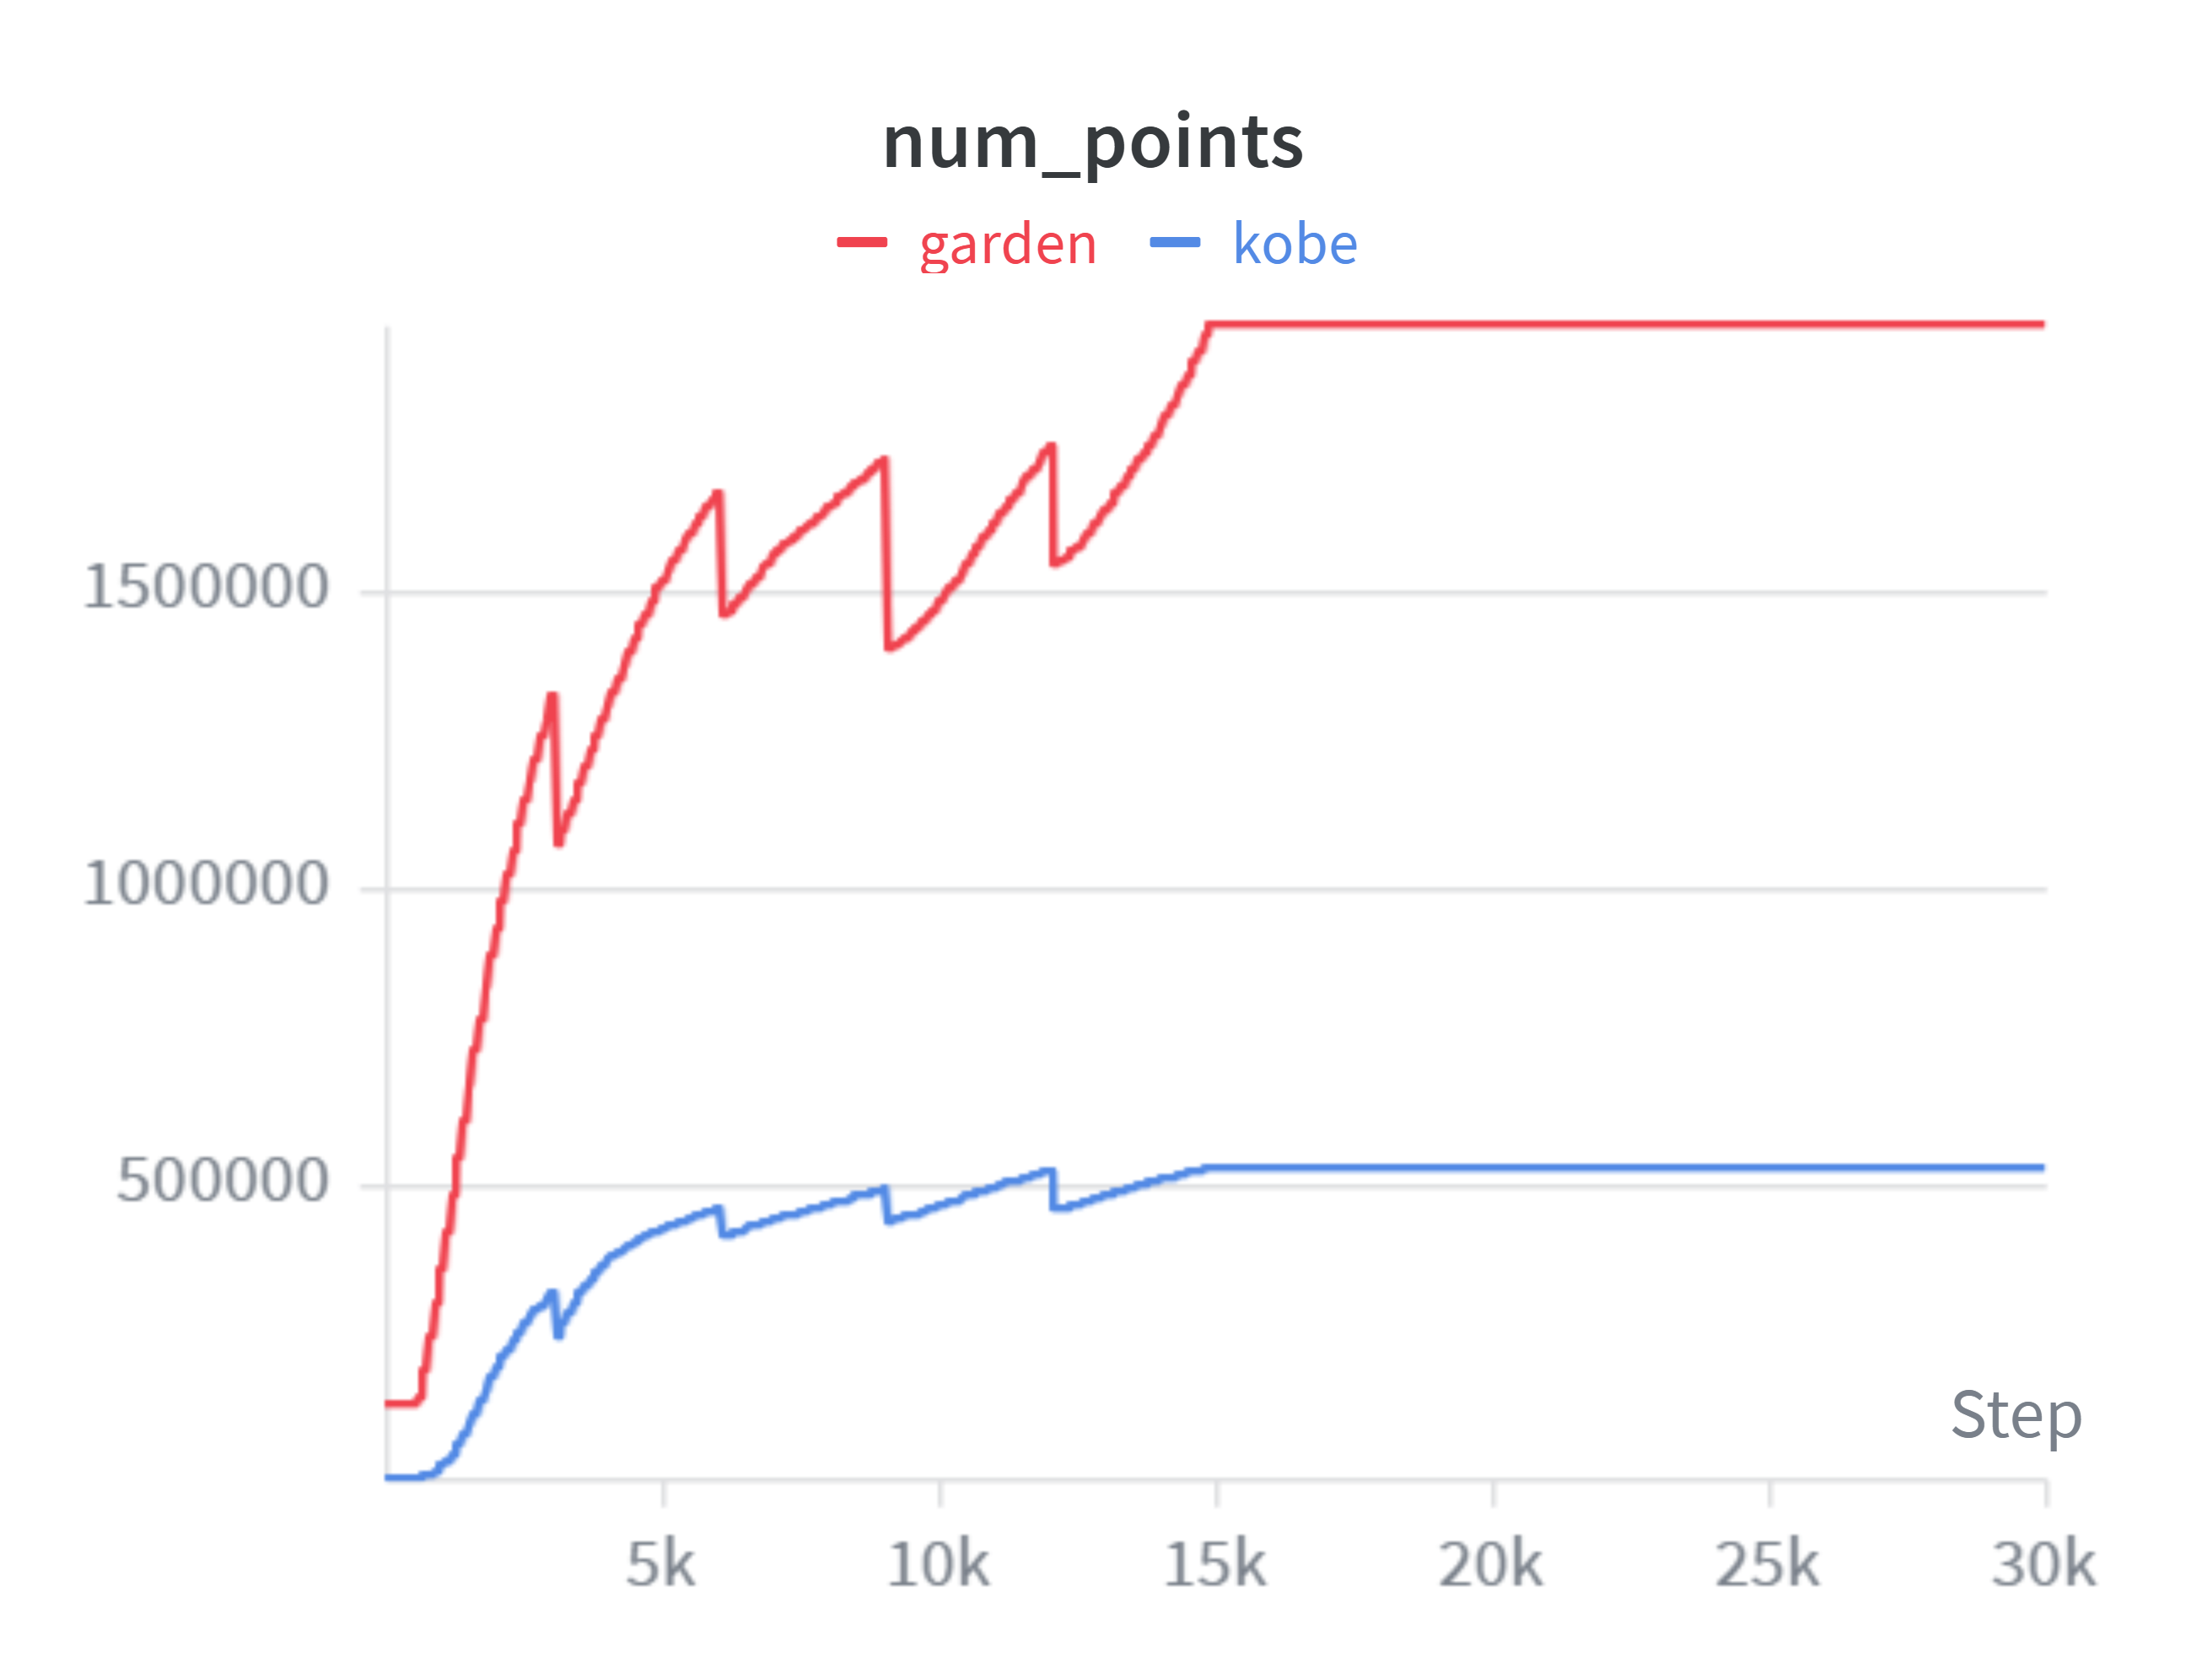
\includegraphics[width=0.4\linewidth]{figures/task1/background/num_points.png}
	\caption{Feature Points}
	\label{figure:Feature Points}
\end{figure}	


\subsubsection{Visual Evaluation}
Considering the different dataset(prompt) of different object, we also try to access the results directly through human eye,which contains some irregular meshes.This can be seen in the videos we offered in the appendix.

For Object A and Background Garden, the visualization looks good and the overall details fit very well except for the places where the pictures don't cover(outside the scene/sky/under the table).

For Object Bs, it's easy to see that the color distribution is not that appropriate as they're in the real world as Figure~\ref{Astronaut Color} Also the details are rough and unsmooth when taking a close look.

For Object Cs, the color distributions are better than Object Bs. The modeling of the front and back are relatively good. However, the side view is worse than the real view, often appearing thinner. This is because the model only receives a frontal photo of the object, making it difficult to accurately judge the thickness:Figure~\ref{fig:firekeeper_vertical} and Figure~\ref{fig:Robot_vertical}. Figure~\ref{fig:objectC_failures} show some of their flaws:
\begin{figure}[h]
	\centering
	
	% 第一组：Firekeeper
	\begin{minipage}{0.45\textwidth}
		\centering
		\textbf{Firekeeper} \\[1ex]
		\begin{subfigure}{0.45\textwidth}
			\centering
			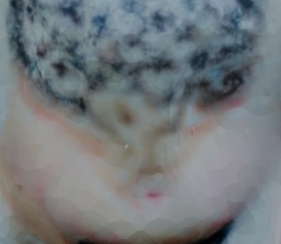
\includegraphics[width=\linewidth]{figures/task1/objectC/firekeeper_wrong_1.png}
			\caption{Mask lacks detail}
		\end{subfigure}
		\hfill
		\begin{subfigure}{0.45\textwidth}
			\centering
			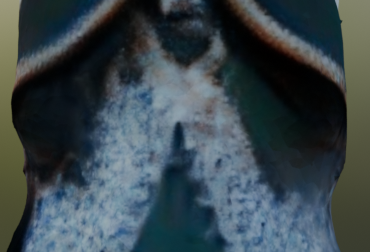
\includegraphics[width=\linewidth]{figures/task1/objectC/firekeeper_wrong_2.png}
			\caption{Hands mistaken as pattern of clothes}
		\end{subfigure}
	\end{minipage}
	\hfill
	% 第二组：Robot
	\begin{minipage}{0.45\textwidth}
		\centering
		\textbf{Robot} \\[1ex]
		\begin{subfigure}{0.45\textwidth}
			\centering
			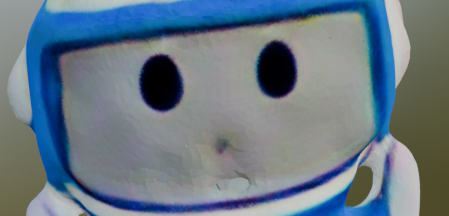
\includegraphics[width=\linewidth]{figures/task1/objectC/robot_wrong_1.png}
			\caption{Poor depth handling}
		\end{subfigure}
		\hfill
		\begin{subfigure}{0.45\textwidth}
			\centering
			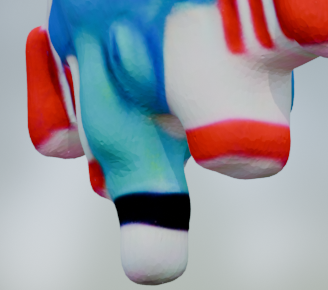
\includegraphics[width=\linewidth]{figures/task1/objectC/robot_wrong_2.png}
			\caption{Joints erased}
		\end{subfigure}
	\end{minipage}
	
	\caption{Failure cases of Object C grouped by subject.}
	\label{fig:objectC_failures}
\end{figure}


\subsection{Fusion Report}

\subsubsection{Fusion Techniques}
Considering that both Object A and Background Scene generate \textbf{point cloud},both Object Bs and Object Cs generate \textbf{mesh}, we export the point cloud as \textbf{gaussian mesh} with the code offered by 2DGS chapter and put all the resources into the Blender.

\subsubsection{Fusion Visualization}
Figure~\ref{fig:Fusion Vis} are some pictures of our fusion results, some include all objects, while some pick one from each category:

\begin{figure}[h]
	\centering
	
	% 第一行：full_1 和 full_2 并排
	\begin{minipage}{0.45\textwidth}
		\centering
		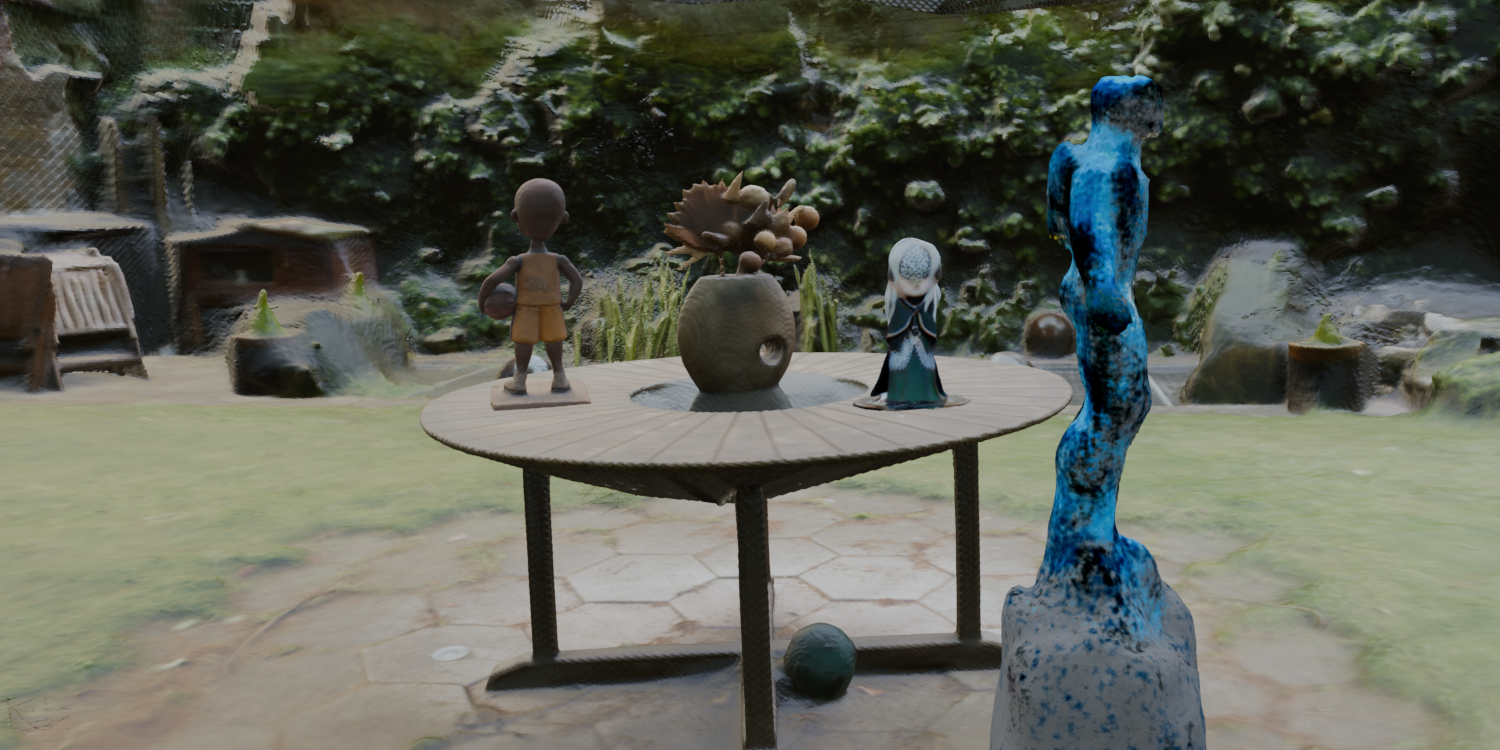
\includegraphics[width=\linewidth]{figures/task1/full_1.png}
	\end{minipage}
	\hfill
	\begin{minipage}{0.45\textwidth}
		\centering
		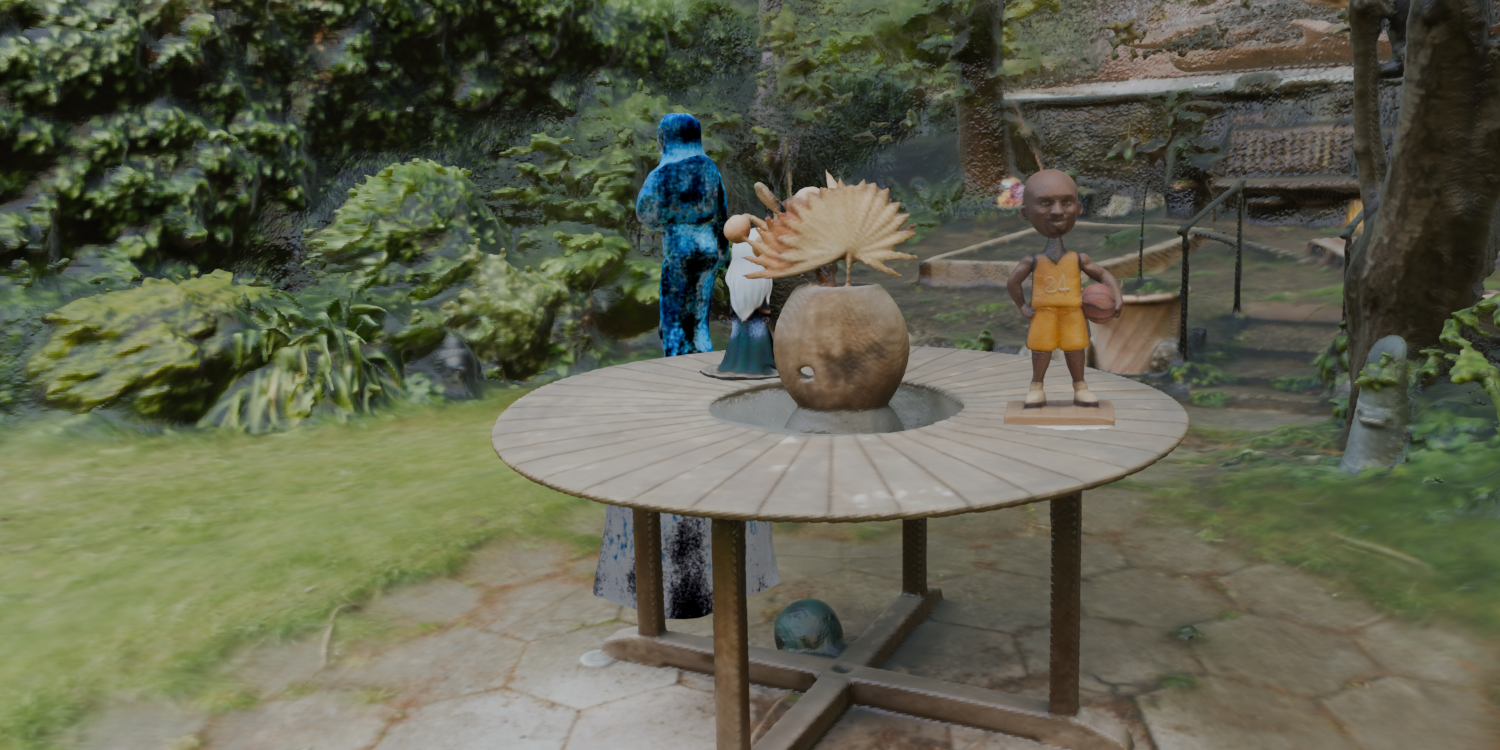
\includegraphics[width=\linewidth]{figures/task1/full_2.png}
	\end{minipage}
	
	\vspace{0.3cm}  % 行间距（可调整）
	
	% 第二行：full_3 和 full_4 并排
	\begin{minipage}{0.45\textwidth}
		\centering
		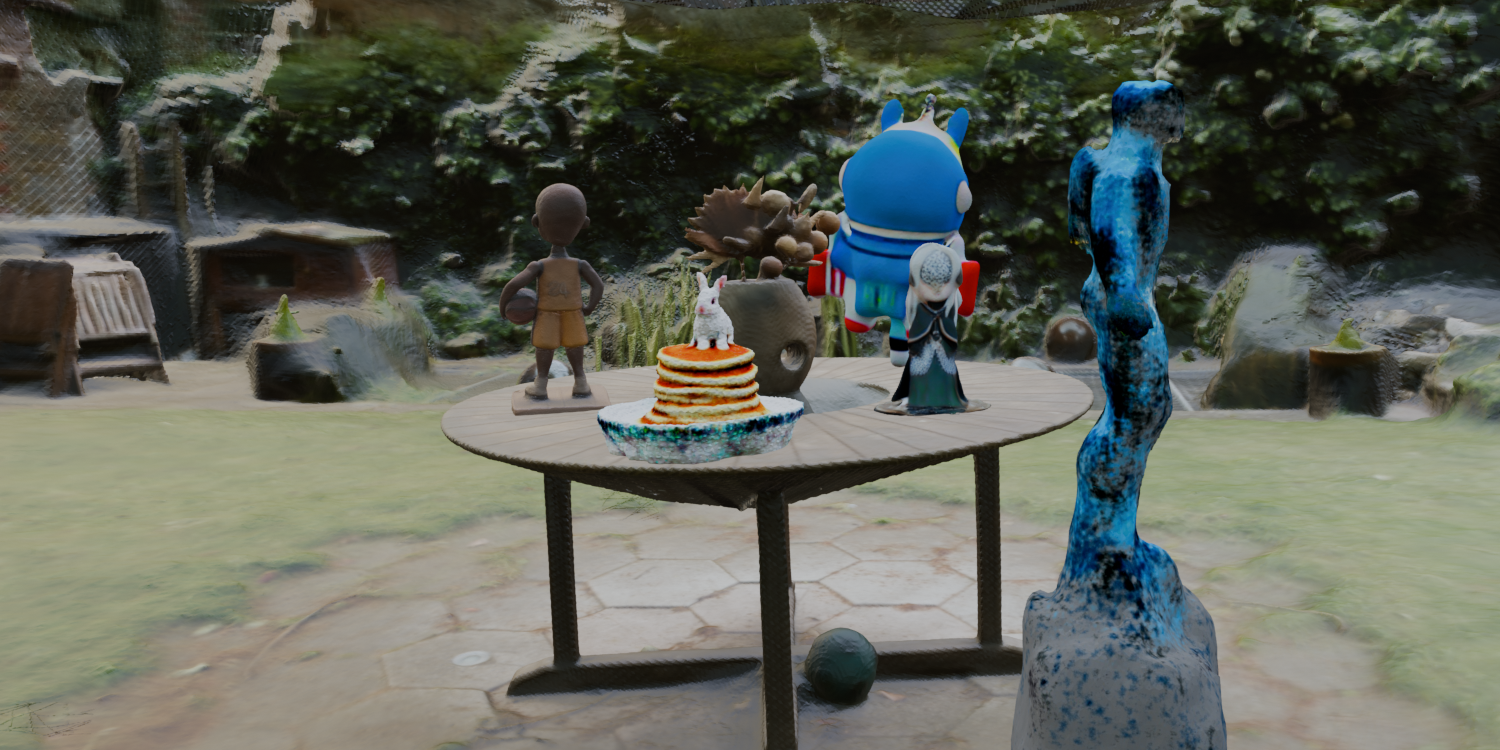
\includegraphics[width=\linewidth]{figures/task1/full_3.png}
	\end{minipage}
	\hfill
	\begin{minipage}{0.45\textwidth}
		\centering
		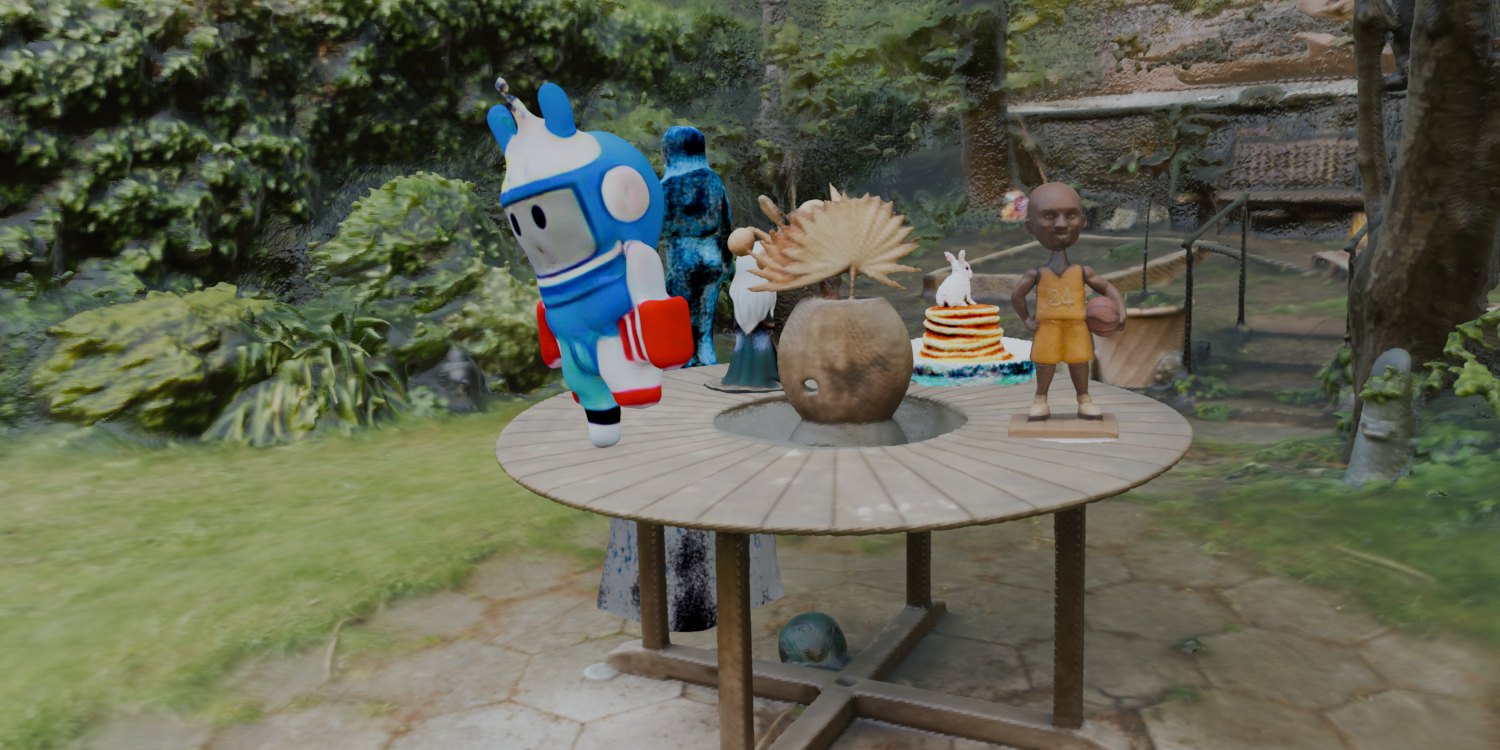
\includegraphics[width=\linewidth]{figures/task1/full_4.png}
	\end{minipage}
	
	\caption{Fusion Visualizations.}
	\label{fig:Fusion Vis}   % 原样保留（包括空格）
\end{figure}

Else, the rendered videos are provided in the appendix (see section~\ref{sec:models}).
\input{sections/task1/Summary.tex}
